%%%%%%%%%%%%%%%%%%%%%%%%%%%%%%%%%%%%%%%%%%
%% TEX main file for the CLAS12 Nim Papers
%%       Do not edit this file
%%%%%%%%%%%%%%%%%%%%%%%%%%%%%%%%%%%%%%%%%%
\documentclass[3p,times,twocolumn]{elsarticle}

\usepackage{lineno, hyperref, multicol, color, xspace, pdfwidgets, enumerate, amssymb, subfig, amsmath, gensymb}


\def \rarr {\rightarrow}
\def \grinp {\includegraphics}
\def \tw {\textwidth}

\modulolinenumbers[5]
\linenumbers

\journal{Nuclear Instruments and Methods A}

\begin{document}

\begin{frontmatter}
\title{The CLAS12 Forward Tagger} 

\author[CEAaddress]{A. Acker}
\author[CEAaddress]{D. Atti\'e}
\author[CEAaddress]{S. Aune}
\author[CEAaddress]{J. Ball}
\author[CEAaddress]{P. Baron}
\author[YORKaddress]{M. Bashkanov}
\author[GEaddress]{M.Battaglieri\corref{mycorrespondingauthor}}
\cortext[mycorrespondingauthor]{Corresponding author}
\ead{marco.battaglieri@ge.infn.it}
\author[DUQaddress]{R. Behary}
\author[DUQaddress]{F. Benmokhtar}
\author[GEaddress]{A. Bersani}
\author[CEAaddress]{Q. Bertrand}
\author[CEAaddress]{D. Besin}
\author[CEAaddress]{T. Bey}
\author[EDINaddress]{P. Black}
\author[JLABaddress]{P. Bonneau}
\author[CEAaddress]{R. Boudouin}
\author[CEAaddress]{M. Boyer}
\author[JLABaddress]{P. Campero Rojas}
\author[GEaddress]{A. Casale}
\author[GEaddress]{A. Celentano}
\author[GEaddress]{R. Cereseto}
\author[RM2address,UNIRTVaddress]{A. Ciarma}
\author[GEaddress]{F. Cipro}
\author[CEAaddress]{G. Charles}
\author[CEAaddress]{G. Christiaens}
\author[CEAaddress]{P. Contrepois}
\author[JLABaddress]{M. Cook}
\author[RM2address,UNIRTVaddress]{A. D'Angelo}
\author[GEaddress]{R. De Vita}
\author[CEAaddress]{M. Defurne}
\author[CEAaddress]{E. Delagnes}
\author[GEaddress]{E. Fanchini}
\author[GWUaddress]{S. Fegan}
\author[EDINaddress]{J. Flemming}
\author[TOaddress]{A. Filippi}
\author[CEAaddress]{M. Gar\c con}
\author[CEAaddress]{F. Georges}
\author[JMUaddress]{K.L. Giovanetti}
\author[GUaddress]{D.I. Glazier}
\author[CEAaddress]{R. Granelli}
\author[CEAaddress]{N. Grouas}
\author[OHIOaddress]{K. Hicks}
\author[JLABaddress]{A. Hoebel}
\author[EDINaddress]{S. Hughes}
\author[CEAaddress]{C. Lahonde}
\author[RM2address,UNIRTVaddress]{L. Lanza}
\author[JLABaddress]{M. Leffel}
\author[CEAaddress]{T. Lerch}
\author[GUaddress]{K. Livingston}
\author[CEAaddress]{I. Mandjavidze}
\author[JMUaddress]{H. S. Mann}
\author[GUaddress]{B. McKinnon}
\author[CEAaddress]{O. Meunier}
\author[JLABaddress]{R. Miller}
\author[GEaddress]{G. Min\'i}
\author[CEAaddress]{Y. Mouden}
\author[GEaddress]{P. Musico}
\author[GEaddress]{M. Osipenko}
\author[GEaddress]{G. Ottonello}
\author[GEaddress]{F. Parodi}
\author[JLABaddress]{E. Pasyuk}
\author[GEaddress]{P. Pollovio}
\author[GEaddress]{F. Pratolongo}
\author[CEAaddress]{S. Procureur}
\author[GEaddress]{R. Puppo}
\author[GEaddress]{C. Rossi}
\author[CEAaddress]{M. Riallot}
\author[GEaddress]{M. Ripani}
\author[RM2address,UNIRTVaddress]{A. Rizzo}
\author[CEAaddress]{F. Sabati\'e}
\author[NSUaddress]{C. Salgado}
\author[EDINaddress]{G. Smith}
\author[GUaddress]{D. Sokhan}
\author[EDINaddress]{I. Stankovic}
\author[GEaddress,UNIGEaddress]{M. Taiuti}
\author[GEaddress]{A. Trovato}
\author[CEAaddress]{M. Vandenbroucke}
\author[CEAaddress]{E. Virique}
\author[YORKaddress]{D. Watts}
\author[JLABaddress]{C. Wiggins}
\author[YORKaddress]{N. Zachariou}
\author[JLABaddress]{L. Zana}

\address[CEAaddress]{IRFU, CEA, Universit\'e Paris-Saclay, F-91191 Gif-sur-Yvette, France}
\address[YORKaddress]{University of York, York YO10 5DD, United Kingdom}
\address[GEaddress]{INFN - Sezione di Genova, Via Dodecaneso 33, I-16146 Genova,Italy}
\address[DUQaddress]{Duquesne University, Pittsburgh, PA 15282, USA}
\address[RM2address]{INFN, Sezione di Roma Tor Vergata, 00133 Rome, Italy}
\address[UNIRTVaddress]{Universit\'a di Roma Tor Vergata, 00133 Rome Italy} 
\address[GWUaddress]{The George Washington University, Washington, DC 20052, USA}
\address[EDINaddress]{University of Edinburgh, Edinburgh EH9 3FD, United Kingdom}
\address[TOaddress]{INFN, Sezione di Torino, 10125 Torino, Italy}
\address[JMUaddress]{James Madison University, Harrisonburg, VA 22807, USA}
\address[GUaddress]{University of Glasgow, Glasgow G12 8QQ, United Kingdom}
\address[OHIOaddress]{Ohio University, Athens, OH 45701, USA}
\address[NSUaddress]{Norfolk State University, Norfolk, VA 23504, USA}
\address[UNIGEaddress]{Universit\'a degli Studi di Genova, Via Dodecaneso 33, I-16146 Genova,Italy} 
\address[JLABaddress]{Thomas Jefferson National Accelerator Facility, Newport News, VA 23606, USA}

\begin{abstract}The High Threshold Cerenkov Counter (HTCC) is one of the detector systems of the CLAS12 spectrometer, and is used to generate fast trigger signal in electron experiments. The HTCC is installed in front of the R1 Drift Chambers and introduces a minimal amount of additional material within working acceptance. The HTCC is one unit whose core component is a multifocal mirror that consists of 60 lightweight composite ellipsoidal mirrors. It is important that the HTCC provides efficient coverage of the CLAS12 acceptance with no gaps or overlaps. In order to achieve this, each sector of the CLAS12 spectrometer is covered by 2 identical half-sector mirrors that focuses Cerenkov light on eight phototubes. The HTCC has a total of 48 channels with Electron Tubes 9823QKB PMTs that have a 5" quartz face plate to detect Cerenkov light. The system provides a high rejection of charged $\pi$-mesons and low background noise for reliable identification of scattered electrons. The details of the design, construction, calibration, and performance results of the HTCC are presented in the following paper. 

\end{abstract}

\end{frontmatter}

\date{\today}

\section{Overview}

torus overview description \cite{einstein}



\section{Requirements}

torus requirements description


\section{Design(Chris, Sergey)}

CLAS12 Data Aquisition system is designed as pipeline-style network-based system. Data taking process starts from front-end components. Those components can have different hardware and software implementation but have to follow certain requirements to be compatible with the rest of the system. Currently front-end components used are commercial VME/VXS crates, commercial Linux servers and JLAB-designed VXS Trigger processor boards. VTPs installed in VXS crates but read out by DAQ as independent components. All components are running on 250MHz clock discributed over OM3 rated parallel optic fibers. The same fiber system is used to distribute sync reset and trigger signals and to collect busy signals from all front-end electronics.

All front-end components are connected to Event Builder (EB) which is multi-threaded program running on multi-core Linux server. Most connections are 1Gbit ethernet links. For several components generating significant data rate 10Gbit ethernet connection is used.

Complete events are sent to Event Transfer (ET) System. ET is multi-threaded program providing data ring where various data processing programs can be attached to monitor data quality online. It can be run on the same server as EB, or can be used to create sequensial chain of servers to increase data processing power.

Last component in the data chain is Event Recorder (ER). It is multi-threaded program receiving data from ET system and recording it to the disk. Multi-stream mode is available, allowing to write several files in parallel to the same or different disk partitions to increase writing performance. Event order in multi-stream mode is preserved.

CLAS12 DAQ System diagram is shown on Fig.~\ref{fig:DAQdiagram}.

\begin{figure}[hbt]
	\centering
	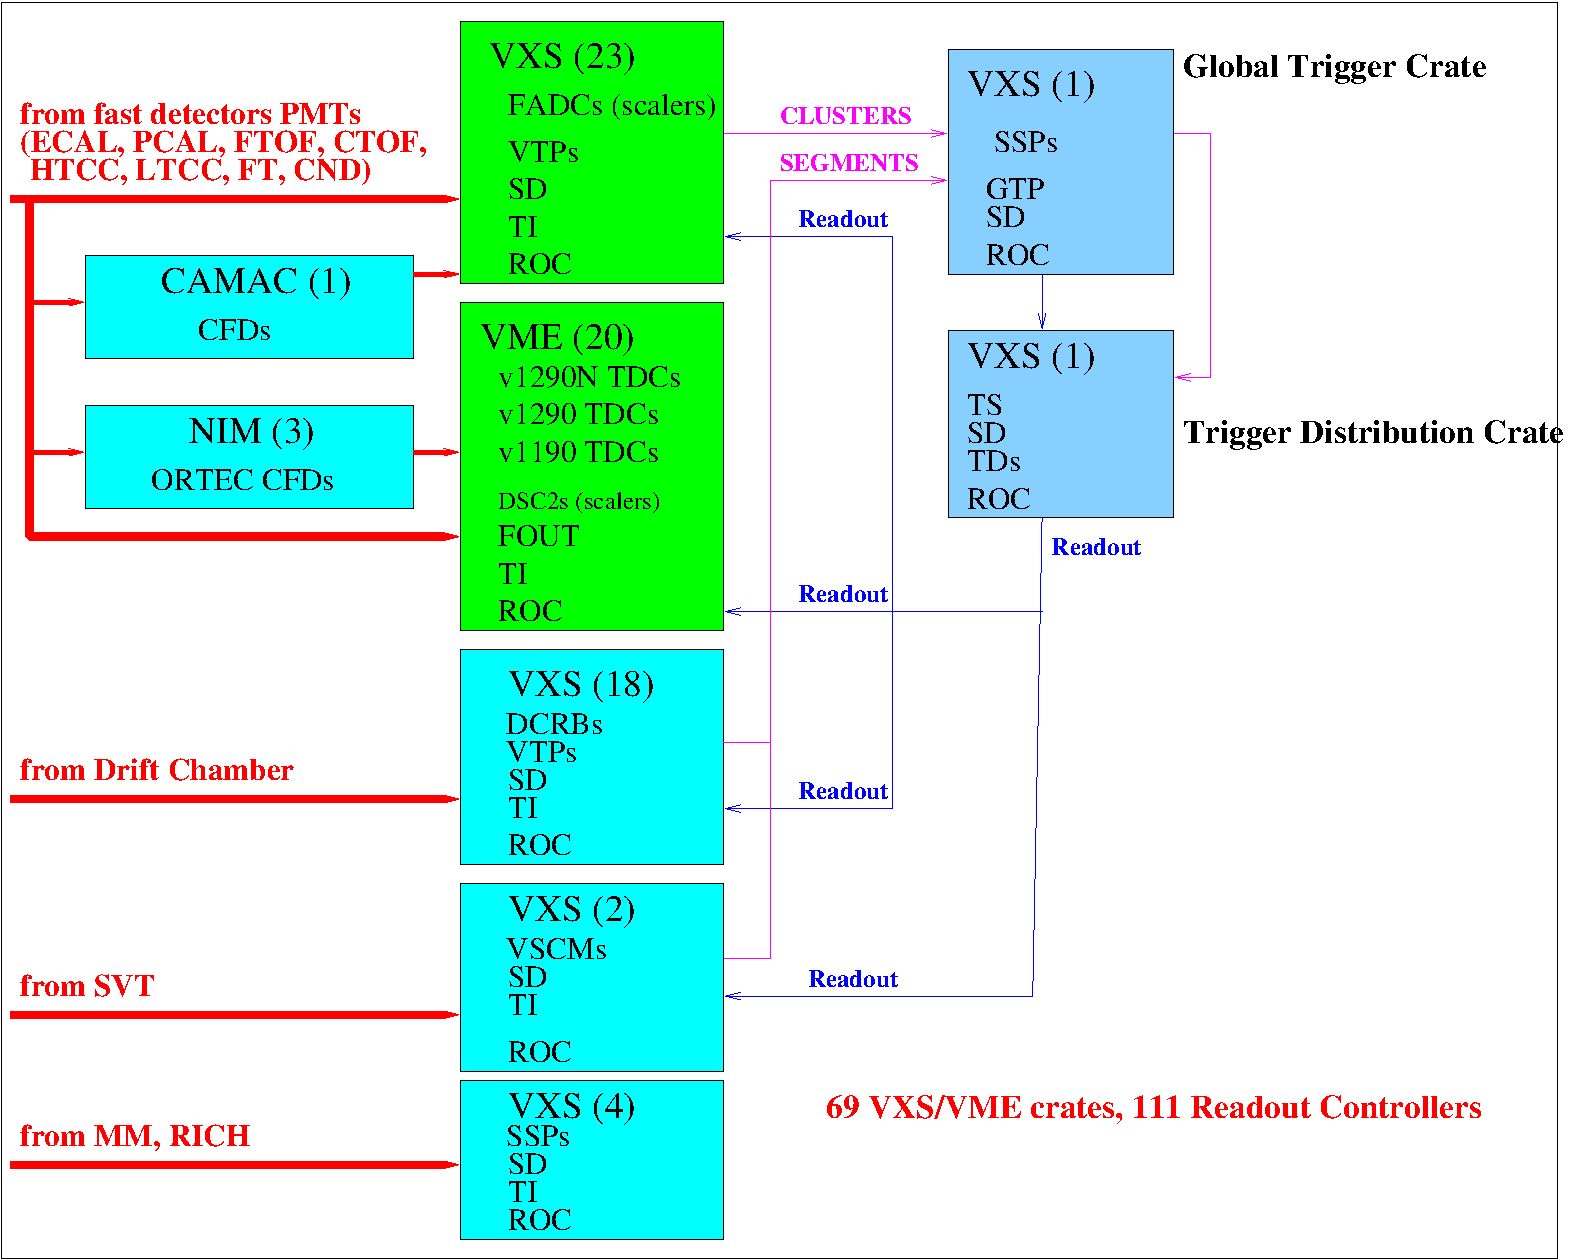
\includegraphics[width=1.0\columnwidth,keepaspectratio]{img/CLAS12_HARDWARE_2.pdf}
	\caption{CLAS12 Data Aquisition System Diagram}
	\label{fig:DAQdiagram}
\end{figure}


\section{Hardware Components}

New instrumentation modules have been designed by JLab that take advantage of the higher performance and elegant back-plane connectivity of the VITA 41 standard or ``VXS'', defined as VME with serial extensions. 
VXS was selected as the 12~GeV data acquisition back-plane foundation for the front-end detector readout and trigger hardware interface because this standard offered a method to easily synchronize and pass signals between each of the payload slots to a central switch fabric slot. At JLab a dual star back-plane configuration is used, and one switch slot is used for the trigger processing and one switch slot is used to distribute the essential timing and synchronization signals to each of the front-end boards.

The trigger processor switch slot board manages the high-speed gigabit signaling from each of the payload slots, where eight differential pairs connect from the payload slots to the switch slots. The VXS crates are manufactured by WIENER and the back-plane can support up to 8~Gb/s. The payload boards use Xilinx Virtex V technology, and these FPGAs have up to 6.25~Gbps transceivers. The payload boards are designed to run these high-speed gigabit transceivers at a maximum of 5~Gpbs to transfer trigger data to the trigger processor module. 

The design challenges for reliable and successful transmission of gigabit serial data over the VXS backplane requires the investment of high-speed circuit board layout and routing tools.  The FPGA selection requirements include at least four full duplex gigabit transceivers, user I/O pin count $>$~500, and fast integrated block memory with multi-rate FIFO logic. We use circuit board routing simulation tools such as Mentor Graphics HyperLynx [\ref], which are invaluable for critical simulation and verification of circuit board signal integrity for the gigabit transmission paths before the manufacturing process.  The FPGA devices that we use are capable of 6.25~Gb/s serial transfer, and we have designed our circuit boards with signal integrity techniques using standard FR4 circuit board material to achieve $>$~2.5~Gb/s, which meets the data transfer bandwidth requirements. 
Another significant investment required for the hardware verification of the gigabit transceivers was a digital signal analyzer with 8~GHz bandwidth to measure and record the backplane and fiber optic gigabit transceiver performance and to perform jitter analysis on the critical system clock and synchronization signals with at least 1~ps resolution.  We used the Tektronix jitter analysis software which is a critical tool for the verification of our system clock, and for measurements of the phase controlled jitter attenuated clock provided by the Signal Distribution (SD) switch card in every crate. The investment of firmware development tools from FPGA industry leaders Xilinx and Altera were also taken into consideration for the upgrade path to VXS. We use the Xilinx Aurora protocol for serial transmission as it is robust and simple, and is included with the FPGA development tools.  


\subsection{Fiber Optic Trigger distribution system}

As shown in Fig.~\ref{fig:hardwarediagram}, the digital sum value from each VTP in the front-end crate, and the distribution of the global clock, synchronization, and trigger commands from the global trigger hardware, use a separate fiber optic cable.  The crate sum fiber link is shown in orange, and the critical timing signals distributed to each front-end crate are blue.  Each fiber optic link makes use of the Avago POP4 fiber optic transceivers and parallel OM3-rated glass fiber cable with MTP connections. These fiber optic transceivers operate at 3.125~Gb/s for an aggregate bandwidth of 10 Gb/s which is ample enough for the summing information that is sent forward to the global trigger processing hardware.  The fiber link used for the distribution of the global clock, critical timing signals, and trigger commands runs at 1.25~Gb/s.

\begin{figure}[hbt]
	\centering
	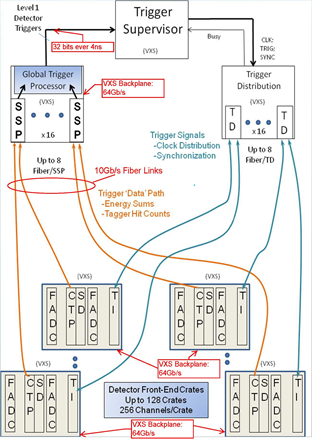
\includegraphics[width=1.0\columnwidth,keepaspectratio]{img/hardware_diagram.png}
	\caption{Hardware diagram with the implemented fiber links scheme.}
	\label{fig:hardwarediagram}
\end{figure}


\subsection{VXS/VME crates}

Previous experiments with the original CLAS spectrometer (see \cite{clas-nim}) used the VXI standard, which was a new extension of the original VME standard. VXI offered a method to distribute clock and other timing signals with low skews via the back-plane. 9U circuit boards were used that offered a large number of front panel input/output connections to handle the six sectors of the CLAS detectors that contributed to the level 1 trigger. The detector signals were acquired with FastBus ADC and TDC or in some instances, from VME or even CAMAC modules. 

During the initial design phase of the 12~GeV experiments the requirements of a 200~KHz sustained trigger rate demanded that the front-end modules adopt a new method of handling precision timing and synchronization over dozens of front-end crates. The latest technology at the 12~GeV inception included FPGA devices with high-speed serial transceivers built into the silicon fabric. A new VME extension was also emerging at the same time, which was labeled VXS, and defined a new high-speed gigabit connector with links between the VME slots and eight serial links to common switch slots. The VXS standard was declared as VITA 41 and several new standards have emerged in the past decade that expand the use of gigabit serial transmission via the crate back-plane. For the 12~GeV experiment era, we now have thousands of custom VXS payload and switch slot modules and hundreds of VXS front-end crates. Complex experiments and high channel count detectors make use of these custom VXS boards  designs for all four experimental halls at JLab.

\subsection{VME Crate Controllers}

The high-speed data physics acquistion and trigger systems for the JLab 12~GeV experiments have been standardized on the VME64X and VXS backplane and crate enclosure form-factor. In addition to the custom electronics that reside in these crates, there must also be a single ``controller'' for each crate. Considering all four experimental halls, this exceeds 100 controllers.

There are many commercial off-the-shelf options for this type of controller, and our general requirements do not extend beyond what is currently commercially available. We do have some specific requirements that narrowed the viable choices.

We purchased VME controllers from several vendors for development purposes and made a significant investment in custom software that runs on all of the existing boards. We also benchmarked our code and have come to expect certain ``minimum'' requirements for performance from the chosen architecture within an specified Linux operating system.

We also expect a certain minimum 10 year timeframe in which these controllers will be supported by the vendor with respect to the avilable parts, repair, and software updates. VME controller requirements are summerized in following list:

\begin{itemize}
	\item Single slot VME form-factor - no required rear transition module
	\item Intel Core i7 dual or quad core embedded processer 2~GHz (or greater)
	\item Hyperthreading and 64~bit arch support
	\item 4 GBytes DDR3 (1066~MHz) ECC SDRAM (or greater)
	\item Front panel gigabit ethernet and serial port console
	\item 1 x4 PCI Express XMC expansion slot (or greater)
	\item VME320-interface using the Tundra Tsi148 chip
	\item support for all VME transfer modes including 2eSST
	\item VXS optional: interface supporting both VITA 41.3 (Gig E) and 41.4 (PCIe) standards.
\end{itemize}

After several different boards were evaluated we purchased XVR16 Intel forth Generation 4-core i7-based rugged VME single board computers from GE (see Fig.~\ref{fig:XVR16diagram}). They were installed in the 70+ crates for CLAS12 and have demonstrated excellent performance and reliability. Most of the controllers send data over their built-in 1~GBit link, while for few of them, a 10~GBit daughter board was installed to increase the bandwidth. The maximum data rate from a single crate in CLAS12 never exceeds 130~MB/s, and with that rate 4-core controllers are able to handle the VME data polling, data processing, and sending data over the network without any issues. 

\begin{figure}[hbt]
	\centering
	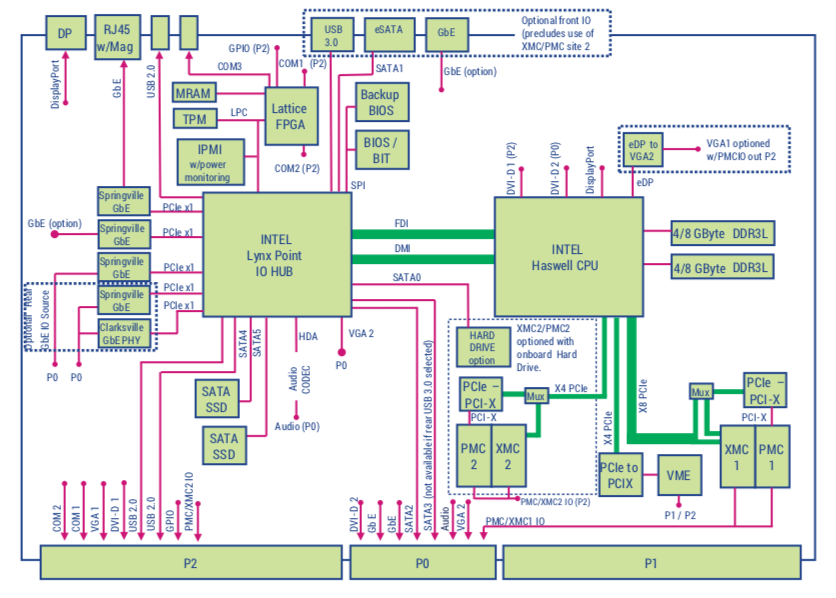
\includegraphics[width=1.0\columnwidth,keepaspectratio]{img/XVR16_diagram.png}
	\caption{Block diagram of the XVR16 VME crate controller}
	\label{fig:XVR16diagram}
\end{figure}



\subsection{Trigger Distribution System Modules (TS, TD, TI)}
	
The TCS (TRIGGER, CLOCK, SYNC, and BUSY) distribution system \cite{tcs-ref} is the hardware interface to bridge the trigger and the DAQ.  The TCS system receives the trigger decision from the trigger system, and initiates data readout for the DAQ system by distributing the readout trigger (TRIGGER) signal.  Additionally, it distributes a 250~MHz system clock (CLOCK) to pipeline the system, and it distributes an encoded synchronous signal (SYNC) for the system synchronization.  It monitors the frontend electronics’ status (BUSY) and makes sure of the smooth data readout of the experiments. Fig.~\ref{fig:TCSdiagram} shows a diagram of the trigger and TCS distribution.

\begin{figure}[hbt]
	\centering
	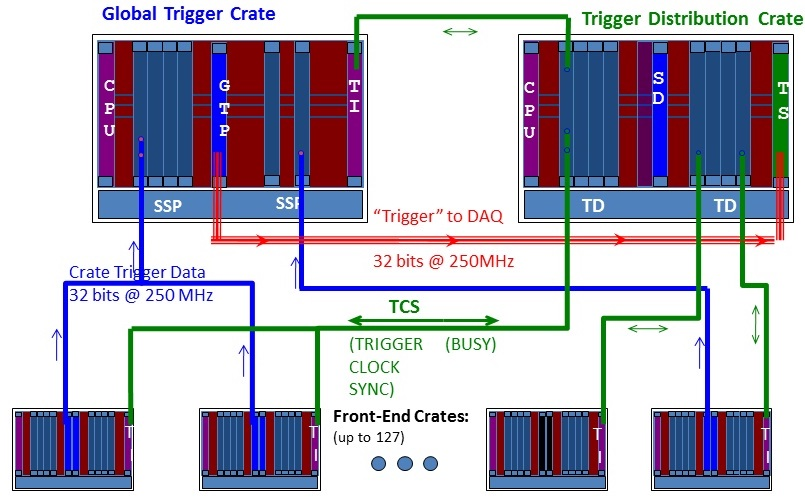
\includegraphics[width=1.0\columnwidth,keepaspectratio]{img/TCSdiagram.jpg}
	\caption{Diagram of the trigger and TCS distribution. The VTP boards generate triggers using detector signals from the front end crates.  The final trigger decisions, up to 32 trigger types, are sent from VTP to TS for data readout.  The TS distributes the TCS to the TD through SD and the backplane, then to the front end crate through optic fiber and TI.  The TI collects the front end boards busy signals and sends to TD, then throttle (disable) the readout trigger distribution on TS.
}
	\label{fig:TCSdiagram}
\end{figure}


The main hardware of the TCS distribution system includes a Trigger Supervisor (TS \cite{ts-ref}) board (see Fig.~\ref{fig:TSused} and ~\ref{fig:TSdiagram}), Signal Distribution (SD \cite{sd-ref}) boards, Trigger Distribution (TD \cite{td-ref}) boards  (see Fig.~\ref{fig:TDused}), Trigger Interface (TI \cite{ti-ref}) boards  (see Fig.~\ref{fig:TIused} and ~\ref{fig:TIdiagram}), VXS crates, and optic fibers.  The TS board, one SD board, and up to sixteen TD boards are located in the global TCS distribution VXS crate.  One TI board and one SD board and/or one FANIO board are located in each front-end crate.  The electronics boards were custom designed and produced for the 12 GeV upgrade.  Field Programmable Gate Arrays (FPGA) are used for TCS generation, control, and decoding.  Optical fibers and high-speed differential backplane connections are used to transmit signals at high speed over long distances.  

\begin{figure}[hbt]
	\centering
	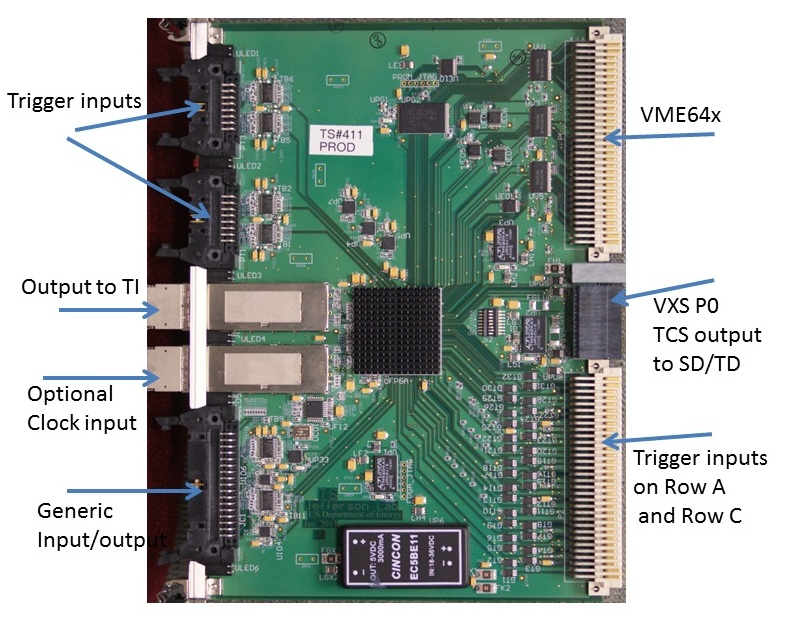
\includegraphics[width=1.0\columnwidth,keepaspectratio]{img/TSused.jpg}
	\caption{Trigger Supervisor (TS) board.  The TS board is a 6U by 160mm VME board with VXS connector.  It generates and distributes the readout triggers, synchronization signals, and clock (either from the front panel input or the on-board oscillator) to the TD boards via the SD through the VXS backplane.}
	\label{fig:TSused}
\end{figure}

\begin{figure}[hbt]
	\centering
	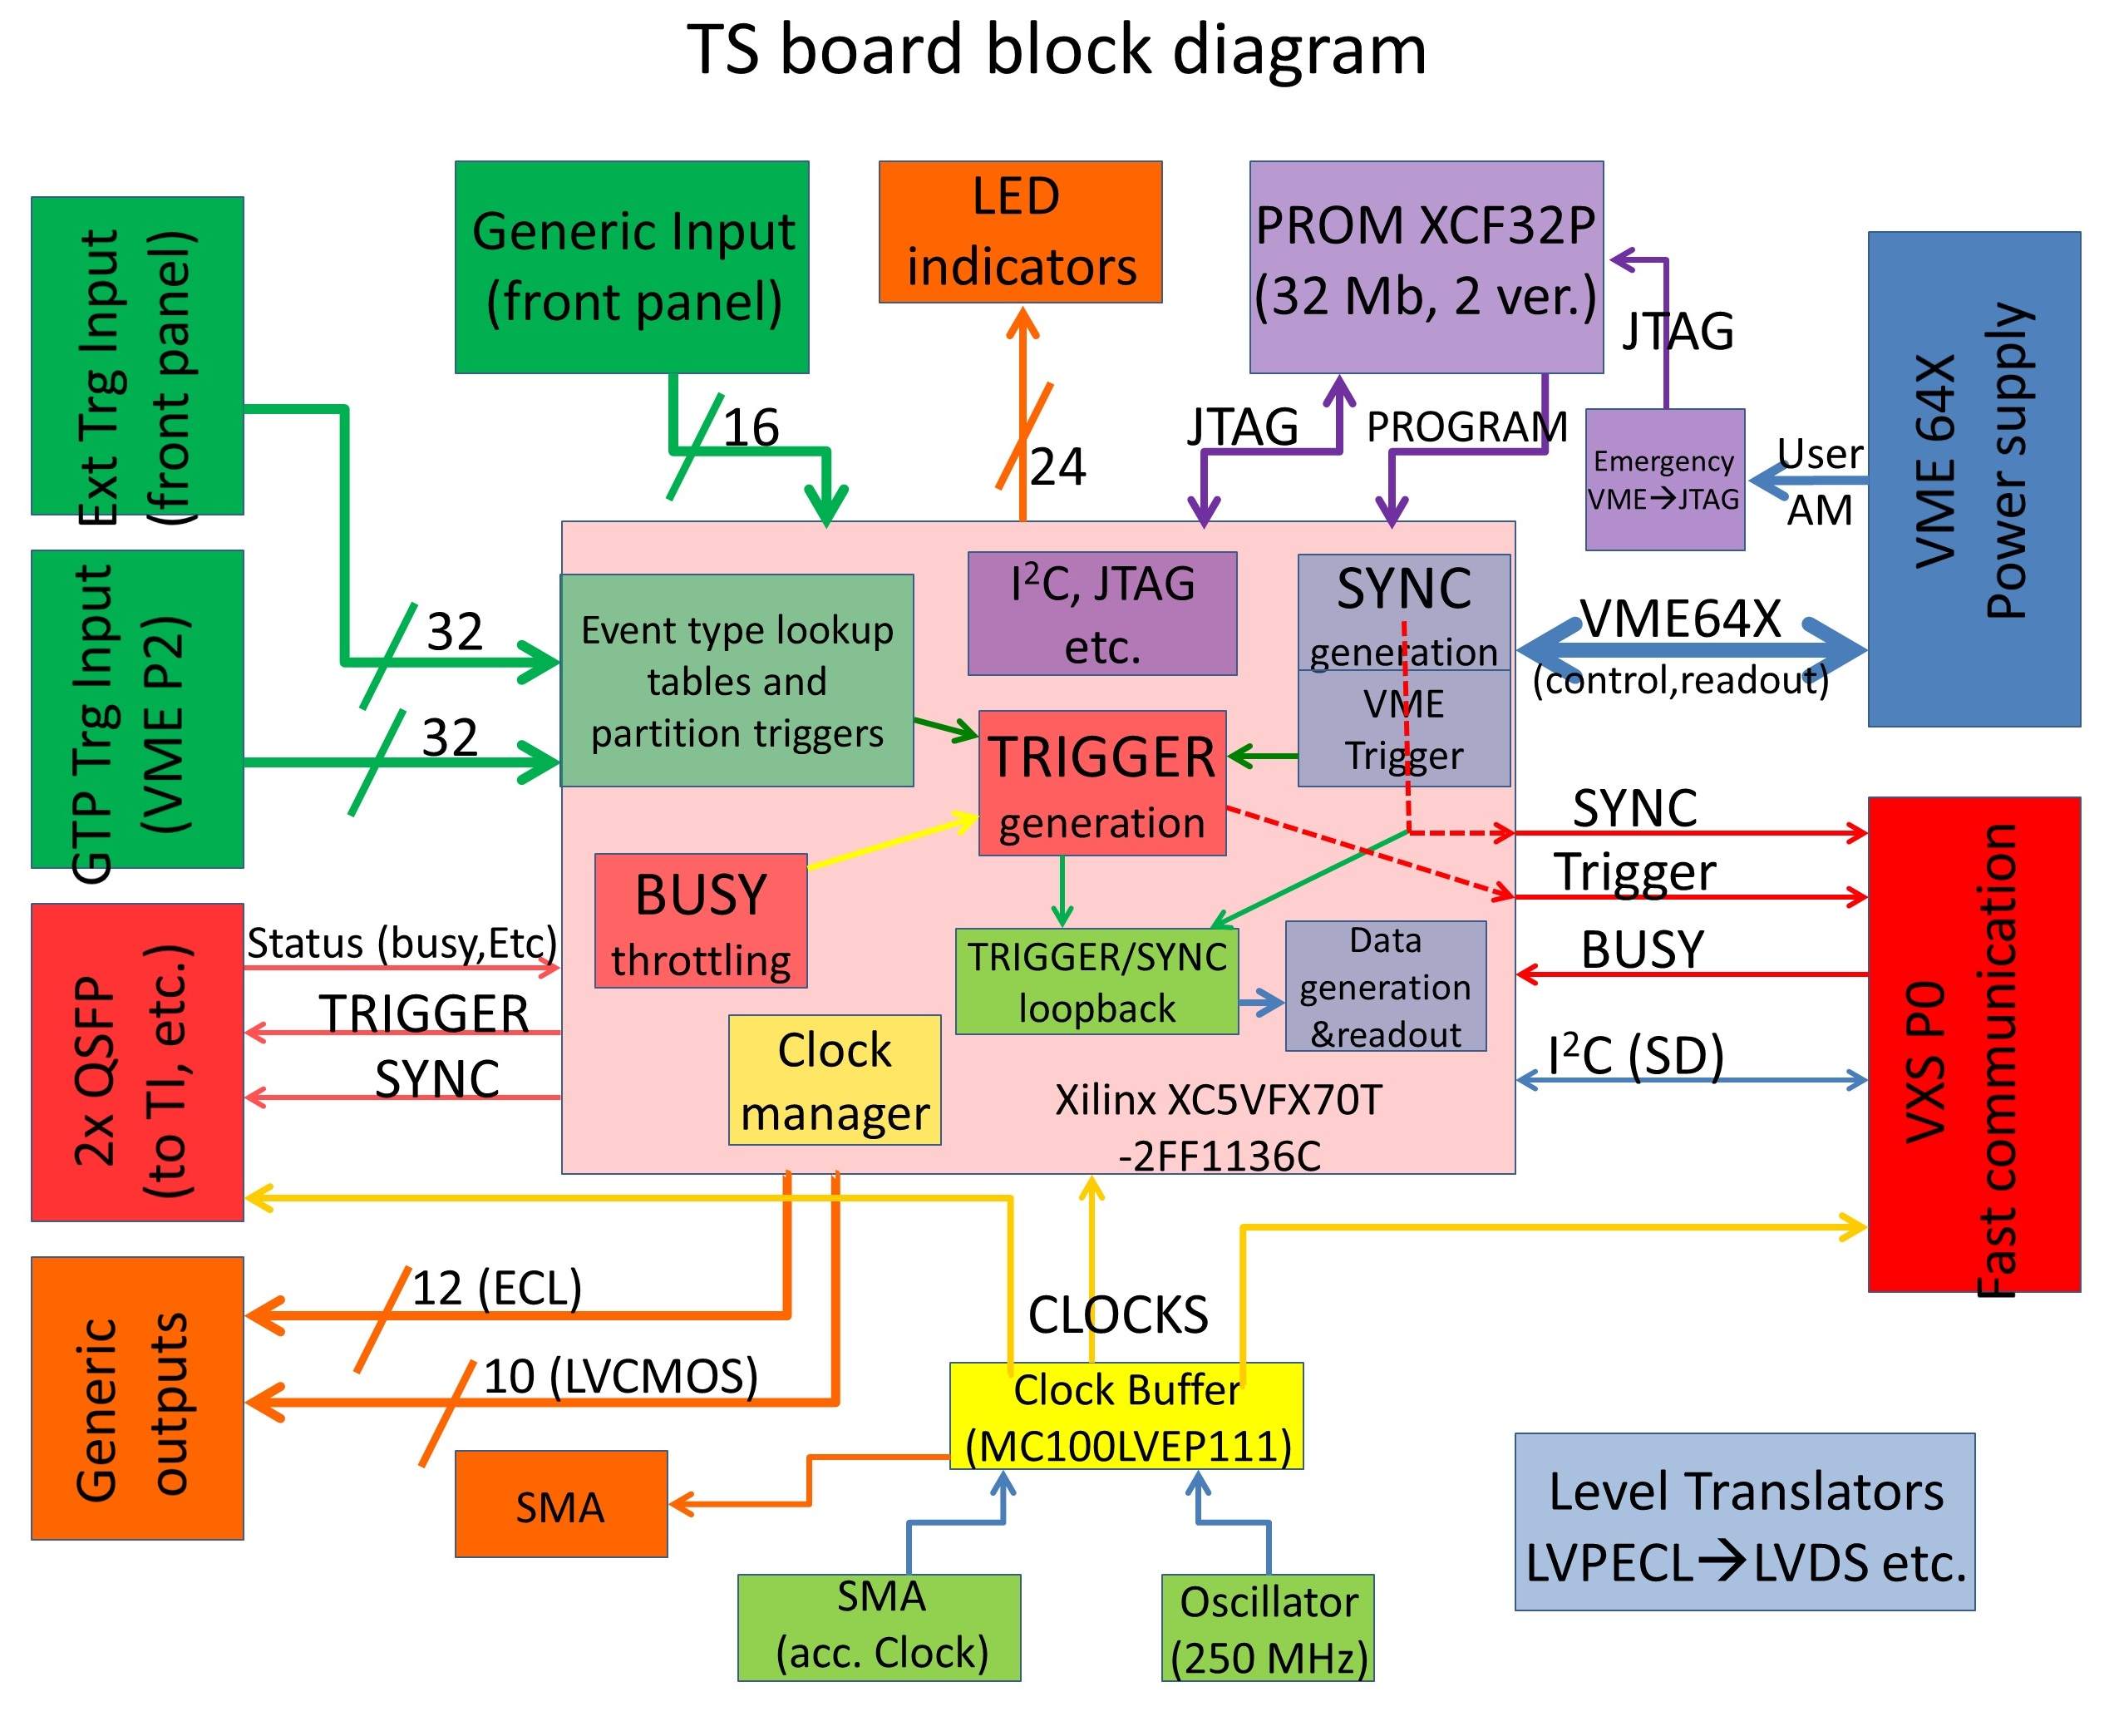
\includegraphics[width=1.0\columnwidth,keepaspectratio]{img/TSdiagram.jpg}
	\caption{TS board diagram.  The TS generates the readout triggers from up to 32 front panel trigger inputs and up to 32 backplane trigger inputs (from GTP), and sends out the triggers via encoded 16-bit words to the backplane.}
	\label{fig:TSdiagram}
\end{figure}

\begin{figure}[hbt]
	\centering
	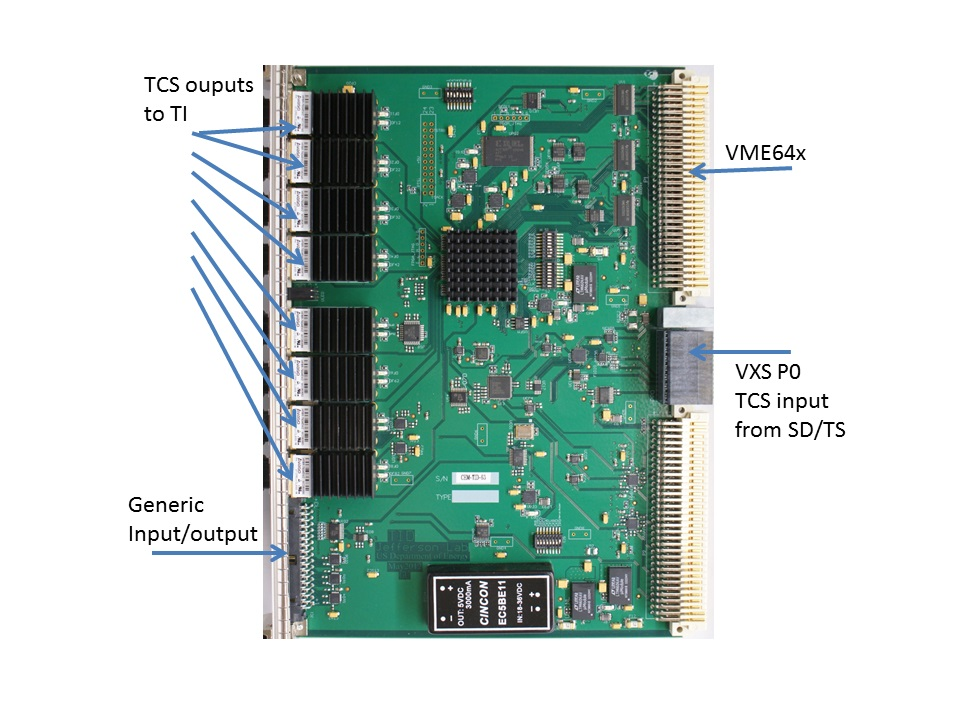
\includegraphics[width=1.0\columnwidth,keepaspectratio]{img/TDused.jpg}
	\caption{Trigger Distribution (TD) board.  The TD board is a 6U by 160mm VME board with VXS connector.  It receives the TCS from TS via the VXS backplane, and distributes the TCS via the front panel QSFP optic links.  It collects the Busy inputs from up to eight TI boards, and generates the readout buffer busies for up to eight front end crates.  The TD sends the collective BUSY to TS to back pressure the trigger generation.}
	\label{fig:TDused}
\end{figure}

\begin{figure}[hbt]
	\centering
	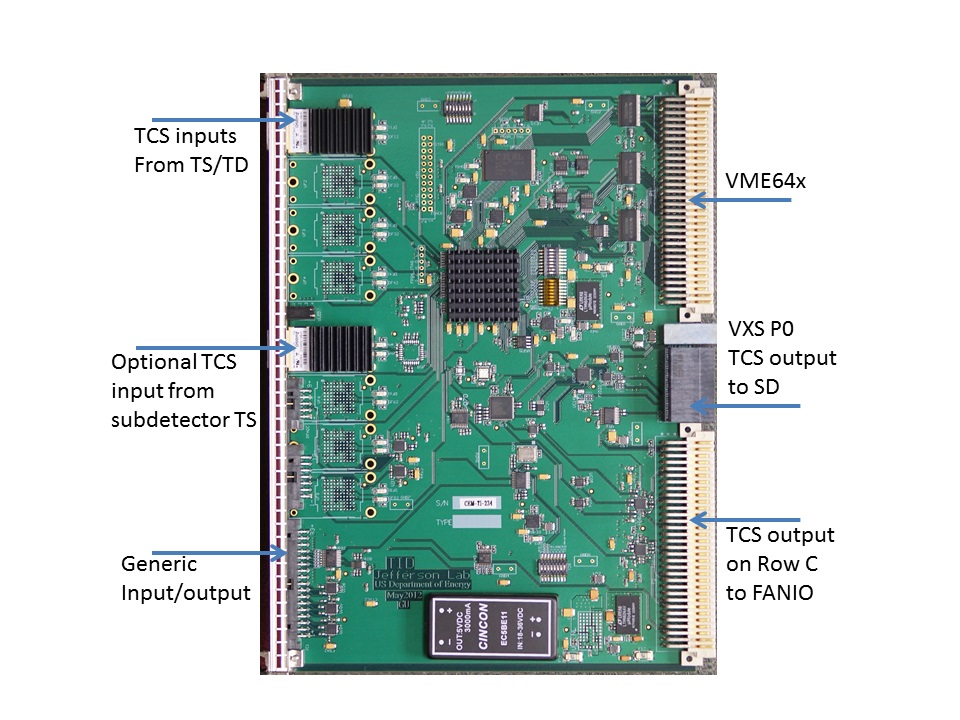
\includegraphics[width=1.0\columnwidth,keepaspectratio]{img/TIused.jpg}
	\caption{Trigger Interface (TI) board.  The TI board is a 6U by 160 mm VME board with (or without) the VXS connector.  It is using the same PCB as TD board with modified components population.  It receives the TCS from TS/TD or a sub-system controller via fiber, and collects the busy and sends to TS/TD via the same fiber.  The TI can also be used as a subsystem controller in the so-called master mode.}
	\label{fig:TIused}
\end{figure}

\begin{figure}[hbt]
	\centering
	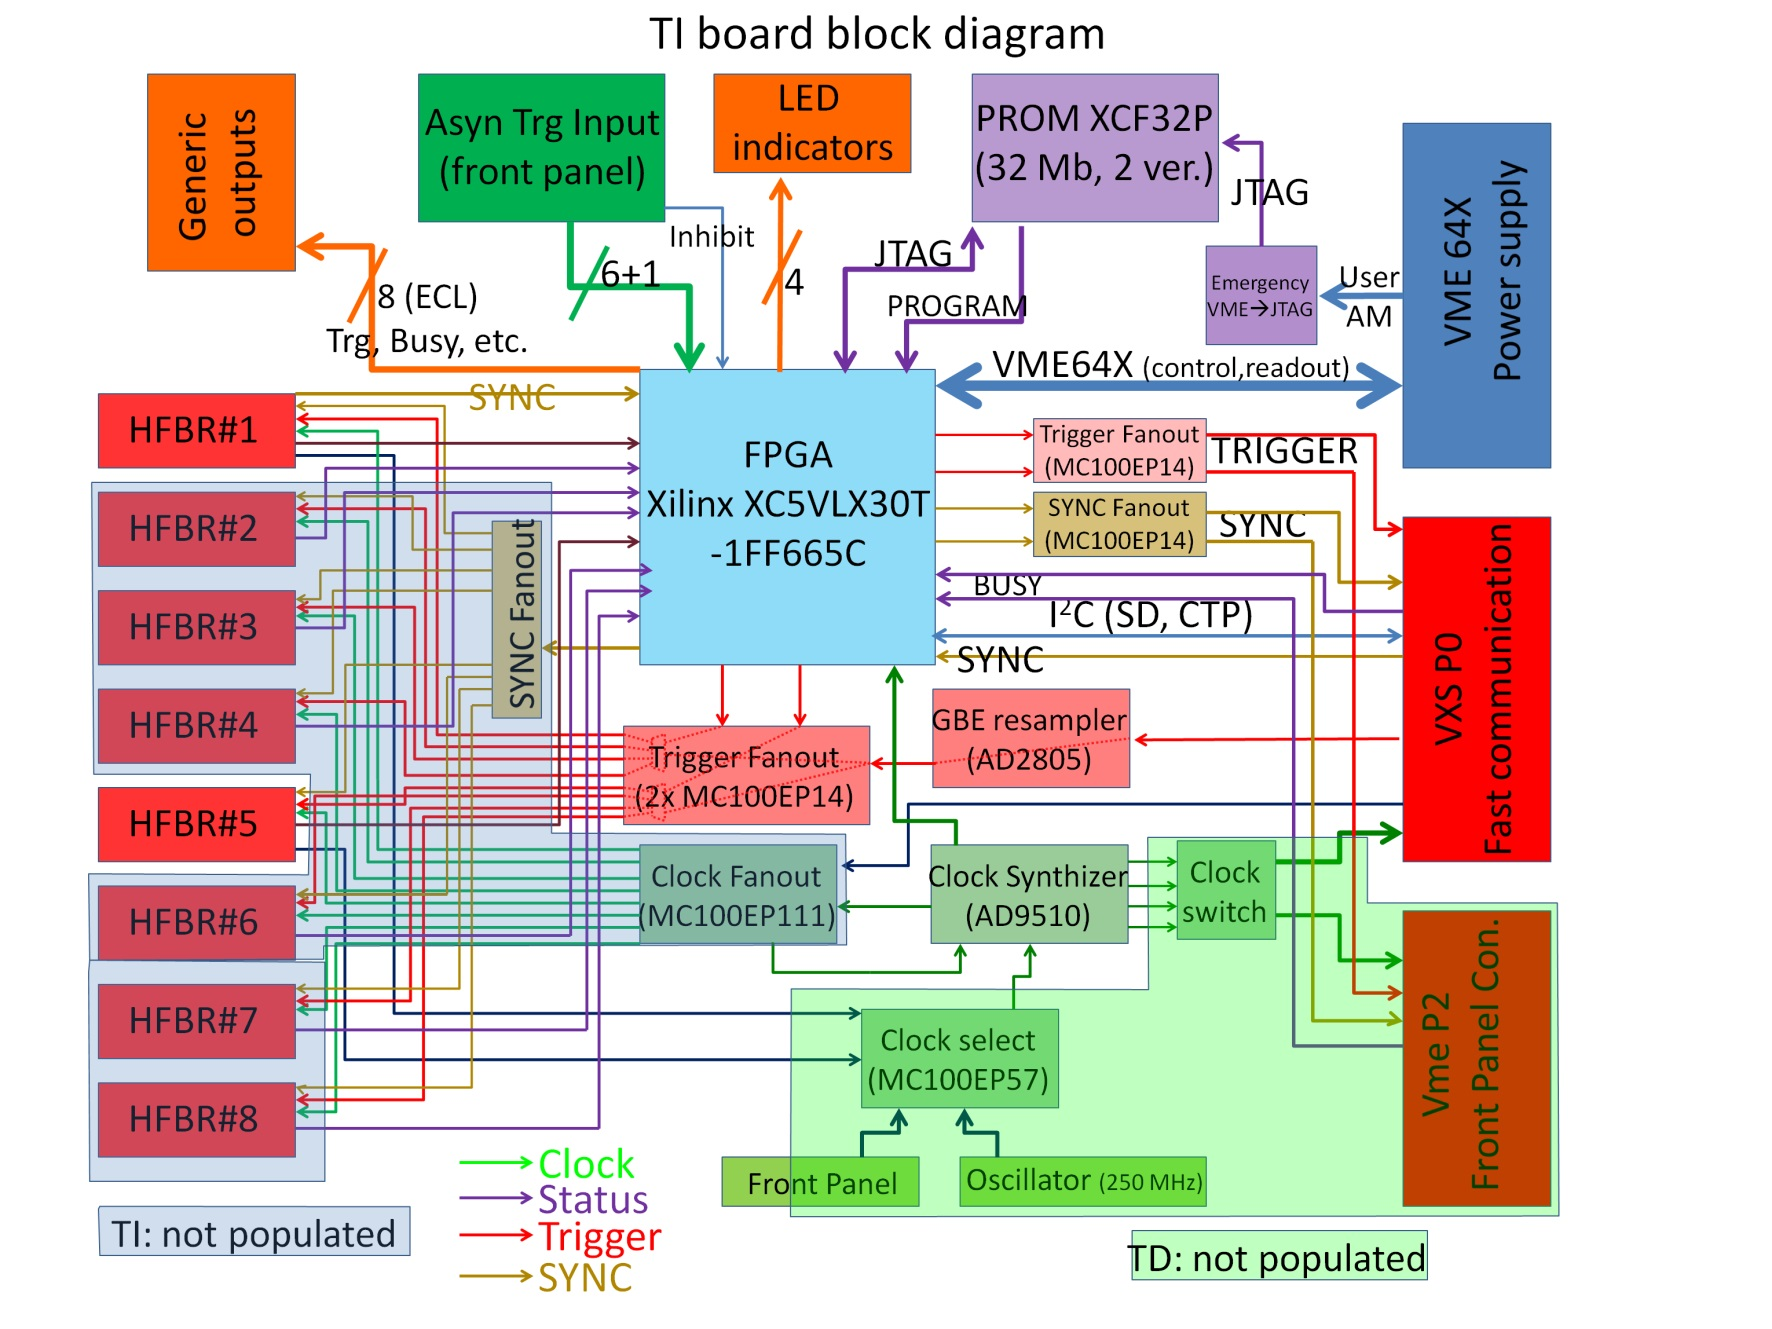
\includegraphics[width=1.0\columnwidth,keepaspectratio]{img/TIdiagram.jpg}
	\caption{TI and TD board diagram.  The TI and TD use the same PCB design, but different component population and FPGA firmware.}
	\label{fig:TIdiagram}
\end{figure}


\subsubsection{Clock Distribution}

The TCS system uses the 250 MHz clock, that comes from the TS in the global trigger distribution crate.  This clock is either generated by the TS on-board oscillator or its fronts panel input.  The clock is fanned out to the VXS P0 connector and then to the SD board.  The SD fans out the clock to the TD boards via the VXS P0 backplane.  The TD boards further fan out to the TI boards via optic fibers.  The TI uses this clock to generate clocks with proper frequencies (250 MHz, 125 MHz, 62.5 MHz, 31.25 MHz and 41.67 MHz) and sends the clocks to the front-end crate SD board, and the SD fans out to the front-end DAQ modules (TDC, ADC).  The fan-out buffer level is minimized on every board to limit the clock jitter.  The slower clocks derived from the main system clock are phase aligned thanks to the Analog Devices AD9510 with a synchronous phase re-alignment command.  The clock jitter is about one ps measured at the front-end electronics.  The clock distribution skew can be adjusted by the SD clock delay if necessary.


\subsubsection{SYNC Distribution}

The TS generates and distributes the SYNC signal.  The SYNC is an encoded 4-bit serialized command transferred at 250 Mbps synchronized with the system clock.  Normally, the serial SYNC line stays at logic high (or ‘1’).  When transferring a SYNC command, the SYNC goes to logic low for one bit, followed by the 4-bit command code.  After the 4-bit SYNC command, the SYNC goes to logic high again.  There is a minimum of four ‘1’s before the next cycle begins.  The SYNC start is phase aligned to the 62.5 MHz clock used for the trigger word transfer, the 41.67 MHz clock used for the CAEN TDC boards, and the 31.25 MHz clock used for Flash ADC boards.  This phase relation is used to synchronize the slower clocks on the TI to the 62.5 MHz clock on the TS.  This also limits the SYNC command to no more than one per 96 ns.  To facilitate the AC coupled optical transceivers, the SYNC is Manchester encoded on the TS and the TD, and Manchester decoded on the TI and the TD.

The SYNC is phase aligned with the 250 MHz system clock on the TI boards using their FPGA’s IODELAY.  The SYNC is synchronized across the TI boards by applying different delays on the individual TI boards.  The delays are determined by the fiber latency measurement.  

The spare fibers between the TD and TI boards are used to measure the fiber latency.  The TI sends a test signal to the TD through one fiber, and the TD loops back the signal through another fiber.  The TI measures the delay between the test pulse and the looped back test pulse using the FPGA counter and the carry chain in the FPGA.  As the fiber skew is small (less than 1 ns for 100 meter fibres), the measurement on these two fibres can be used as the latency of the other fibres in the cable.  
After the SYNC latency compensation, all the TI boards receive the SYNC at the same time with the skew of one system clock period, which is 4 ns.  The synchronized SYNC signals are used to synchronize the triggers as described next.


\subsubsection{Trigger Distribution}

The trigger words, which include the readout trigger signals and event information (event type, trigger timing, etc.), are generated and serialized on the TS.  The serialized trigger word is fanned out by the SD board and the TD board, and deserialized by the TI board.  The 16-bit trigger words are summarized in Table~\ref{tab:trigger_word_definition}.  

\begin{table}
\begin{adjustbox}{width=\columnwidth,center}
	\begin{tabular}{| l | l | l | l |}
		\hline \hline
		Bit 15:12		& 	Bit 11:10 &	Bit 9-0	 & Comment		\\
		\hline
	1001	& Quadrant timing	& Event type	 & GTP major trigger \\
	1010	& Quadrant timing	& Event type	 & Ext major trigger \\
	
	1011	& \multicolumn{2}{c}{Four TS partitions’ event types}    & TS partitioning (4, 3, 2, 1) \\

	\multirow{2}{*}{0110}	& \multirow{2}{*}{Quadrant timing}	& Trigger source & TImaster legacy Trigger \\
		    &                   & Event type	 & (TS) VME trigger     \\
	0101	& Trigger command/Control	& VME command \\
	0100	& TS timer (TS time bit(13:2))	& TI Sync check \\
	0111	& Trigger content	& Additional trigger info \\
		\hline \hline
	\end{tabular}
\end{adjustbox}
\caption{Trigger word definition.  The TS encode the readout trigger, event type, and the fine timing (4ns quadrant) information into a 16-bit word, which is transferred every 16ns.  This 16-bit word can also be some system setting information or the system timer when there is no readout trigger in the 16ns periods.}
\label{tab:trigger_word_definition.}
\end{table}

Both the fiber latency and trigger word serializer/ deserializer are compensated so that all the TI boards send the readout trigger at the same time to the front-end data acquisition electronics.  The SYNC is used in conjunction with a synchronous FIFO to enforce a fixed latency on the trigger distribution. Fig.~\ref{fig:TIsync} shows the diagram of the compensated trigger distribution.

\begin{figure}[hbt]
	\centering
	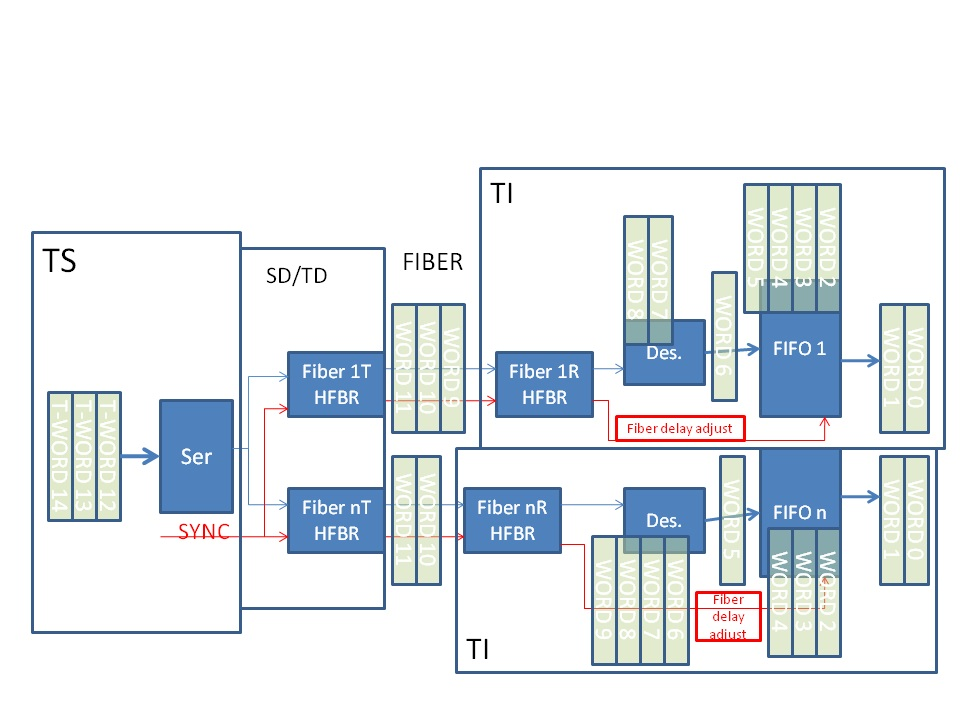
\includegraphics[width=1.0\columnwidth,keepaspectratio]{img/TrgSync.jpg}
	\caption{Trigger synchronization between TIs.  The TI boards delay the decoding of the received readout trigger by the complement of the TS/TD to TI transfer latency, so that all the front end boards receive the readout trigger simultaneously.}
	\label{fig:TIsync}
\end{figure}

On the TI board, the deserialized trigger word is clocked into and clocked out of a FIFO using the 62.5~MHz clock.  At the start-up, the FIFO is reset (0 words) and the FIFO read/write is disabled.  The serial trigger link is idle words only.  On trigger start, the TS starts trigger word transmission.  The TI will write the deserialized data (valid data, that is non-idle data word) to the FIFO.  After some pre-set delay (VME register controlled), the TS issues a ‘Trigger Start’ command on the SYNC link.  When TI receives the ‘Trigger Start’, the TI resets the trigger FIFO readout address, and enables continuous readout of the FIFO.  As the SYNC lines are fiber length adjusted and the 62.5 MHz clocks are phase aligned, the trigger words from the TI board FIFO are synchronized across the system.
The trigger word also has the fine trigger timing information.  By decoding that, the TI board distributes the trigger in 4 ns precision, although the trigger word is serialized every 16 ns.  If the system clock phase is not adjusted, there will be a maximum of 4 ns skew among the clocks on the TI boards, so does the readout trigger.  The clock phase can be adjusted by SD if the skew is critical to the system.


\subsubsection{DAQ synchronization (trigger throttling) control}

Because of the finite memory size and the randomness of the triggers, it is possible for the memory to become overwhelmed somewhere in the system, which could cause DAQ problems.   The TCS throttling mechanism is used to prevent possible memory overflows, and to keep the DAQ synchronized.  Fig.~\ref{fig:DAQ_synchronization} shows the DAQ synchronization logic implementation.  Three methods are used to keep the DAQ synchronized.  These include trigger rules and event limit setting, pipeline DAQ, and synchronization events (special events).

\begin{figure}[hbt]
	\centering
	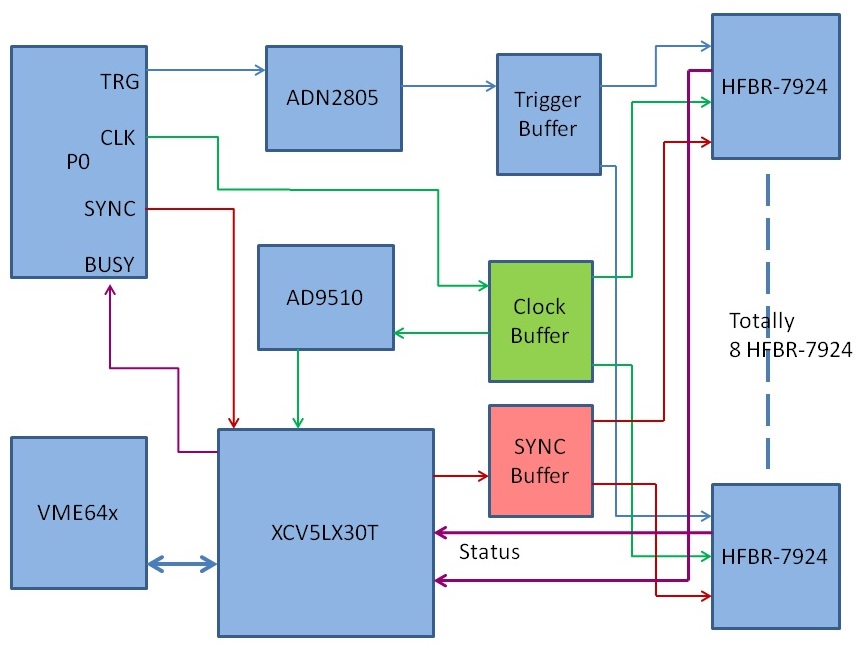
\includegraphics[width=1.0\columnwidth,keepaspectratio]{img/TDdiagram.jpg}
	\caption{DAQ synchronization}
	\label{fig:DAQ_synchronization}
\end{figure}


%REFERENCES
%[1] 	J. Gu etal. (2014, May). The TRIGGER/CLOCK/SYNC Distribution for TJNAF 12 GeV Upgrade Experiments    %https://coda.jlab.org/wiki/index.php/Trigger_distribution_overview
% [2] 	J. Gu. Description and technical information for the Trigger Supervisor (TS) module.  TJNAF, VA, 2013.  %Available: https://coda.jlab.org/drupal/system/files/pdfs/HardwareManual/TS/TS.pdf 
%[3] J. Gu, etal, 	“Design of the Trigger Interface and Distribution Board for TJNAF 12 GeV Upgrade,” IEEE Trans. Nucl. %Sci., Vol. 60, no. 5, pp 3714-3719, Oct. 2013

	
\subsection{Signal Distribution Module (SD)}

The Signal Distribution Board (SD \cite{sd-ref}) module (see Fig.~\ref{fig:SDpic}) occupies the “B” switch card slot as specified in VITA 41. The main purpose of this module is to distribute the signals received from payload slot 18 (Trigger Interface board) of a VXS crate to the 16 other payload slots (ADC boards).

The SD module distributes the 4 LVPECL differential pair  signals from payload slot 18 to 16 VXS payload slots within the crate. This is done using the high-speed, point-to-point connections from the switch slot to each payload slot. The four distributed signals are length-matched to minimize the output jitter seen on all of the payload slots. Three of the four remaining pairs are LVDS signals routed from the each payload module to the FPGA on the SD module. The last pair is an LVDS signal routed from the FPGA on the SD module to each payload module. Each of the 16 payload modules has a single-ended signal to the SD module and one from the SD module back to the payload module.

\begin{figure}[hbt]
	\centering
	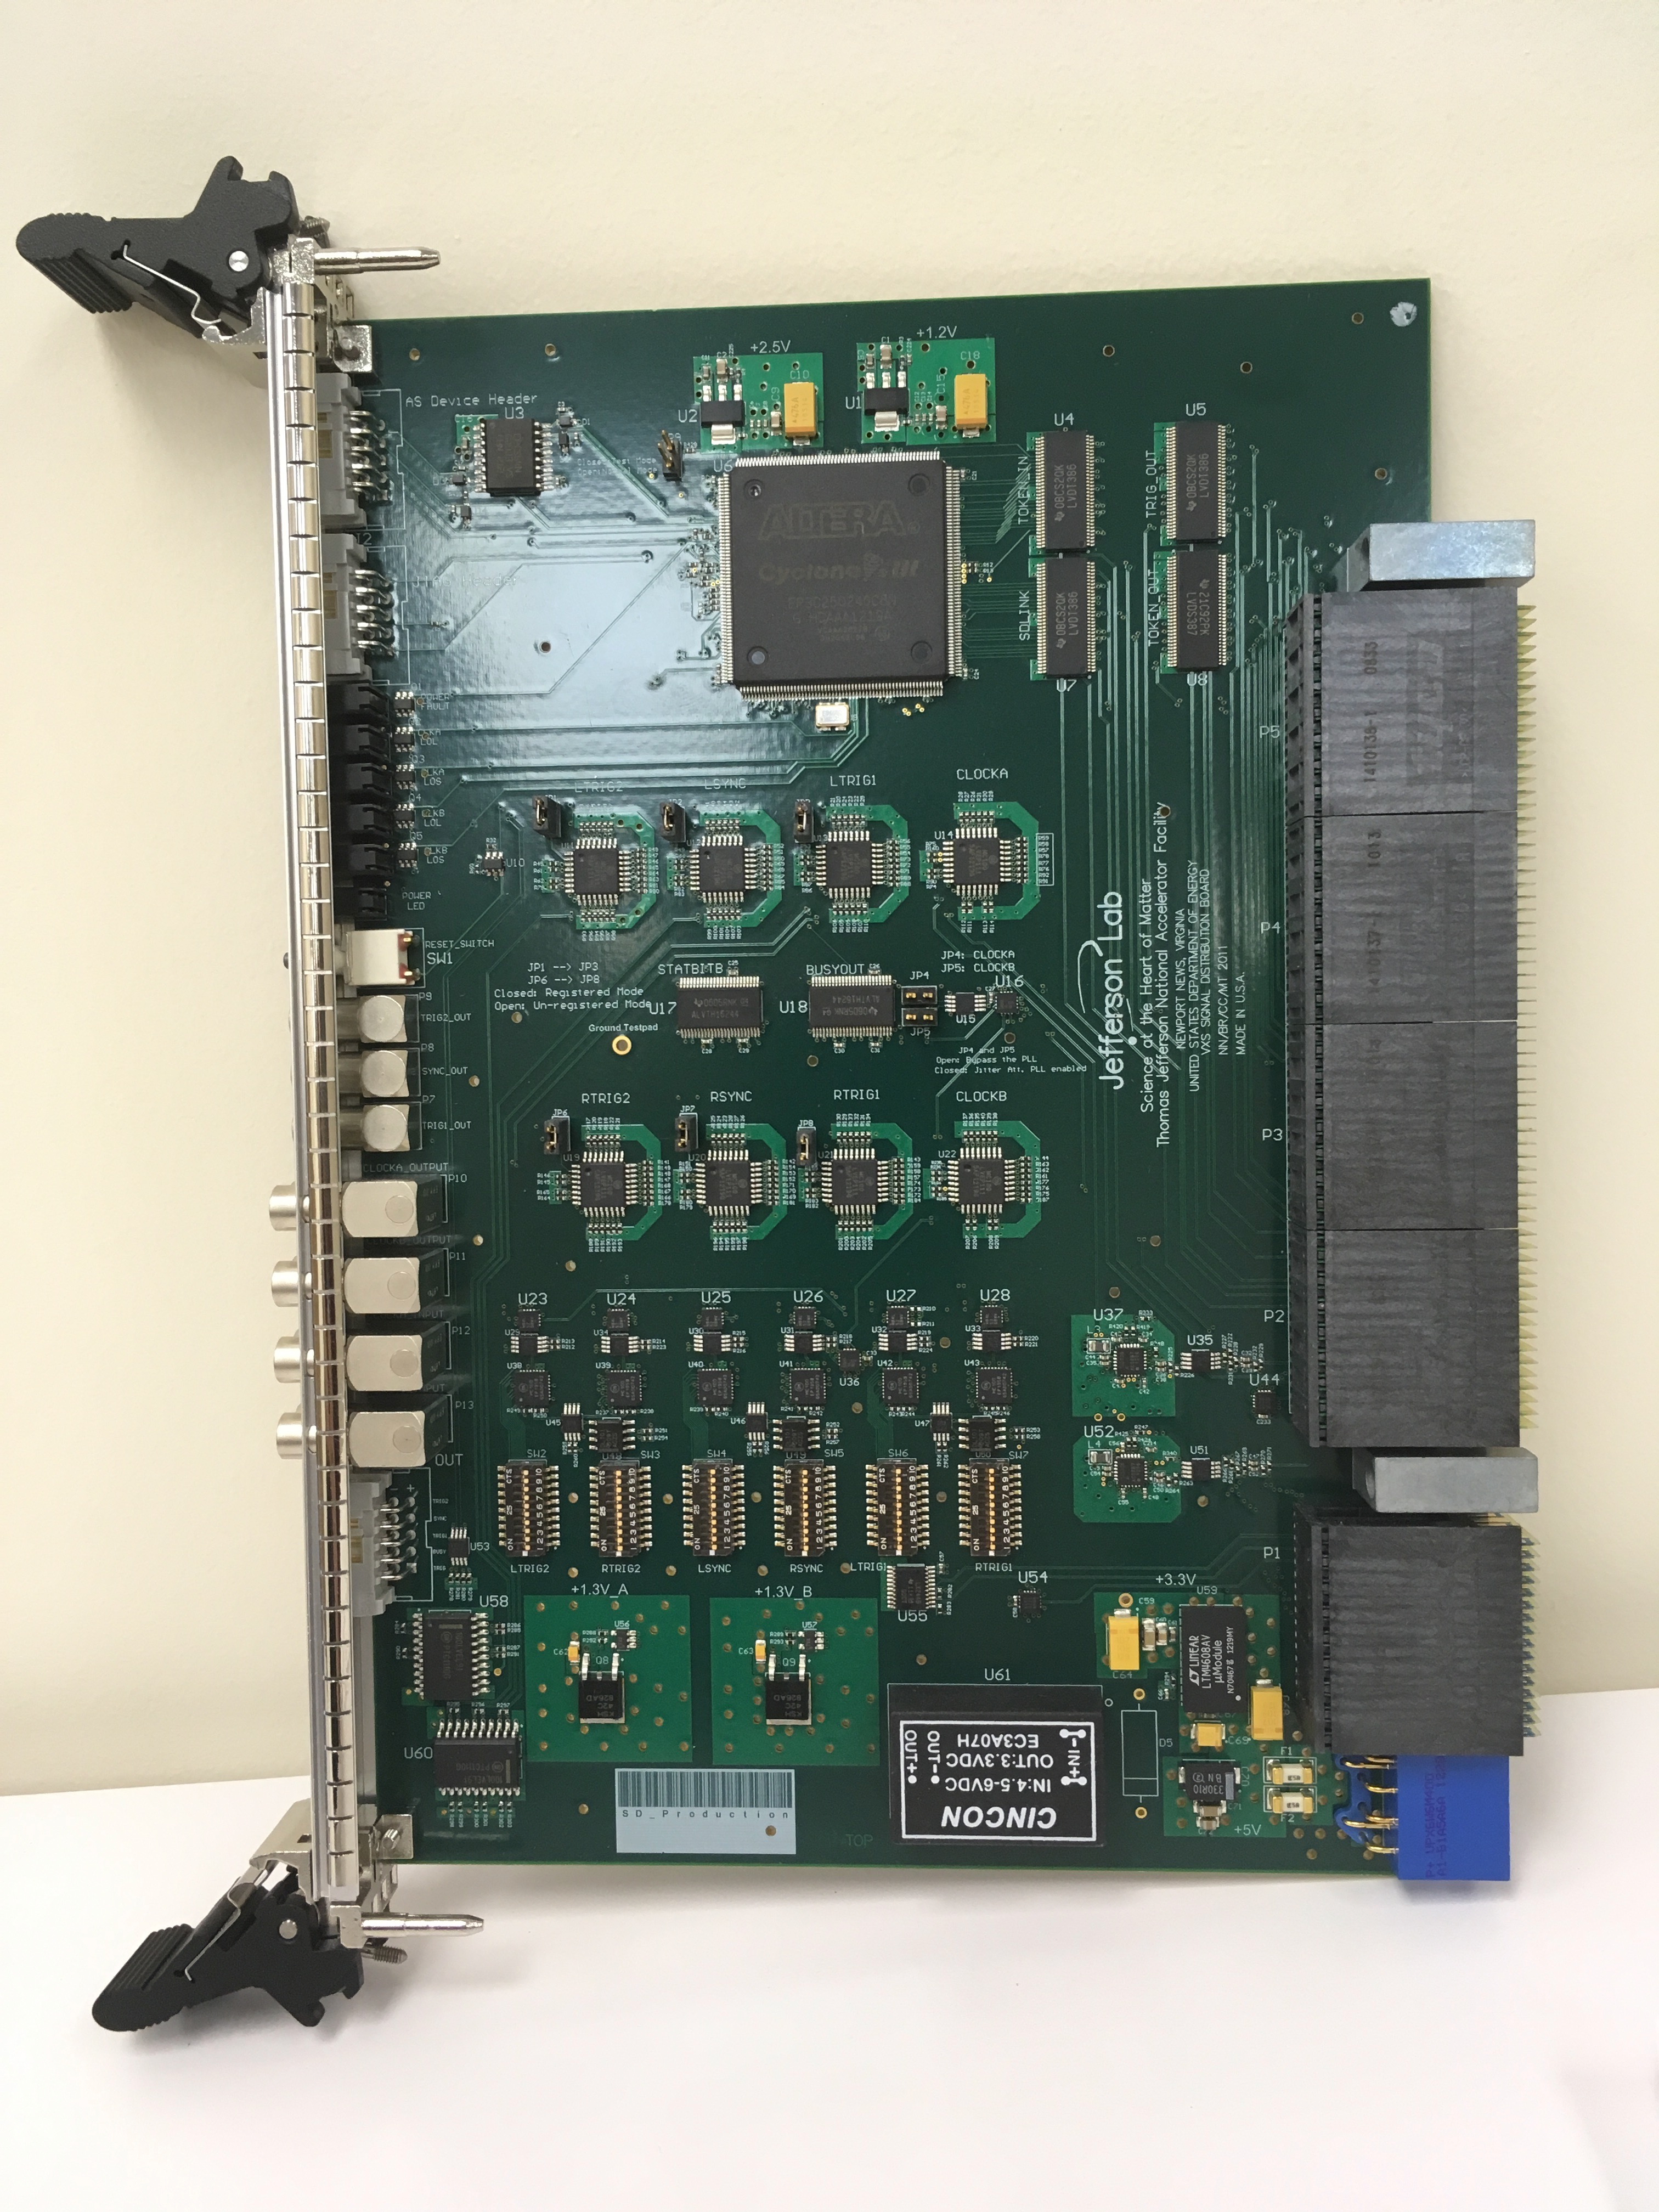
\includegraphics[width=1.0\columnwidth,keepaspectratio]{img/sd_board.jpg}
	\caption{Signal Distribution module (SD)}
	\label{fig:SDpic}
\end{figure}


\subsection{Flash ADC Module (FADC250)}

A 16-channel 250 MSPS pipelined flash ADC (FADC \cite{fadc-ref}, see Fig.~\ref{fig:FADC250pic}) with 12-bit precision was designed to digitize and process detector pulses for experiments at JLab.  The FADC250 module (see Fig.~\ref{fig:FADC250_board}) conforms to the VITA-41 VME64x switched serial (VXS) standard.  Each channel of the module accepts input signals on a LEMO style coaxial connector and has three user-selectable ranges (0.5 V, 1.0 V, 2.0 V).  Differential signal conditioning scales the input signals to within the dynamic range of the ADC and a single-pole low pass filter limits the signal bandwidth to the Nyquist band of the converter (125 MHz). Individual channel offsets are accomplished by means of DACs under VME control.  Each channel has its own dedicated ADC chip (Analog Devices AD9230). Both positive and negative polarity input signals are supported. The 250 MHz clock is distributed to the ADC chips through a low jitter ($<$ 2~ps) network.  

\begin{figure}[hbt]
	\centering
	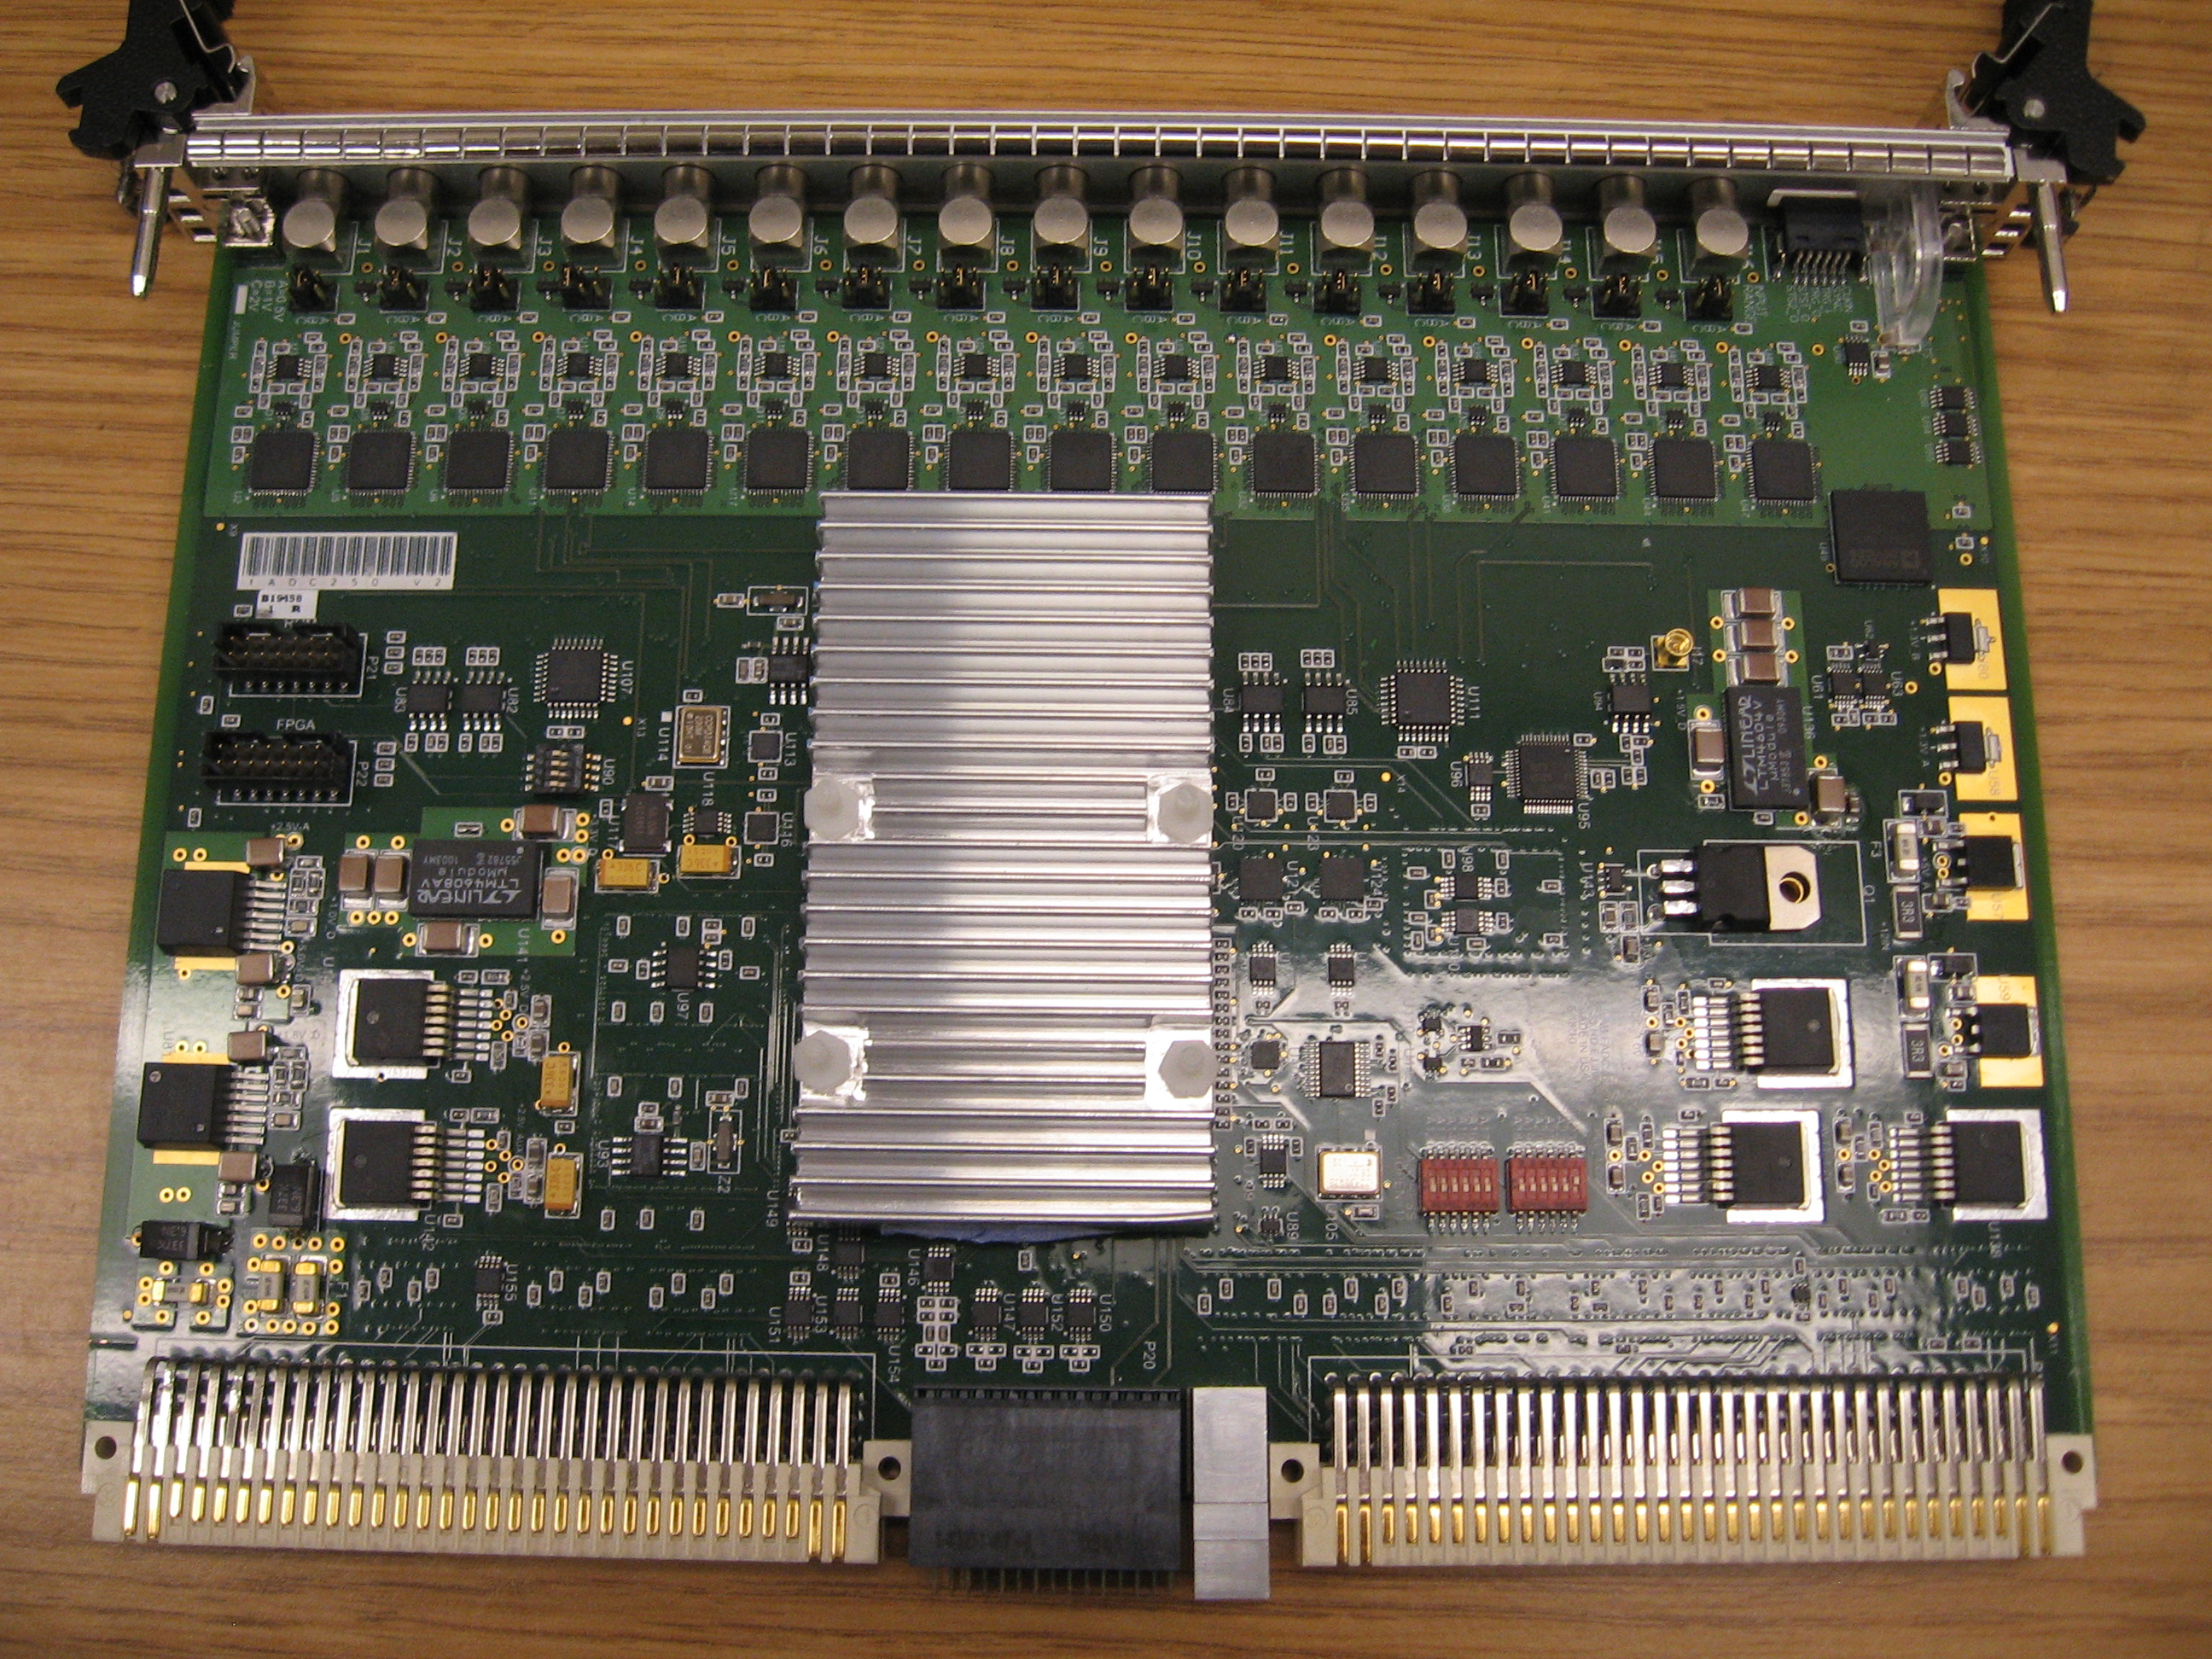
\includegraphics[width=1.0\columnwidth,keepaspectratio]{img/FADC250pic.jpg}
	\caption{Flash ADC module (FADC250)}
	\label{fig:FADC250pic}
\end{figure}

\begin{figure}[hbt]
	\centering
	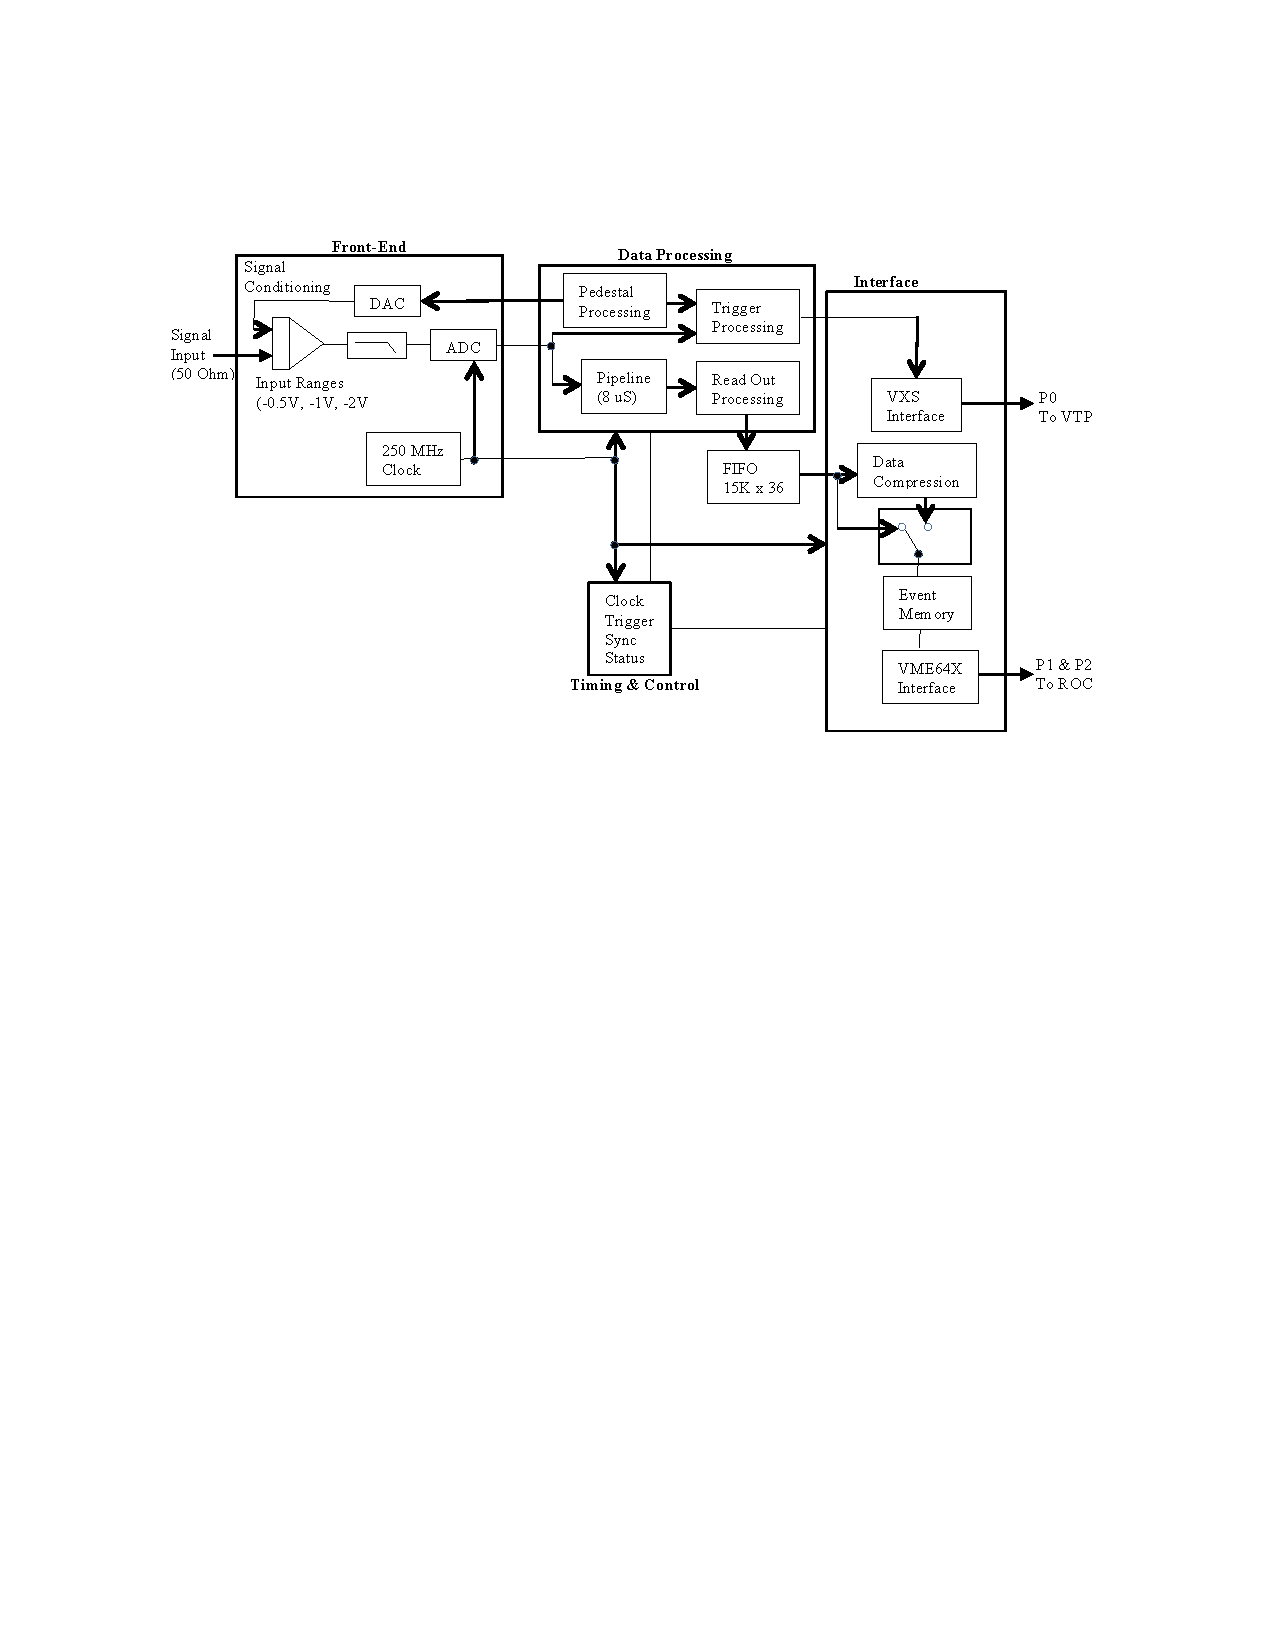
\includegraphics[width=1.0\columnwidth,keepaspectratio]{img/FADC250_Diagram.pdf}
	\caption{Flash ADC module diagram (FADC250)}
	\label{fig:FADC250_board}
\end{figure}

Digitized data from the 16 FADC chips is processed and formatted for readout in a pair of high performance Xilinx FPGAs. The digitized data from the ADCs follows two distinct paths.  Logic in the trigger data path pre-processes data for the trigger algorithms of the VXS Trigger Processor (VTP). The FADC250 module continuously streams this data to the crate VTP located in VXS switch slot A via high-speed serial links of the VXS fabric.  Data from multiple VTPs and other modules are used to form a global trigger signal that is returned to the crates to initiate data readout.

The readout data path continuously stores digitized data for each channel in circular buffers. When a trigger signal is received by the module a programmable window up to 2 $\mu$s wide of digitized data is extracted from the buffers for processing. The starting point of this window can be programmed up to 8 $\mu$s earlier than the arrival of the trigger signal to account for the time required to form the trigger signal.  Zero suppression on the extracted data may be implemented for each channel using programmable thresholds.  A lossless data compression algorithm can also be applied to the data of each channel with typical compression factors of 2 to 3. The design is pipelined so that data from multiple triggers can be processed simultaneously.  Triggers separated in time by as little as 50 ns can be accepted by the module. The trigger number and trigger time (clock periods since last synchronization) are reported along with the channel data so that data from multiple modules can be correctly assembled into events. 

Data associated with a programmable number ``N'' of triggers is packaged into a block of data for read out over VME.  ``N'' can take values from 1 to 255, with 40 being a typical value chosen.  Data is stored in an on-board 8 MB SRAM as 64-bit words to match the 64-bit high-speed (200 MB/s) dual edge VME Source Synchronous Transfer (2eSST) mode employed to read out the module.  

In order to save the overhead of setting up a DMA transfer for each FADC250 module in the crate, a chained block readout mechanism with token passing is used.  A common address range is enabled for all modules in the crate but only the module having the token will respond to a read request.  A single logical DMA read is initiated by the VME crate controller and the first module in the chain supplies data from its block of event fragments.  When the block data from the first module is exhausted, a token signal is passed to the next module in the chain and this module then proceeds to transmit its data from its block.  When the block for the data from that module is exhausted, it transfers the token to the next module.  This continues until the data from the last module in the chain is exhausted.  Instead of passing the token the last module asserts the VME bus error signal (BERR), which terminates the DMA cycle.  The user returns the token to the first module and the process can begin again when the next block of events is ready for readout.  The user does not have to query the modules in advance to discover the number of words to read out.  The DMA is set up with a total number of words larger than any expected value for the entire crate.  Data from each module is tagged with the slot number to identify its source.  The token passes along a VXS signal line to VXS switch slot B, where a module there (SD) routes it to the next enabled module.


\subsection{Discriminator Scaler Module (DSC2)}

The Discriminator Scaler Module (DSC2 \cite{dsc2-ref}, see Fig.~\ref{fig:dsc2_board}) is a 16-channel general purpose discriminator and scaler module designed as a 6U VME card. It replaces an older design, improving on jitter, noise, crosstalk, and adding new features.

\begin{figure}[hbt]
	\centering
	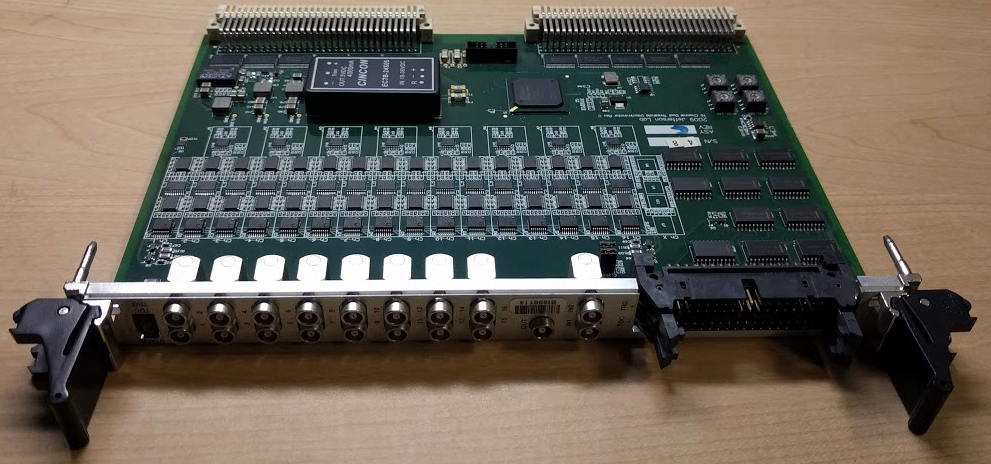
\includegraphics[width=1.0\columnwidth,keepaspectratio]{img/dsc2_board.png}
	\caption{Discriminator Scaler module (DSC2)}
	\label{fig:dsc2_board}
\end{figure}

\begin{center}
	DSC2 Specifications\\
	\begin{tabular}{| l | l |}
		\hline \hline
		Property			& Value				\\
		\hline
		{\bf Analog Discriminator}	&				\\
		Threshold			& 0 to -1023 mV			\\
		Pulse width			& 4 ns to 40 ns			\\
		Dead-time			& 4 ns typ. w/8 ns pulser width	\\
		Maximum input rate		& $>$125 MHz 			\\
		Ch-ch isolation			& $>$65 dB			\\
		Threshold noise			& 1.3 mV RMS (typical)		\\
		Slew-rate delay disperson	& $<$20 ps			\\
		Input-to-output delay		& $<$5 ns			\\
		{\bf Digital Processing}	&				\\
		Digital delay step		& 4 ns				\\
		Digital delay maximum		& 1 us				\\
		Digital width maximum		& 1 us				\\
		Maximum count rate		& 125 MHz			\\
		\hline \hline
	\end{tabular}
\end{center}

\paragraph{Discriminator}
Inputs are single-ended LEMO and leading-edge discrimated by two different thresholds. Typically one threshold is used for time-to-digital applications and the other threshold is used for trigger applications. There are separate differential ECL outputs for each channel and threshold. Low jitter performance was an important goal of the design as this module will be used in high resolution applications. Fig.~\ref{fig:dsc2_jitter} shows the typical jitter as a function of a variety of input slew rate signals and threshold overdrive conditions.

\begin{figure}[hbt]
	\centering
	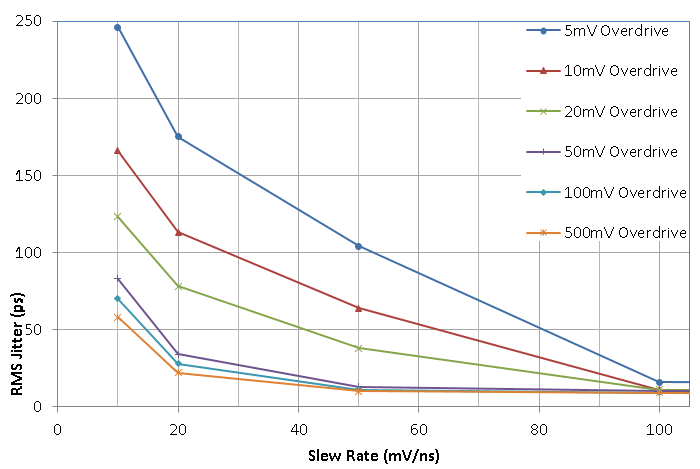
\includegraphics[width=1.0\columnwidth,keepaspectratio]{img/dsc2_jitter.png}
	\caption{Output Jitter vs Input slew rate and overdrive}
	\label{fig:dsc2_jitter}
\end{figure}

\paragraph{Digital Processing}
A Xilinx Spartan 3A FPGA is used to implement the VME interface, scalers, discriminator controls, and scaler event building features. Each channel and threshold has two scalers associated with it. The first scaler counts all threshold crossings for the input. The second scaler is gated using a front-panel input source, which can be useful to computing dead-time of channels and many other applications. Additionally, reference scalers are accumulated (a gated and ungated version) that count the elapsed time, which can be used to normalize inputs scalers to Hz. All together there are 68 scalers, which can be slow to read over VME if using single-cycle transfers. An event builder is implemented that can synchronously read (and optionally clear) all scalers and build an event with this data. Over 100 events can be buffered and readout using the VME 2eSST protocol at 200~MB/s.


\subsection{TDC Modiles (v1190/v1290)}

Commercial CAEN V1190/V1290/V1290N TDC \cite{tdc-ref} boards are used for timing measurements in the PMT-based CLAS12 detectors (see Fig.~\ref{fig:v1190_board}). The V1190 has timing resolution about 100~ps and the V1290 about 35~ps. All boards installed in CLAS12 run on an external 250/6=41.666~MHz clock rather then internal 40~MHz clock. The use of a different clock required compensation table remeasuring and reloading.

\begin{figure}[hbt]
	\centering
	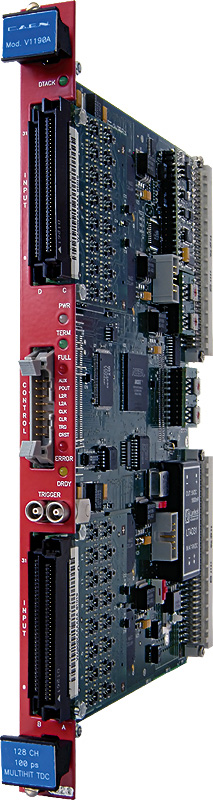
\includegraphics[width=0.2\columnwidth,keepaspectratio]{img/v1190_board.jpg}
	\caption{CAEN V1190 TDC module (V1190)}
	\label{fig:v1190_board}
\end{figure}

\subsection{Drift Chamber Readout Board (DCRB)}

\begin{figure}[hbt]
	\centering
	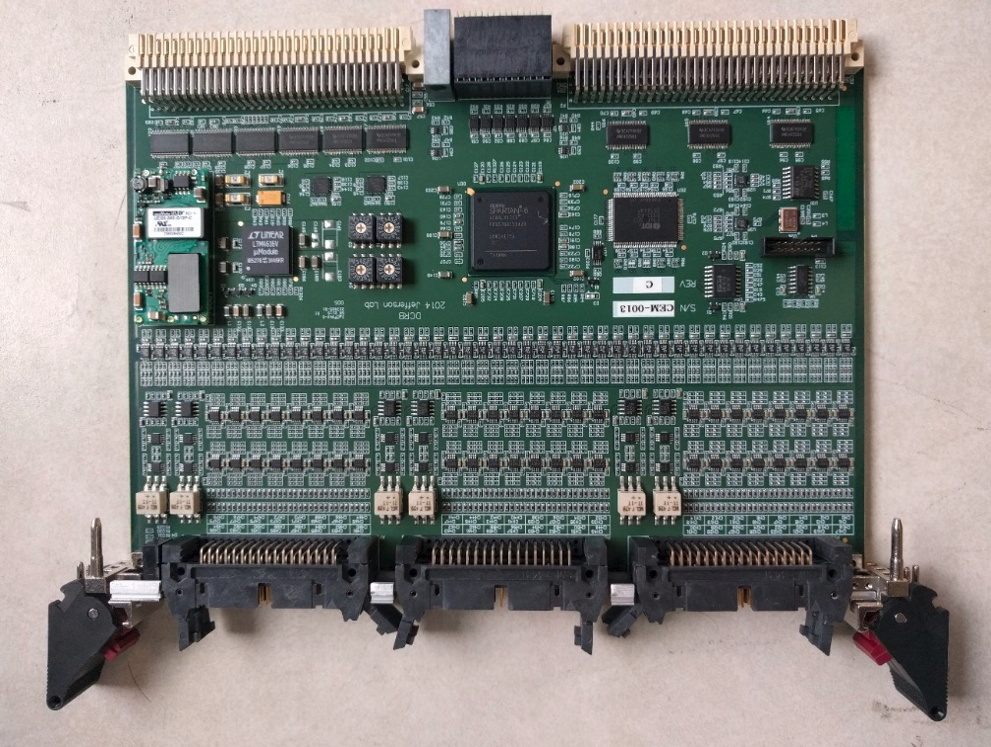
\includegraphics[width=1.0\columnwidth,keepaspectratio]{img/dcrb_board.png}
	\caption{Drift Chamber Readout Board (DCRB)}
	\label{fig:dcrb_board}
\end{figure}

The Drift Chamber Readout Board (DCRB \cite{dcrb-ref}, see Fig.~\ref{fig:dcrb_board}) is a 96-channel amplifier, discriminator, and time-to-digital converter module used to digitize and readout hits from the CLAS12 Drift Chambers. A single VXS crate of DCRB modules can readout a full region of the drift chambers for a single sector resulting in 18 VXS crates of DCRBs to instrument 6 sectors each having 3 regions of drift chamber.

\paragraph{Analog Inputs}
Each DCRB receives 96 differential analog signal pairs using twisted pair cabling from the drift chamber pre-amplifiers. The pre-amplfiers located on the detector provide a gain of ~2.3~mV/$\mu$A. On the DCRB each analog input channel is amplified by a voltage gain of 30 and then discriminated by a programmable threshold (common to all channels on the board with an effective chamber wire threshold range of 0 to 3.5/$\mu$A).

\paragraph{TDC Event Builder}
All discriminated channels go to a Xilinx Spartan 6 FPGA where a 96-channel 1~ns resolution time-to-digital converter (TDC) is implemented in firmware. The TDC is based on the ISERDES2 shift register FPGA primitive that directly samples of the digital input with a single-data-rate (SDR) input register clocked at 1~GHz. The TDC sampling clock is synchronized to the CLAS12 master oscillator, making it easy to relate hit times in the drift chamber to the other detectors in CLAS12. The TDC inputs are buffered to support multiple hits, allowing for an average hit rate of 4~MHz per input before loss of data, which exceeds the chamber design hits rates by a few orders of magnitude. Hits from groups of 16 channels are written into a large buffer that a linked-list content addressable memory (CAM) tracks for 16~$\mu$s. When a L1A trigger signal is received, a time window of hits is extracted from the TDC hit buffer. The readout window times are supplied to the CAM, and the CAM provides the address of the last hit matching each readout time bin. The hit buffer is then read to extract the hit and also the address of the next hit in the buffer matching the time bin (this is the linked list behavior). The result is an extremely fast event builder with natural zero suppression that does not require time sorted data. Cleanup is accomplished by a timer that invalidates the CAM entries after time bins are older then 16~$\mu$s. Hits for an event are assembled and buffered in a 2~MByte external RAM, which is readout through the VME bus using the 2eSST protocol at 200~MB/s.

\paragraph{Calibration Support}
A programmable amplitude pulse generator is implemented that can inject test pulses directly into the DCRB differential amplifier inputs as well as to the pre-amplfiers that are on the detector. This provides a way to test points of failure, check channel gain, and check channel delays without any extra equipment. A scaler is implemented on each channel for slow control monitoring of all chamber wires.

\subsection{VXS Silicon Readout Module (VSCM)}
The CLAS12 Silicon Vertex Tracker detector (SVT, \cite{svt-ref}) front-end utilizes the data driven FSSR2 ASIC for digitization. The VXS Silicon Readout Module (VSCM \cite{vscm-ref}, Fig.~\ref{fig:vscm_board}) was designed to interface the FSSR2-based front-end to the CLAS12 DAQ system. This system is capable of reading out all 33,792 SVT channels in 3 VXS crates.

\begin{figure}[hbt]
	\centering
	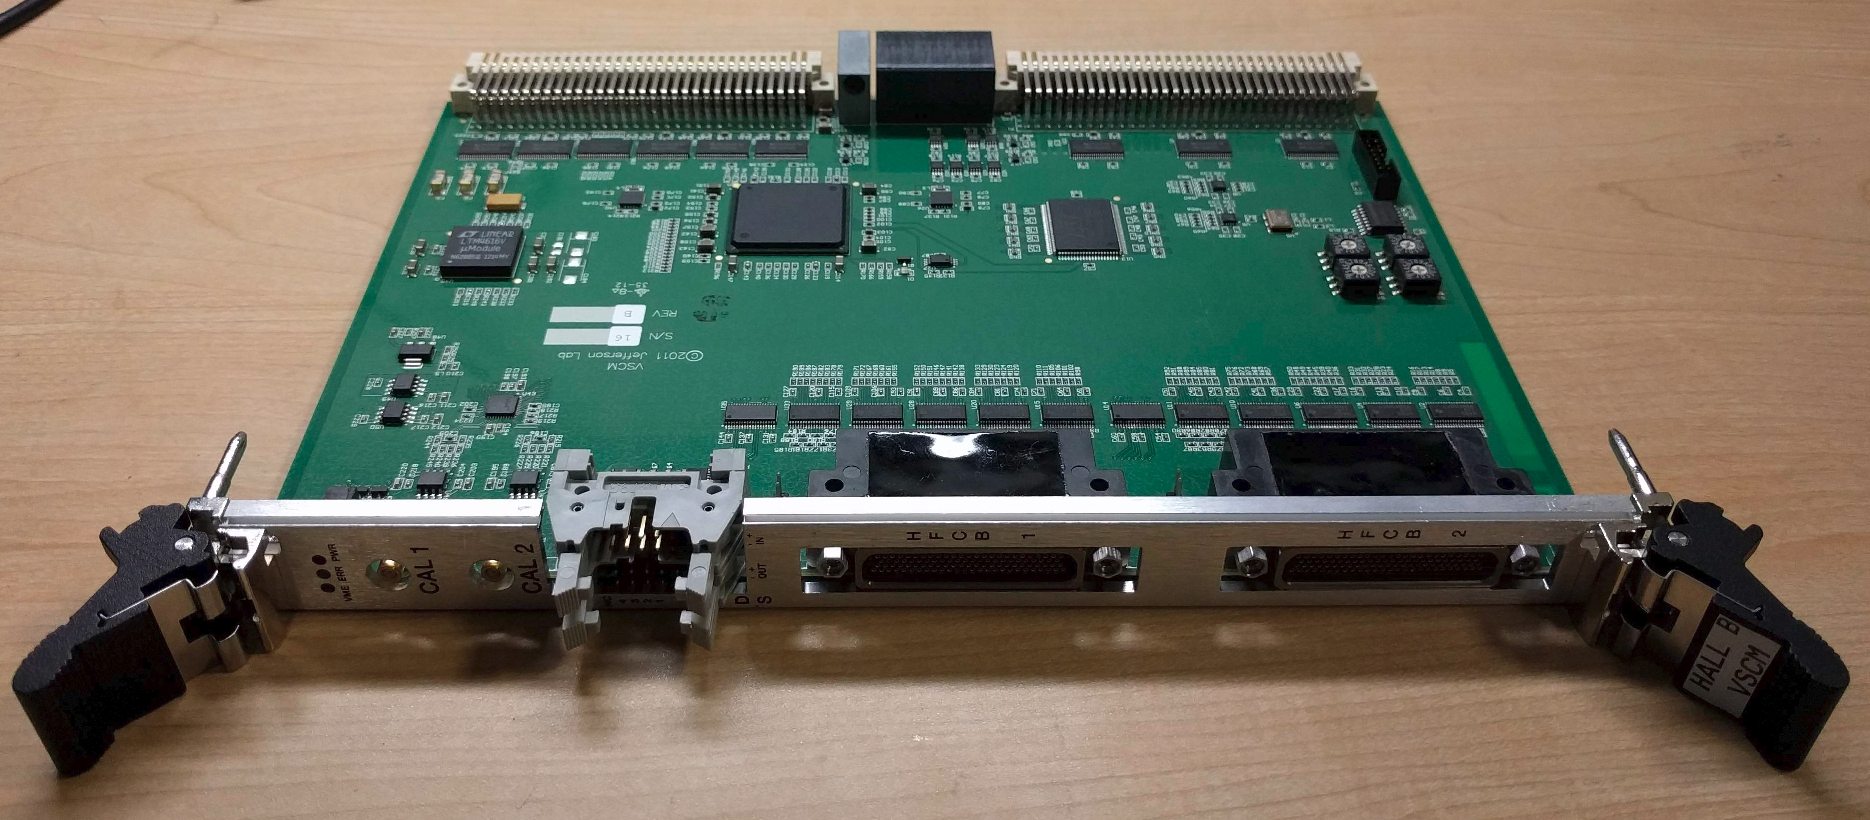
\includegraphics[width=1.0\columnwidth,keepaspectratio]{img/vscm_board.png}
	\caption{VXS Silicon Readout Module (VSCM)}
	\label{fig:vscm_board}
\end{figure}

The main features of the VSCM include:

\begin{itemize}
	\item Receives 8 FSSR2 streams, each at 840~Mbps
	\item De-randomizes hits into an 8~$\mu$s buffer
	\item 512k hit, multi-event buffer
	\item Supports $>$1~MHz trigger rate
	\item Programmable amplitude charge injector
	\item 1~ns resolution time-to-digital converter (TDC)
	\item Per channel hit scaler
	\item FSSR2 synchronization, status, and control
\end{itemize}

\paragraph{Event Builder}
The VSCM deserializes the FSSR2 streams, checks for errors, and decodes the hits, which are stored in an 8~$\mu$s circular memory. The hits are not guaranteed to be time ordered, so the timestamp and channel number are used to form the circular memory address (rather than storing in the order received). The VSCM also implements an 8-channel 1~ns time-to-digital converter (TDC) that measures the logic OR of hits from each FSSR2 ASIC. This high time resolution is significantly better than the FSSR2 serial stream hit time resolution and is required for improved out-of-time hit rejection. The L1A trigger signal time is used to look back a fixed amount of time and extract a time window of hits from the circular memory, which corresponds to the physics event. Non-zero hits are assembled as an event and buffered in a 2~MByte external RAM that is readout through the VME bus using the 2eSST protocol at 200~MB/s.

The event data contains primarily two hit word types that together provide high time resolution and spatial hit resolution while keeping the front-end complexity low.

\begin{center}
	Low time resolution hit word\\
	\begin{tabular}{| l | l |}
		\hline \hline
		Property	& Description		\\
		\hline
		Hit Time	& 128~ns resolution	\\
		Channel		& 0-1023 strip ID	\\
		Charge		& 0-7 threshold		\\
		\hline \hline
	\end{tabular}
\end{center}

\begin{center}
	High time resolution hit word\\
	\begin{tabular}{| l | l |}
		\hline \hline
		Property	& Description		\\
		\hline
		Hit Time	& 1~ns resolution	\\
		Channel		& 0-7 chip ID		\\
		\hline \hline
	\end{tabular}
\end{center}

Fig.~\ref{fig:vscm_blockdiagram} shows the hardware block diagram of the module. Essentially, a single low-cost Xilinx Spartan 6 FPGA was used to implement the deserialization, buffering, event-building, monitoring, front-end configuration, time-to-digital conversion, and monitoring.

\begin{figure}[hbt]
	\centering
	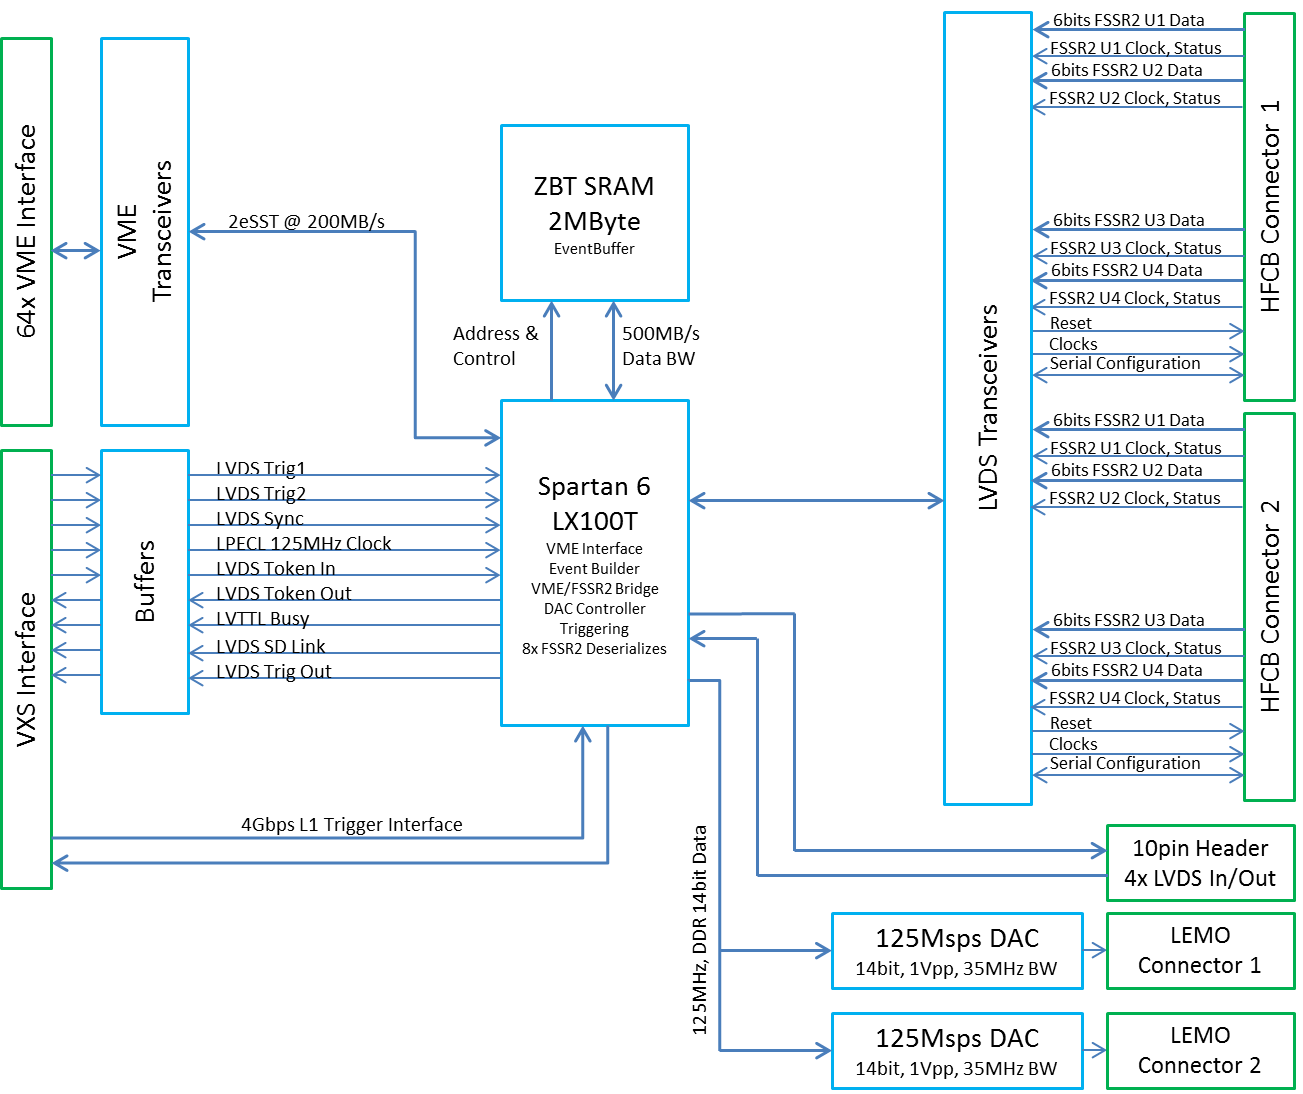
\includegraphics[width=1.0\columnwidth,keepaspectratio]{img/vscm_blockdiagram.png}
	\caption{VSCM Hardware Diagram}
	\label{fig:vscm_blockdiagram}
\end{figure}


\subsection{SSP Board as ffber Readout Module}

The SubSystem Processor (SSP \cite{ssp-ref}) was originally designed to work as part of CLAS12 Trigger System. It is used to readout some front-end electronics in the DAQ system as well. The board description can be found in the CLAS12 Trigger System article \cite{trig-ref}.
\section{High Level Synthesis in CLAS12 Trigger System Development}
\label{sec:hls}

A significant portion of the Trigger System components were developed using Vivado High-Level Synthesis (HLS) from Xilinx \cite{hls-ref}. HLS was introduced to reduce the electronics knowledge required to design hardware. It also makes the hardware design flow easier when it comes to achieving a certain behavioral model required by the hardware without worrying too much about the electronics underneath.

\subsection{Motivation to use HLS}

HLS makes it easier to incorporate well-established data processing algorithms, typically written in C++ or other high-level languages, into FPGA-based projects. HLS allows for scientists to be involved in the CLAS12 Trigger System development who do not have an electronics engineering background. It allows for the involvement of programmers who developed the algorithms for offline data processing but who have limited or no FPGA programming experience. It also makes it possible to validate code with the offline processing framework.

\subsection{Trigger Components Implemented with HLS}

HLS was used to develop most of the Stage 1 components of the CLAS12 trigger. These include the following elements:

\begin{itemize}
	\item High Threshold Cherenkov Counter (cluster energy reconstruction);
	\item Forward and Central Time-of-Flight Counters (clustering and timing correction);
	\item Electromagnetic and Preshower Calorimeters (cluster energy and position reconstruction).
\end{itemize}

The Time-of-Flight System and Cherenkov counter trigger implementation was rather straightforward. This typically takes less than 10-15\% of the Virtex-7 chip and the timing requirements were easily met.

The calorimeter trigger implementation required much more effort because of its complex nature that requires significant FPGA resources. The details are further explained in the next section using the ECAL as an example.

It should be mentioned that it took a significant amount of time to implement the desired ECAL algorithm, mostly because of the lack of experience in HLS usage. As soon as all important details of the HLS tool were understood, the development process converged, and the trigger components related to various other CLAS12 detectors were implemented in a prompt manner.


\subsection{CLAS12 Electromagnetic Calorimeters (ECAL)}

Among all of the Trigger System elements, the most challenging for the FPGA implementation was the trigger component serving the two CLAS12 electromagnetic calorimeters. Due to their structure, these calorimeters do not provide cluster coordinates or energies without significant event reconstruction. The trigger implementation details are described in Section \ref{sec:ECAL}. Below we describe our experience with HLS using ECAL as an example.


\subsection{C++ vs. HLS C++}

The FPGA implementation of the ECAL trigger was done in a 125~MHz domain, a balance between speed and resource utilization. The Trigger System components, in general, require a fixed latency, which sets certain constraints on the design. The reconstruction algorithm borrowed from the offline analysis framework was adopted for VIVADO HLS by rewriting it to C++, using HLS streams, HLS pragmas, unrolling for-loops, pipelining, and making all other needed changes. The resulting implementation was tested on simulated data and showed correct results. After that we started to run it through VIVADO HLS and VIVADO tools to address various issues related to generating an FPGA image that met the timing requirements and fit within the resource allotment.


\subsection{HLS and HDL}

When HLS is used, compiling the design consists of the following main steps:

\begin{itemize}
	\item VIVADO HLS - convert C++ to Hardware Description Language (HDL);
	\item VIVADO synthesis - HDL to FPGA primitives;
	\item VIVADO implementation - map FPGA primitives to chip and route connections.
\end{itemize}

For large designs, VIVADO HLS will very often report extremely optimistic results that suggest a viable solution, but during VIVADO implementation will fail to meet the timing requirements. To address this the failing paths must be traced back to the HLS component where it can be changed to try to improve the design. It often took many iterations to either find the workable HLS settings, code structure, or clock period adjustment.

\subsection{HLS Clock Domain}

For the different trigger components related to the different CLAS12 detectors, we use different clock domains between 250~MHz and 31.25~MHz. In the 250~MHz domain, the modules occupying more than 10\% of a XC7V550 Xilinx FPGA failed to meet the timing requirements. In the 125~MHz and lower frequency domains, the FPGA utilization was close to 100\%. For the ECAL project with a chip utilization of about 70\%, the 125~MHz clock was used.

In general, a slower clock speed (31.25~MHz) was preferable for smaller projects where resources were plentiful. When using a slow clock, the HLS code was able to be written as a single module and had no problem meeting the timing requirements during implementation.

Larger projects, such as for the ECAL, require more efficient use of the FPGA resources and have latency requirements that require a faster clock, but cannot be too fast such that the HLS modules cannot reliably meet the timing requirements. The 125~MHz clock was found to be the optimal middle ground for the ``-1'' speed grade Virtex-7 used in the CLAS12 Trigger System.


\subsection{HLS Project Size and Organization}

The typical HLS project for the CLAS12 Trigger System contains only a few routines, and uses HLS streams in the function parameter list to communicate easily with the surrounding HDL. That scheme works well for small projects.

For the ECAL with some versions being close to 100\% of FPGA utilization, the situation was quite different.
The biggest problem we faced was the inability to meet the timing requirements during the implementation (even when HLS reports that the timing is good). HLS uses state machines to schedule the operations it synthesizes. For large HLS components, the generated state machines can have massive control signal fanouts. As the clock period shrinks, so must the maximum signal fanout for the general control signals for a design to reliably meet the timing requirements. For a clock period of 8~ns using a ``-1'' speed grade Virtex-7, each HLS module was kept smaller than the 30k look-up tables (LUTs) ($<$10\% of the LUT resources) to achieve a design that consistently meets the timing requirements.

The original ECAL project consisted of about 20 C++ procedures that occupied most of the FPGA resources - with HLS generating big fanouts on this scale, it was impossible to meet the 8~ns timing on the implementation stage. The workaround was to split the entire project into smaller procedures, glued together in HDL by using well defined, simple interfaces between the separate procedures. Still, some procedures were too big, especially for the sorting algorithms. We were able to split some procedures further until finally the entire project met the timing requirements and the resulting FPGA image was loaded into the hardware.

After every significant change, we re-tested the code on simulated data, making sure it still produced correct results. The chart in Fig. ~\ref{fig:hls_chart} shows how many HLS projects were created in the end.

Another reason for subdividing the project is the lack of multi-clock domain support. Since the Event Builder in the VTP board works on a 250~MHz domain and most projects use a slower clock, every project was subdivided and separate pieces communicated over the HDL-written interface. The necessity of subdividing HLS projects and of using HDL to assemble them together, is probably the most restricting feature in HLS usage. Much of this subdividing can be reduced by using the HLS DATAFLOW directives (which can isolate functions communicating through registered FIFO interfaces), but it requires further code restructuring to be compatible with this flow and does not support multiple clock domains.

\begin{figure}[hbt]
	\centering
	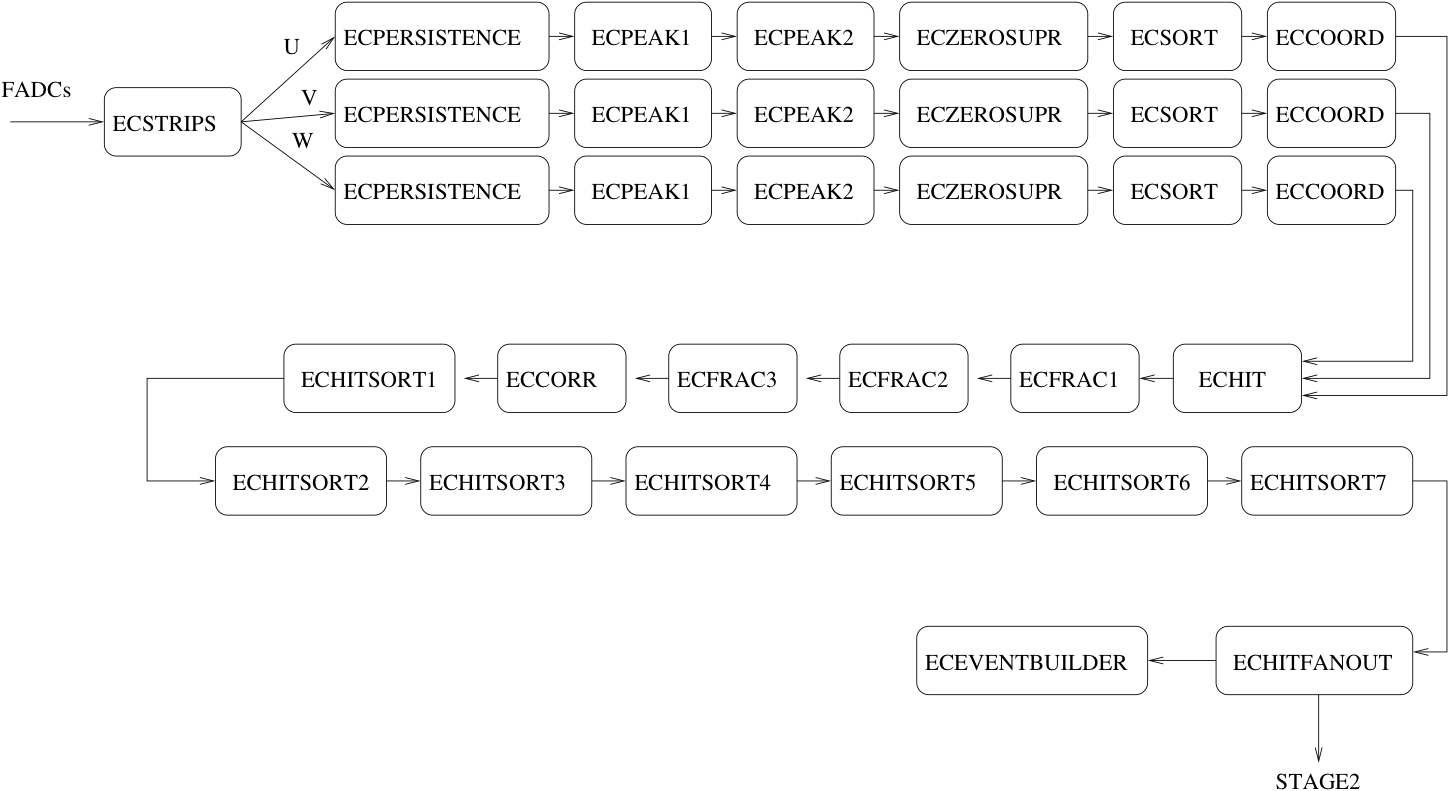
\includegraphics[width=1.0\columnwidth,keepaspectratio]{img/hls_chart.png}
	\caption{ECAL HLS project chart. The entire project is split into multiple smaller projects to satisfy the timing requirements. In particular, the hit sorting section is split into seven identical projects.}
	\label{fig:hls_chart}
\end{figure}


\subsection{HLS Versions and Cross-Project Dependences}

As mentioned before, splitting the project into smaller pieces allowed us to meet the timing requirements. This worked, in particular, because we were able to eliminate combinatorial paths between the HLS projects connected by the streams. Such dependences can be clearly seen looking into the schematics for the failed timing chains, and were usually related to the large state machine control signals going between modules. Initially we used HLS version 2015, and despite all of our efforts, we could not eliminate these long combinatorial paths across modules. This was resolved after switching to HLS version 2017, where the streams could be fully registered (with pragma ``axis register both port=''). This meant that if the registered HLS streams were used between separate HLS projects, then the state machine paths were also registered between modules. With that, it was only a matter of splitting projects into smaller pieces to improve/meet the timing requirements.


\subsection{HLS Settings}

The clock uncertainty is set as 30\% of the main clock, which we found forces HLS to produce more realistic timing estimates. A single HLS project often cannot exceed several percent of the flip-flops (FF) and LUT budget, otherwise it may be a problem to meet the timing requirement on the VIVADO implementation step. A typical HLS project for one of the PCAL trigger elements is shown in Fig. ~\ref{fig:hls}.

\begin{figure}[hbt]
	\centering
	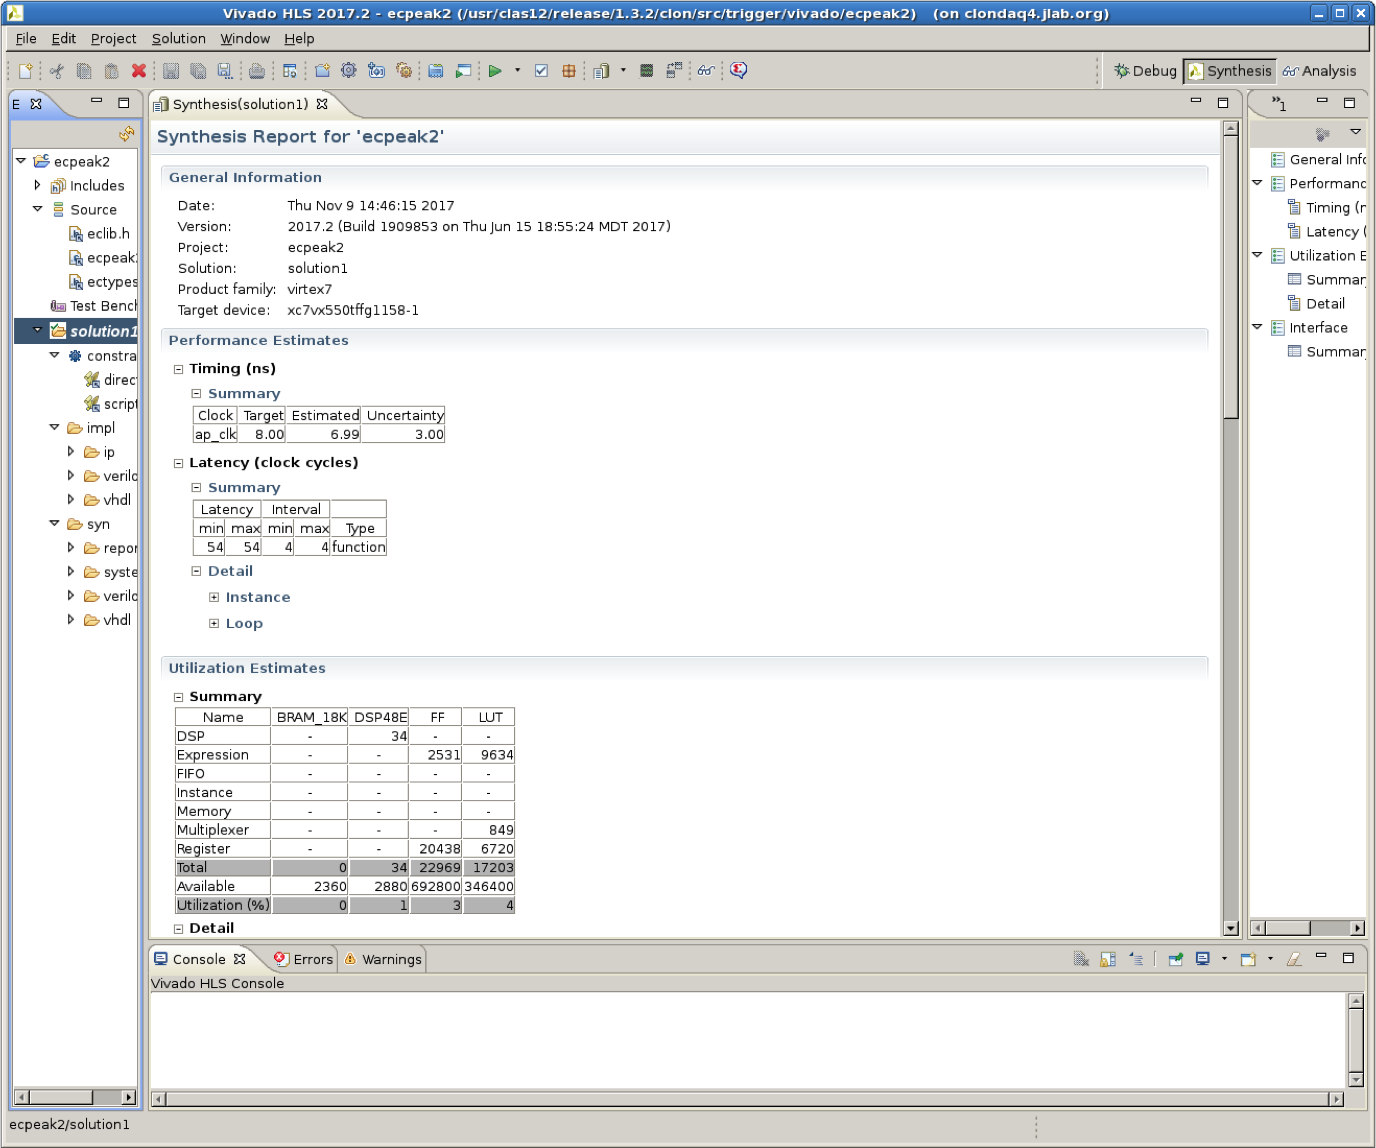
\includegraphics[width=1.0\columnwidth,keepaspectratio]{img/hls.png}
	\caption{Typical HLS project for one of the PCAL trigger elements. 4\% LUTs is close to the maximum possible to meet the timing requirements of the following steps. With an 8~ns target, the clock uncertainty  is set to 3~ns.}
	\label{fig:hls}
\end{figure}

\subsection{VIVADO Settings}

Common settings for VIVADO were used as shown in Fig. ~\ref{fig:vivado}. It usually takes 3+ hours to compile the PCAL project on a Dell R730 server under RHEL7. For some firmware versions, we were able to utilize 100\% of the LUTs and still meet the timing requirements if the clock domain was 125~MHz or lower. The VIVADO project for the PCAL trigger is shown in Fig. ~\ref{fig:vivado}.

\begin{figure}[hbt]
	\centering
	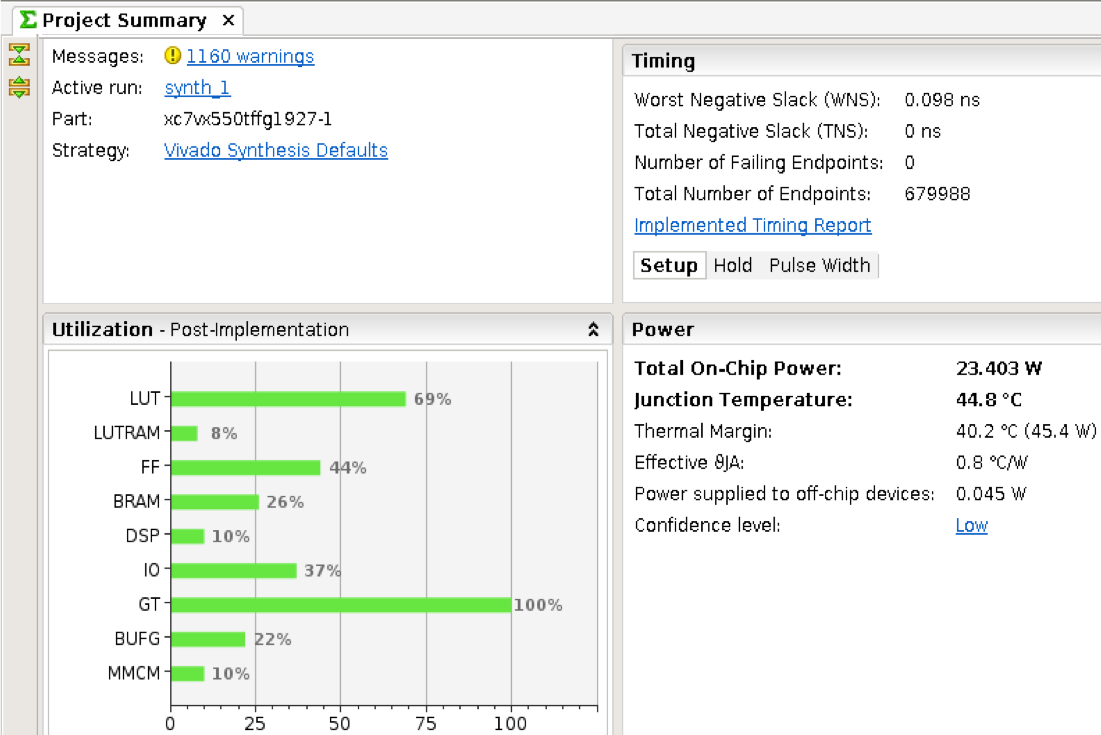
\includegraphics[width=1.0\columnwidth,keepaspectratio]{img/vivado.png}
	\caption{VIVADO project for the PCAL trigger. Strategies used were ``Vivado Synthesis Defaults'' and ``Performance\_ExplorePostRoutePhysOpt''. LUT utilization is about 2/3 of the total balance. It was relatively easy to meet the timing requirements with an FPGA clock 125~MHz or slower.}
	\label{fig:vivado}
\end{figure}

\subsection{Firmware Validation for HLS-based Projects}

The ability to validate the firmware using a C++ implementation is the one of the biggest advantages of HLS. During the course of development and commissioning, we ran HLS C++ code on simulated and real data from the CLAS12 detectors, implementing required features and fixing bugs. During data taking we were able to find and fix observed problems or add new features in several hours, which was very important to save beam time.

\subsection{Our Conclusion about HLS Usage}

The CLAS12 ECAL and other detectors were successfully implemented into the Trigger System using HLS to produce the core part of the firmware. This trigger was used in the first physics run in 2018 and worked as expected. We were able to select events based on individual ECAL cluster energy, something which was possible before only during offline data processing.

HLS in general appears to be a useful tool, especially to implement smaller trigger components like the Cherenkov or Time-of-Flight counters. For components utilizing a significant portion of the FPGA, it will benefit development significantly to improve HLS in the following directions:

\begin{itemize}
	\item Support multi-clock domains;
	\item Improve subroutine calls by allowing the option to fully register paths between modules; 
	\item Improve state machine logic, for example support streams between routines inside the project and be able to generate separate state machines for separate routines. This will allow for the avoidance of splitting the project manually and using HDL as a top interface as we are currently forced to do.
\end{itemize}

\section{Software}

\subsection{... CODA DAQ software ... (Abbott)}

CLAS12 DAQ system is based on CODA (Fig.~\ref{fig:coda_diagram}), short for CEBAF Online Data Acquisition. It is a kit of parts that allows the researcher to implement a data acquisition system. The scale of the system can range from a few detector channels in a test stand to tens of thousands of channels in a large detector installation in one of the halls. CODA achieves this scaling through modularity and provides a set of hardware components along with complementary software components.

\begin{figure}[hbt]
	\centering
	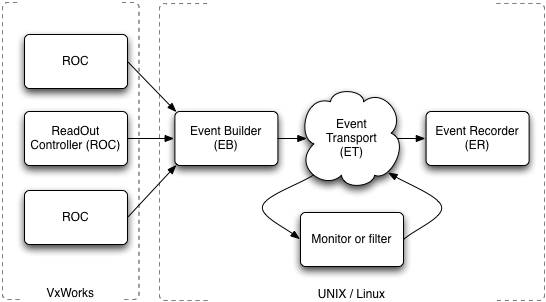
\includegraphics[width=1.0\columnwidth,keepaspectratio]{img/coda_diagram.png}
	\caption{CODA System Diagram}
	\label{fig:coda_diagram}
\end{figure}


\subsection {Runcontrol(Sergey)}

The CODA DAQ system includes a run control facility consisting of a back-end run control supervisor and a front-end graphical operator display that connects to the supervisor and controls its operation. The supervisor in turn controls operation of the many CODA components that participate in the run. The latter are defined in run configuration files that the operator chooses at startup. The gui presents the operator with a choice of possible actions that depend on the current state of the run. The supervisor translates the operator choice into appropriate commands to the individual components. Alternatively, limited communication with the supervisor can be performed via command-line scripts.
The supervisor in addition monitors the health and operation of the CODA components and warns the operator or pauses the run if problems are detected.


\subsection{Front End Libraries(Moffit)}

\subsection{Frontend Libraries}

Just an outline ATM

GEFANUC driver:
\begin{itemize}
\item Customized Kernel Driver and Userspace Interface
\item C API provides:
   \begin{itemize}
   \item Setup of VME inbound and outbound windows
      \begin{itemize}
      \item Permanent windows: CRCSR, A16, A24, A32
      \item Map of these windows into userspace
      \end{itemize}
   \item Allocate of Physical Memory for DMA
      \begin{itemize}
      \item Map of this memory into userspace
      \end{itemize}
   \end{itemize}
\end{itemize}

JVME Userspace Driver:
\begin{itemize}
\item C API provides
  \begin{itemize}
  \item common userspace interface to GEFANUC driver and others.
  \item Initialization of kernel driver and default VME windows
  \item Maps VME bridge registers into userspace
    \begin{itemize}
    \item Provides userspace configuration and operation of DMA
    \end{itemize}
  \item Initialization of and access to shared memory mutex for intra-process cooperation during DMA
  \end{itemize}
\end{itemize}

Frontend Libraries
\begin{itemize}
\item C APIs provide
  \begin{itemize}
  \item module register mapping in VME windows to memory structures.
  \item configures modules for readout via
    \begin{itemize}
    \item programmed i/o
    \item Single module DMA
    \item Multiple module DMA
       \begin{itemize}
       \item Token passing (P0/VXS and CBLT) with common A32 address range
       \item Linked List DMA
       \end{itemize}
    \end{itemize}
  \end{itemize}
\end{itemize}



\subsection{Readout Controller(Abbott)}

Readout Controller (ROC, Fig.~\ref{fig:roc_diagram}) software component is the program running on front-end controllers such as Intel-based VME/VXS crate controllers, VTP trigger boards or regular Linux servers - any hardware receiving data from front-end electronics. On the DAQ startup ROC main program starts three threads, after that it just controlls thread health and communicates with run control process. Three threads (readout, processing and network) are passing data from one to another communicating over circular buffers. Typical number of buffers in each circle is 8 and size of every buffer is 4 MBytes, which defines how long front-end electronics will be read out before feeling effect of the back-end busy conditions.

First (readout) thread receives data from front-end electronics and places them into first circular buffer. That thread can run in pooling mode occupying entire cpu core, or in interrupt mode. CLAS12 are using mostly pooling mode which has adequate performance on multi-core controllers.

Second (processing) thread reads data from first circular buffer and perform needed data processing, in particular it does so-called disentangling and data sanity check. Results placed into second circular buffer. That component can create its own threads to burst processing power.

Third (network) thread reads data from second circular buffer and send it over network to the Event Builder.

First and second threads have user part which compiled separately and downloaded dynamically, it allows users to develop experiment-dependent code without recompiling CODA framework.

\begin{figure}[hbt]
	\centering
	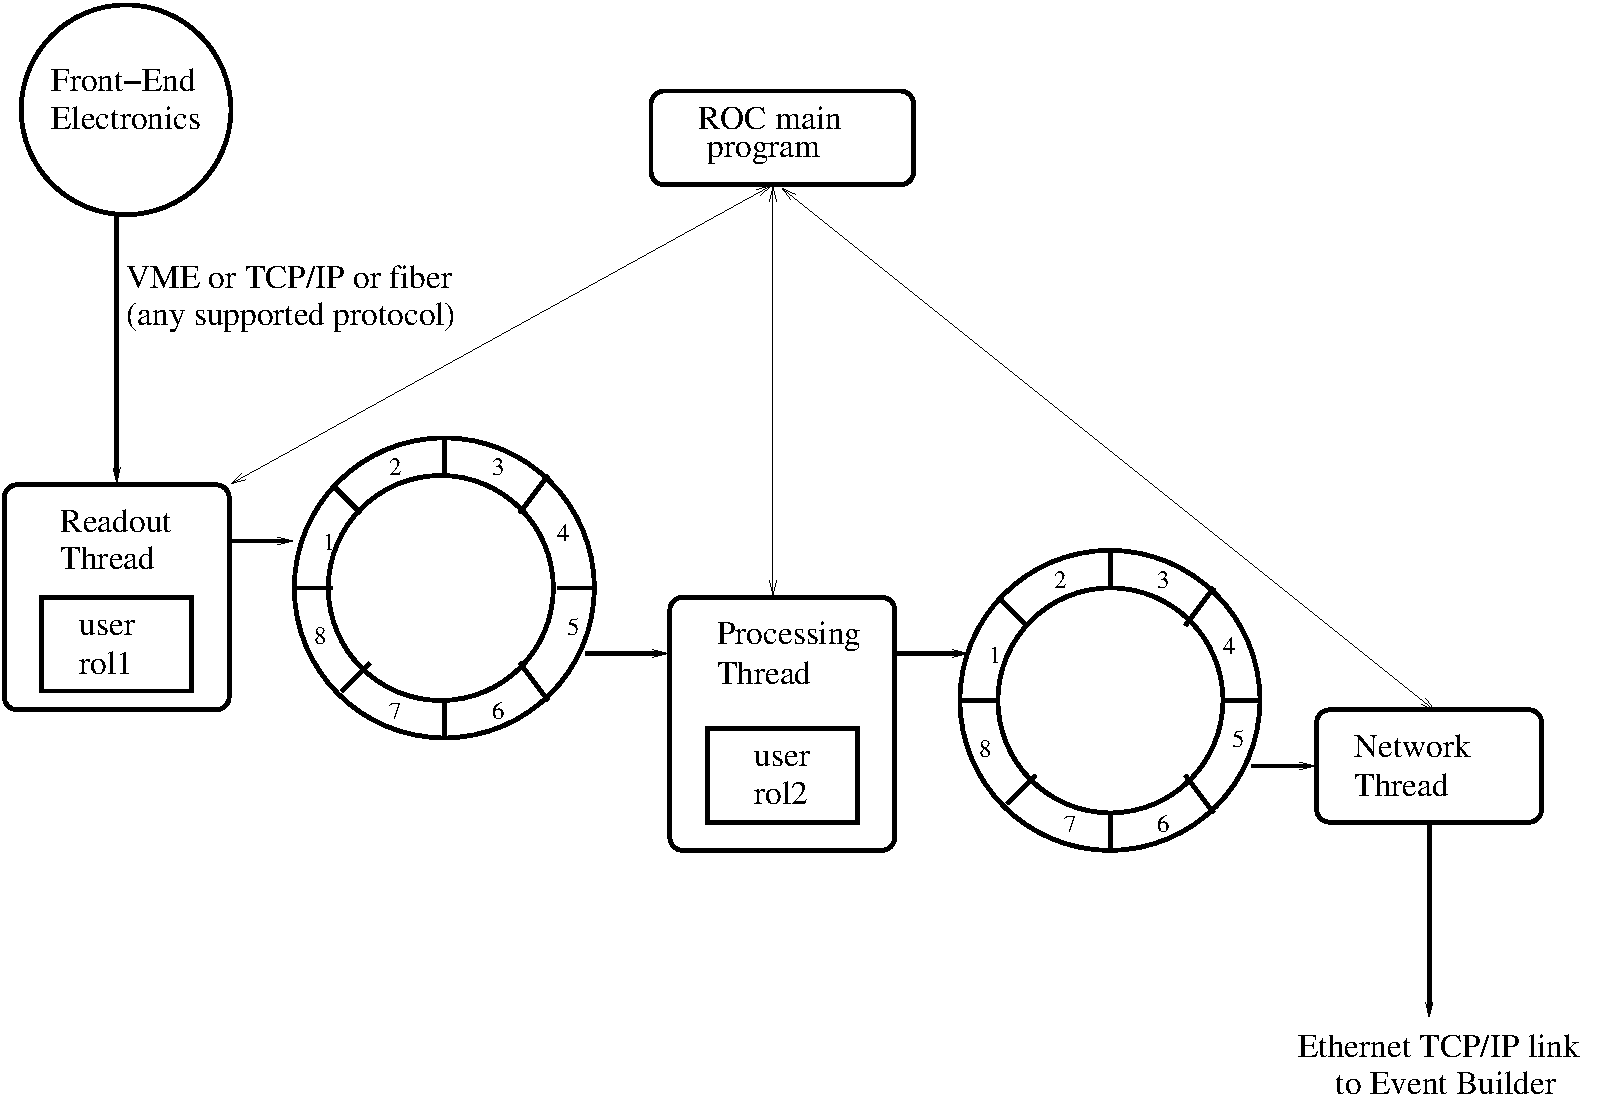
\includegraphics[width=1.0\columnwidth,keepaspectratio]{img/roc_diagram.pdf}
	\caption{Readout Controller Diagram}
	\label{fig:roc_diagram}
\end{figure}


\subsection{Event Builder (Graham)}

Event Builder (EB, Fig.~\ref{fig:eb_diagram}) is the program receiving data fragments from all readout controllers and glueing it into events. Building process is based on event number, event type and timestamp of the data fragments: for every particular event all three values have to be identical for all data from all readout controllers. In case of any difference DAQ will be stopped and error reported.

Event Builder consists of receiving and building parts. Receiving part contains set of independent threads, one per readout controller connected to it by TCP protocol. Every thread receives data and place it into internal buffer. If buffer becomes full thread stops receiving data, effectively propagating busy condition back to readout controller.
Building part has the number of identical building threads, which takes turns by getting data from receiving part internal buffers, building events and placing them into Event Transfer System.

Total number of Event Builder threads in CLAS12 DAQ is currently 118, so the number of network connections from readout controllers. Because of that it have to run on powerful server, usually the one with many cpu cores, big memory and high bandwidth network card. CLAS12 is using DELL R730 server with 32 cores, 64GByte memory and 40Gbit network card. That server is adequate for CLAS12 DAQ requirements.

\begin{figure}[hbt]
	\centering
	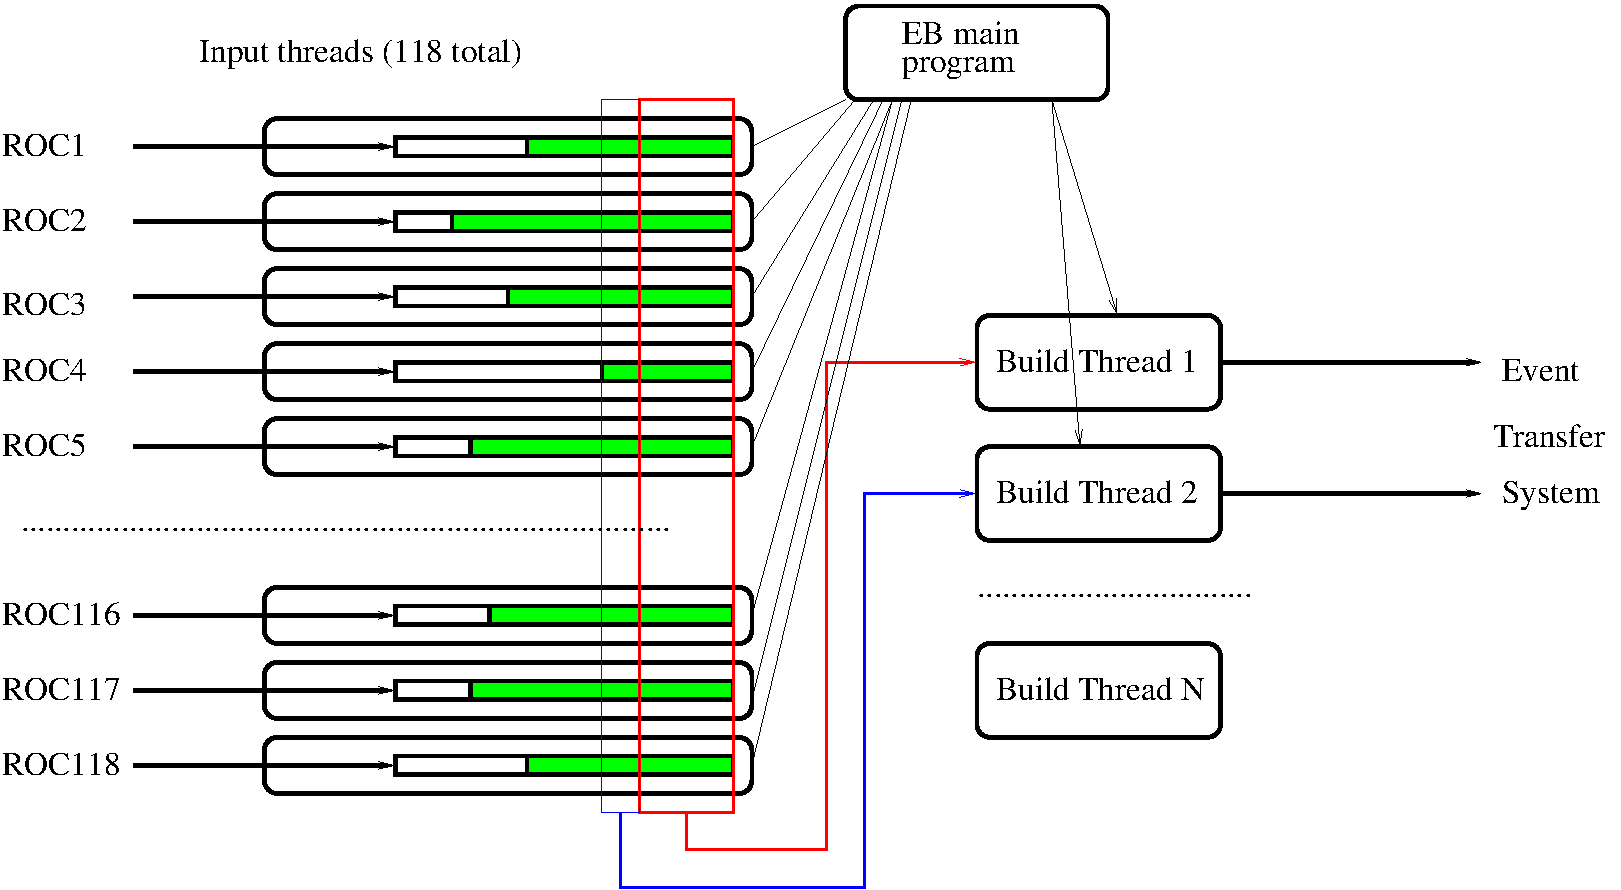
\includegraphics[width=1.0\columnwidth,keepaspectratio]{img/eb_diagram.pdf}
	\caption{Event Builder Diagram}
	\label{fig:eb_diagram}
\end{figure}


\subsection{Event Transfer (Carl)}

Event Transfer (ET) system allows multiple connections to the data stream, needed for online data monitoring and possibly data or/and event reduction. It consists of ring of buffers, one per event, filled by Event Builder and accessed by one or several processing programs. Every processing program can request to see every event or subset of events based on selecting algorithm. There is a possibility to access ET system remotely, as well as create a chain of ET systems running on different servers effectively increasing processing power. Last program attached to ET system usually Event Recorder.

\subsection{Event Recorder (Sergey)}

Event Recorder (ER) is the program receiving data from ET system and recording data files into the disk. It can write data in one or several files in parallel (so-called multi-stream mode). If multi-stream mode is used event order is preserved, but it requires the allocated memory size to be bigger then the number of streams multiplied by the file size.


\subsection{Messaging System (ActiveMQ) (Sergey)}

Messaging system in CLAS12 DAQ is based on ActiveMQ library and its C++ extension. Two ActiveMQ servers used to route all communiations. The number of connections to ActiveMQ is several hundreds, and the number of messages sent every second is several tens of thousands, with data volume few tens of Megabytes per second. Messaging system is used in particular to monitor and control DAQ components, in addition to the Runcontrol.


\subsection{Runtime Database (RCDB) (Sergey)}

JLAB-designed mysql-based Runtime Database (RCDB) is used to store run parameters and statistic. It has web interface (Fig.) and provides interface to various languages including C++ and Java.


\subsection{Online Data Monitoring (Raffaella,Cole)}

CLAS12 Online data monitoring is the set of programs attached to Event Transfer System and processing data in real time. One of such program's output is shown on Fig.



\subsection{CSS for DAQ, communication with DAQ (Nathan)}



\subsection{ROOT for DAQ (FT) (Andrea)}

A ROOT-based system was developed to display integrated quantities from the CLAS Trigger system in the form of 1D
and 2D histograms. The system is made by three different applications: a histogram sender running on each VTP, a
histogram receiver running on a DAQ server, and a user-configurable GUI client. Each histogram sender application
defines a set of 1D and 2D histograms to report trigger data specific to the CLAS12 subsystem handled by the VTP it is
running on. Histograms are refreshed at a fixed rate and streamed to the DAQ server in the form of JavaScript Object
Notation (JSON) messages, exploiting the previously described ActiveMQ infrastructure. Each message contains: the
histogram name, the number of bins, and a data array with the number of counts in each bin. The message receiver
application is responsible for decoding these messages, and of creating ROOT histograms from them. Finally, the client
application displays ROOT histograms to the user through a customizable GUI.

The GUI is composed of a programmable number of independent frames, with different histograms in each of them.
Typically, each frame contains histograms related to the same CLAS12 subsystem. The GUI structure is specified through
a configuration file passed as a command-line option when running the client. Communication between the message
receiver/ROOT histogram produced application and the user client is handled through the ROOT TSocket mechanism.
Figure~\ref{fig:plot_andrea} shows a GUI reporting histograms from the Forward Tagger system~\cite{ft-ref}: two
2D histograms showing the distribution of electromagnetic cluster hits in the Forward Tagger Calorimeter, and two
1D histograms showing the electromagnetic cluster energy distribution. The right (left) column reports histograms for
electromagnetic clusters  with (without) a matching hit in the Forward Tagger Hodoscope.

\begin{figure}[t]
	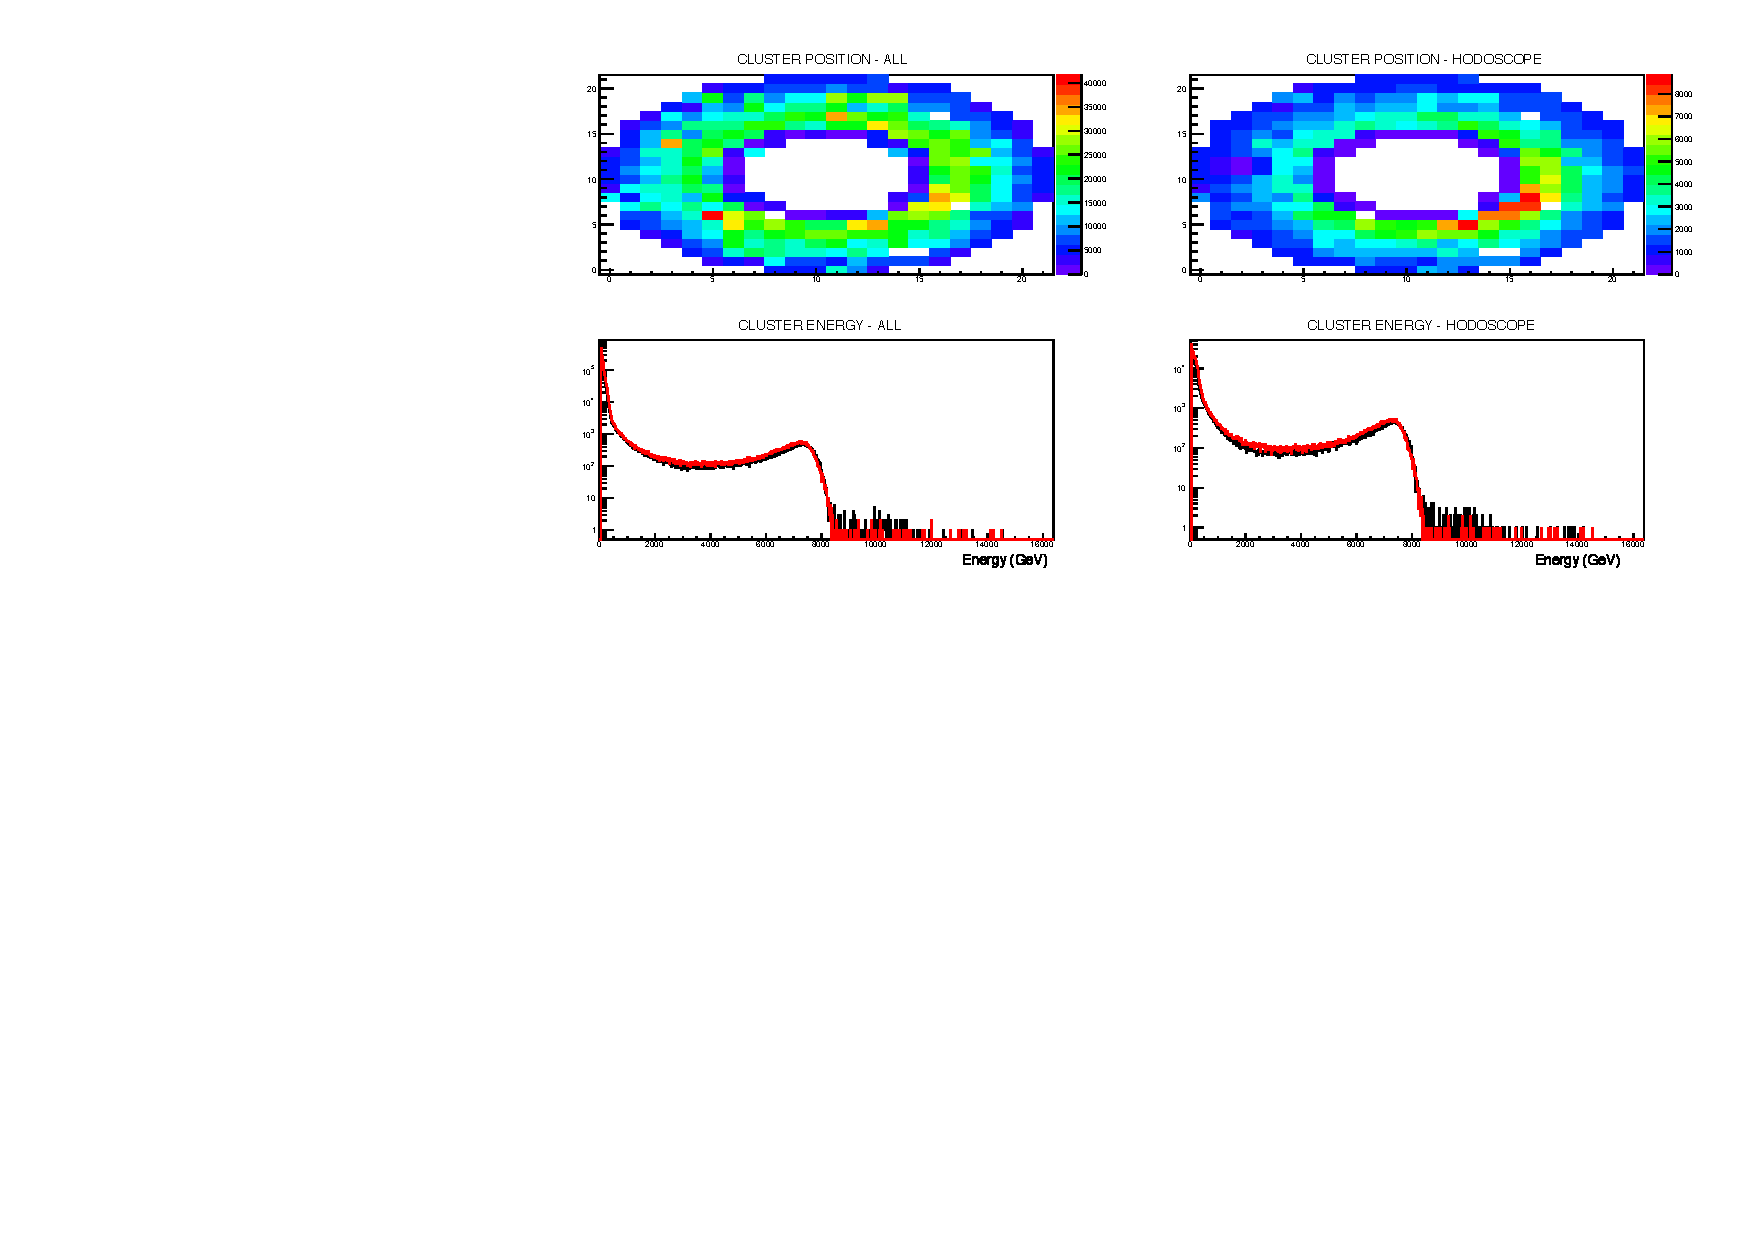
\includegraphics[width=1.0\columnwidth]{img/plotAndrea.pdf}
	\caption{Example of a ROOT-based GUI to monitor trigger data for the specific case of the Forward Tagger
        detector~\cite{ft-ref}. The top histograms report the distribution of electromagnetic cluster hit positions, while
        the bottom histograms report the electromagnetic cluster energy distribution. The right (left) column reports
        histograms for electromagnetic clusters  with (without) a matching hit in the Forward Tagger Hodoscope.}
	\label{fig:plot_andrea}
\end{figure}



\subsection{CLAS Event Display (Heddle)}

The CLAS12 event display (ced) is a full-function graphical application that displays on-line (and off-line) events using various representations of CLAS12 called views. The views are independent windows that the user can pan, zoom, scroll, etc. Some of the views are geometrically faithful, and some are designed for maximal information content as opposed to realism. The primary purpose and utility of ced, when used on-line as part of the DAQ system, is for additional monitoring. While running, ced will display an event from the live stream at a selectable rate, typically one every two seconds. A quick glance at ced will confirm, for example, that there are data in the drift chambers that appear to form tracks. In this way it serves as an early warning of problems with detectors and/or the data stream. It is also possible to operate ced in a mode where it creates graphical histograms or occupancy overlays. A typical view from ced is shown in Fig.~\ref{fig:ced}.

\begin{figure}[hbt]
	\centering
	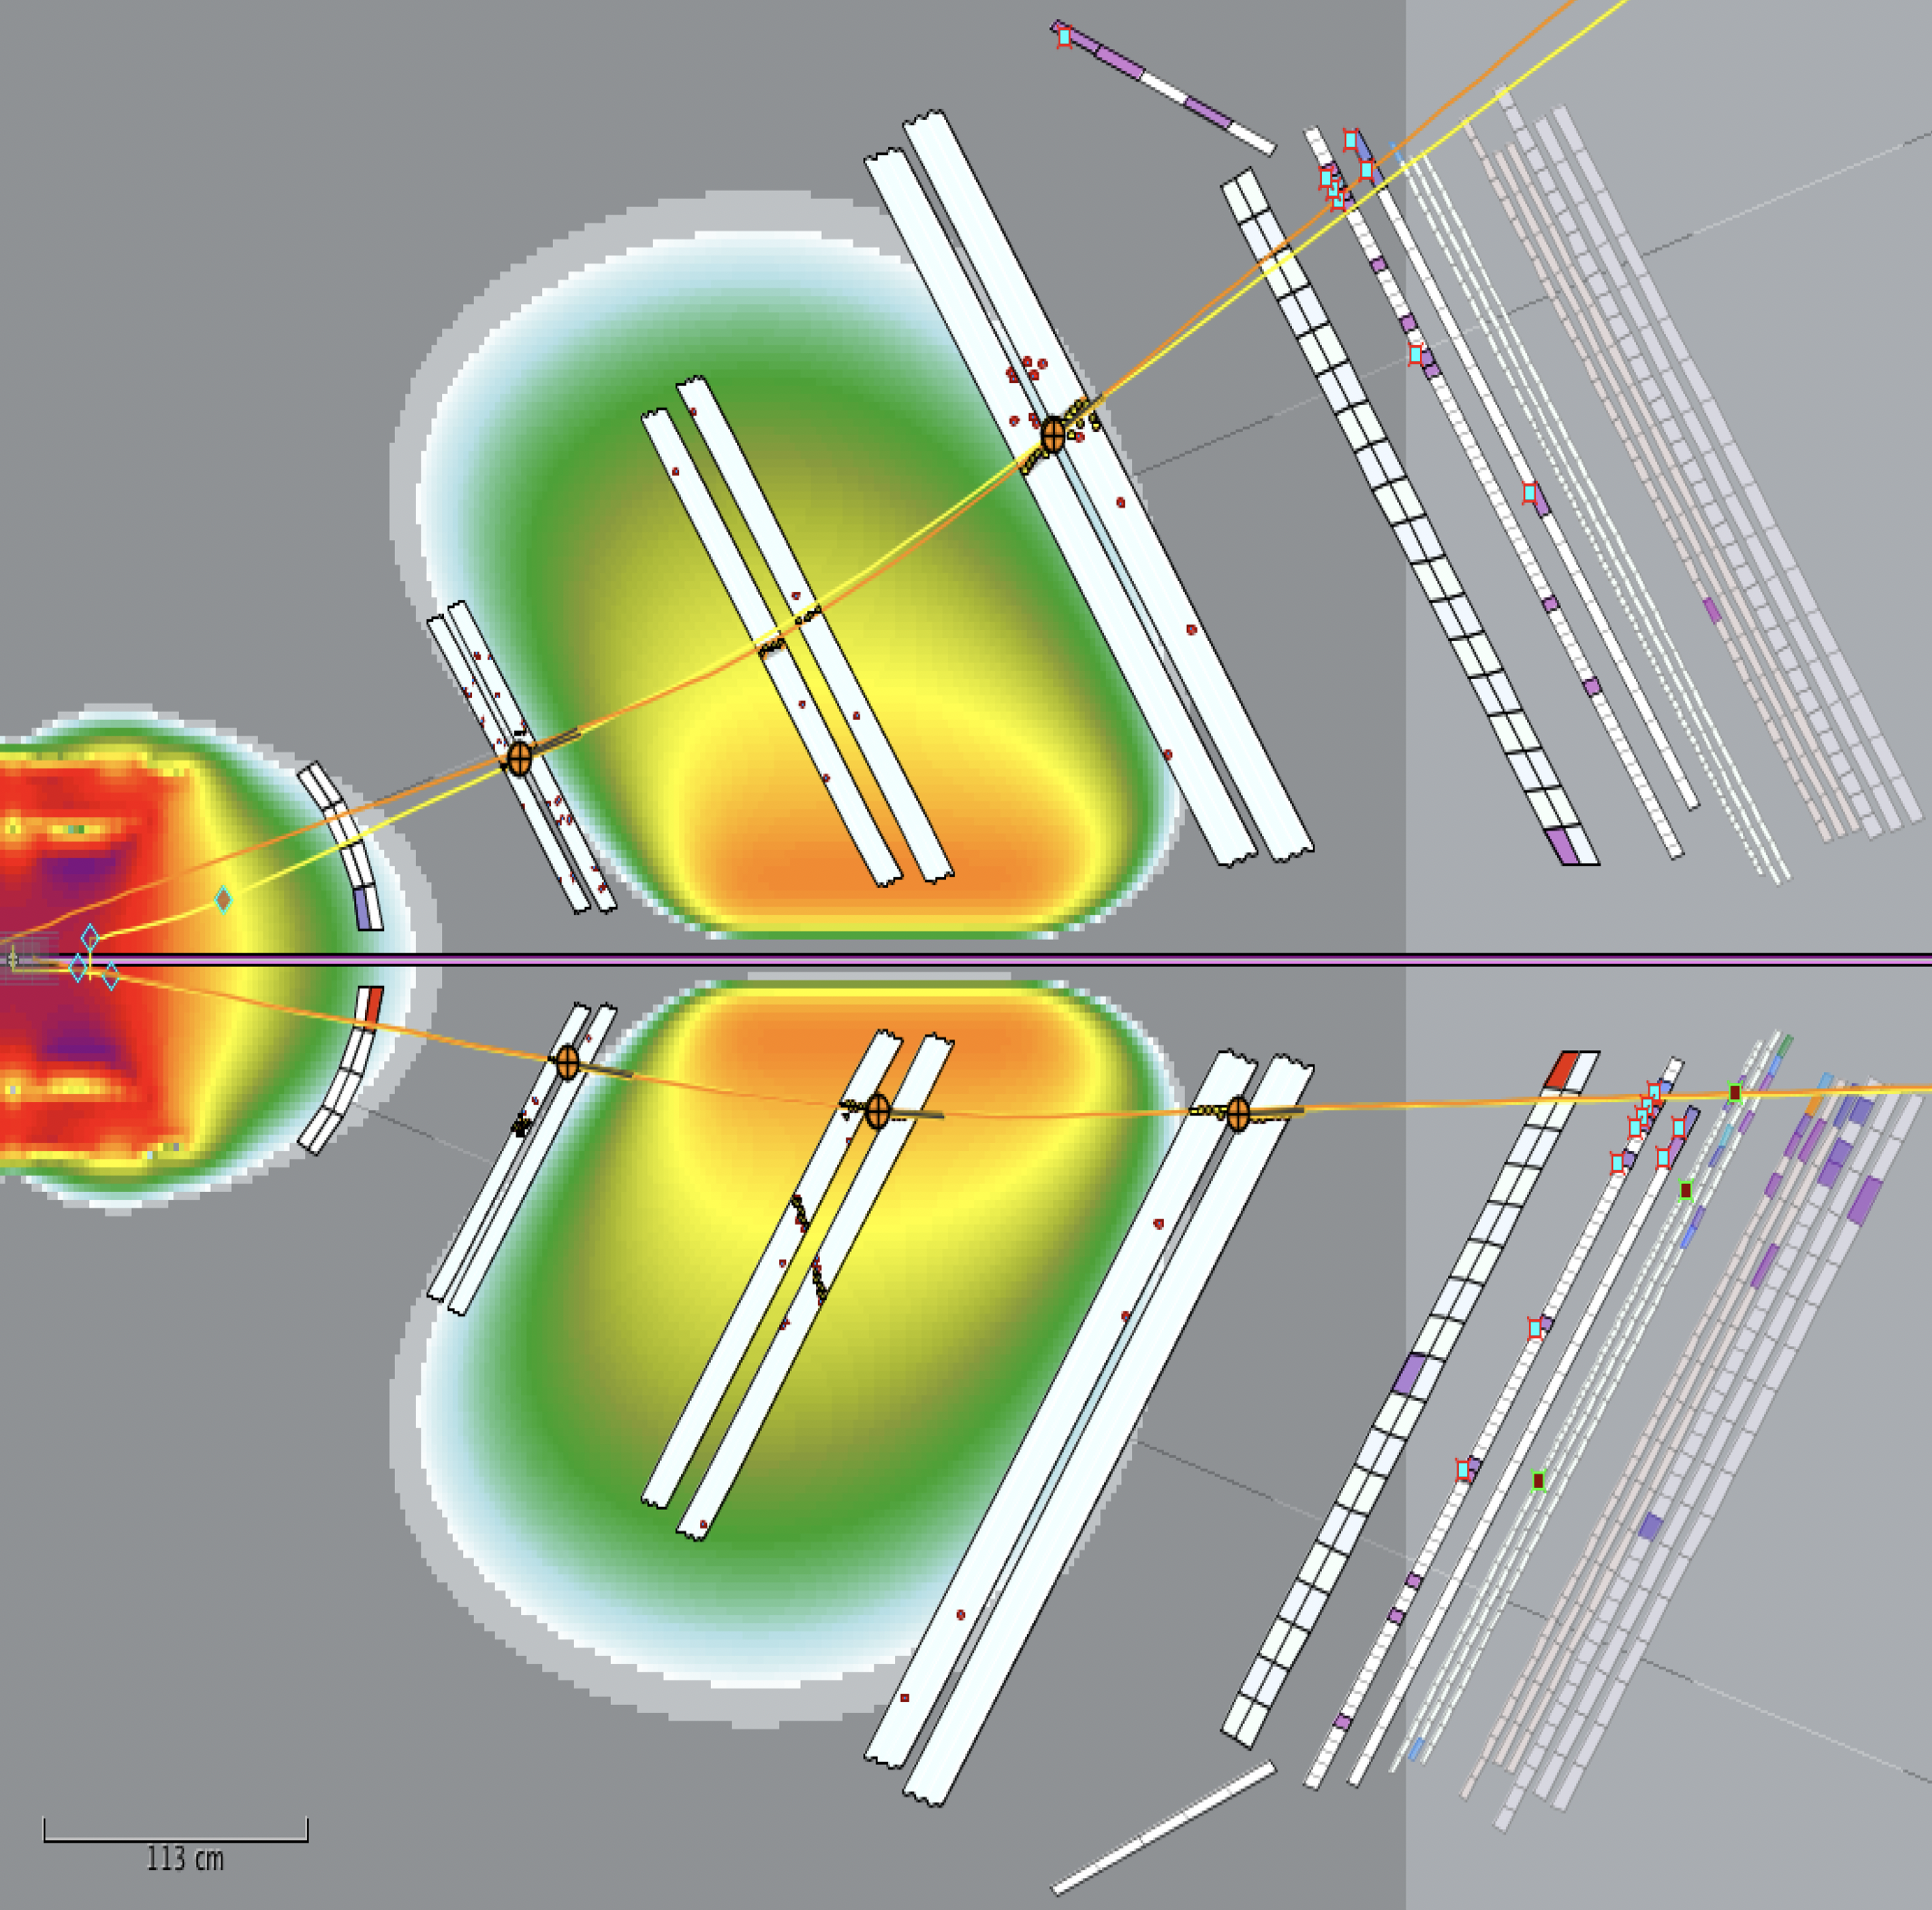
\includegraphics[width=1.0\columnwidth,keepaspectratio]{img/ced.png}
	\caption{CED Event Example}
	\label{fig:ced}
\end{figure}

\section{Simulation}

%\subsection{Expected physics performance}

%A series MC simulation have been used to calculate the acceptance of the central detector and have reconstructed physics parameters for types of events that are of interest. Fig. ... shows the missing mass resolution expected for MC simulation studies for a number of different reactions. For all cases studied, the results show that it is possible to identify the missing particle for each reaction.
%Figure ... shows the missing mass spectrum expected when pion is detected in the central tracker. There is sufficient resolution to study resonant production and to compare, for example, s, t, and u channel processes.

\subsection{Detector simulation}

A realistic model of the SVT has been developed, describing the location and composition of all modules, with material description based on the engineering drawings and assembly procedures, and confirmed by the survey measurements during integration. The SVT design and module layout were validated by Geant-4-based simulated detector performance studies demonstrating compliance with the technical requirements and engineering models. A 3D view of the simulated geometry of the SVT sensors is shown in Fig.~\ref{fig:svt3dview}. The SVT model is described in the simulation article of this volume. 

\begin{figure}[hbt] 
\centering 
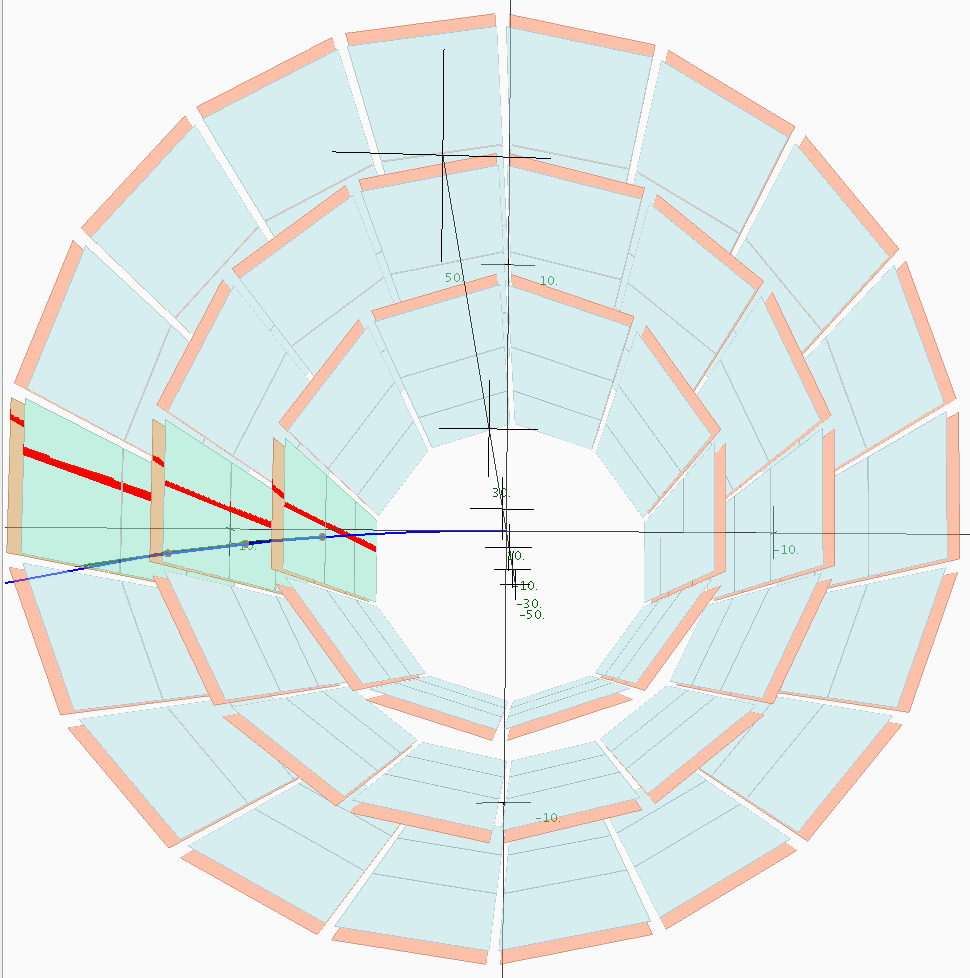
\includegraphics[width=1.0\columnwidth,keepaspectratio]{svt3dview.png}
\caption{3D view of the simulated SVT detector geometry.}
\label{fig:svt3dview}
\end{figure}

According to the results of GEANT simulation of the SVT, a resolution of 50~$\mu$m in the bending plane is needed to measure, with a precision better than 5$\%$, tracks with momentum up to 1~GeV (see Fig.~\ref{fig:PtRes}) \cite{MC1,MC2}. At low momenta the degradation of the resolution is caused by multiple scattering.

\begin{figure}[hbt]
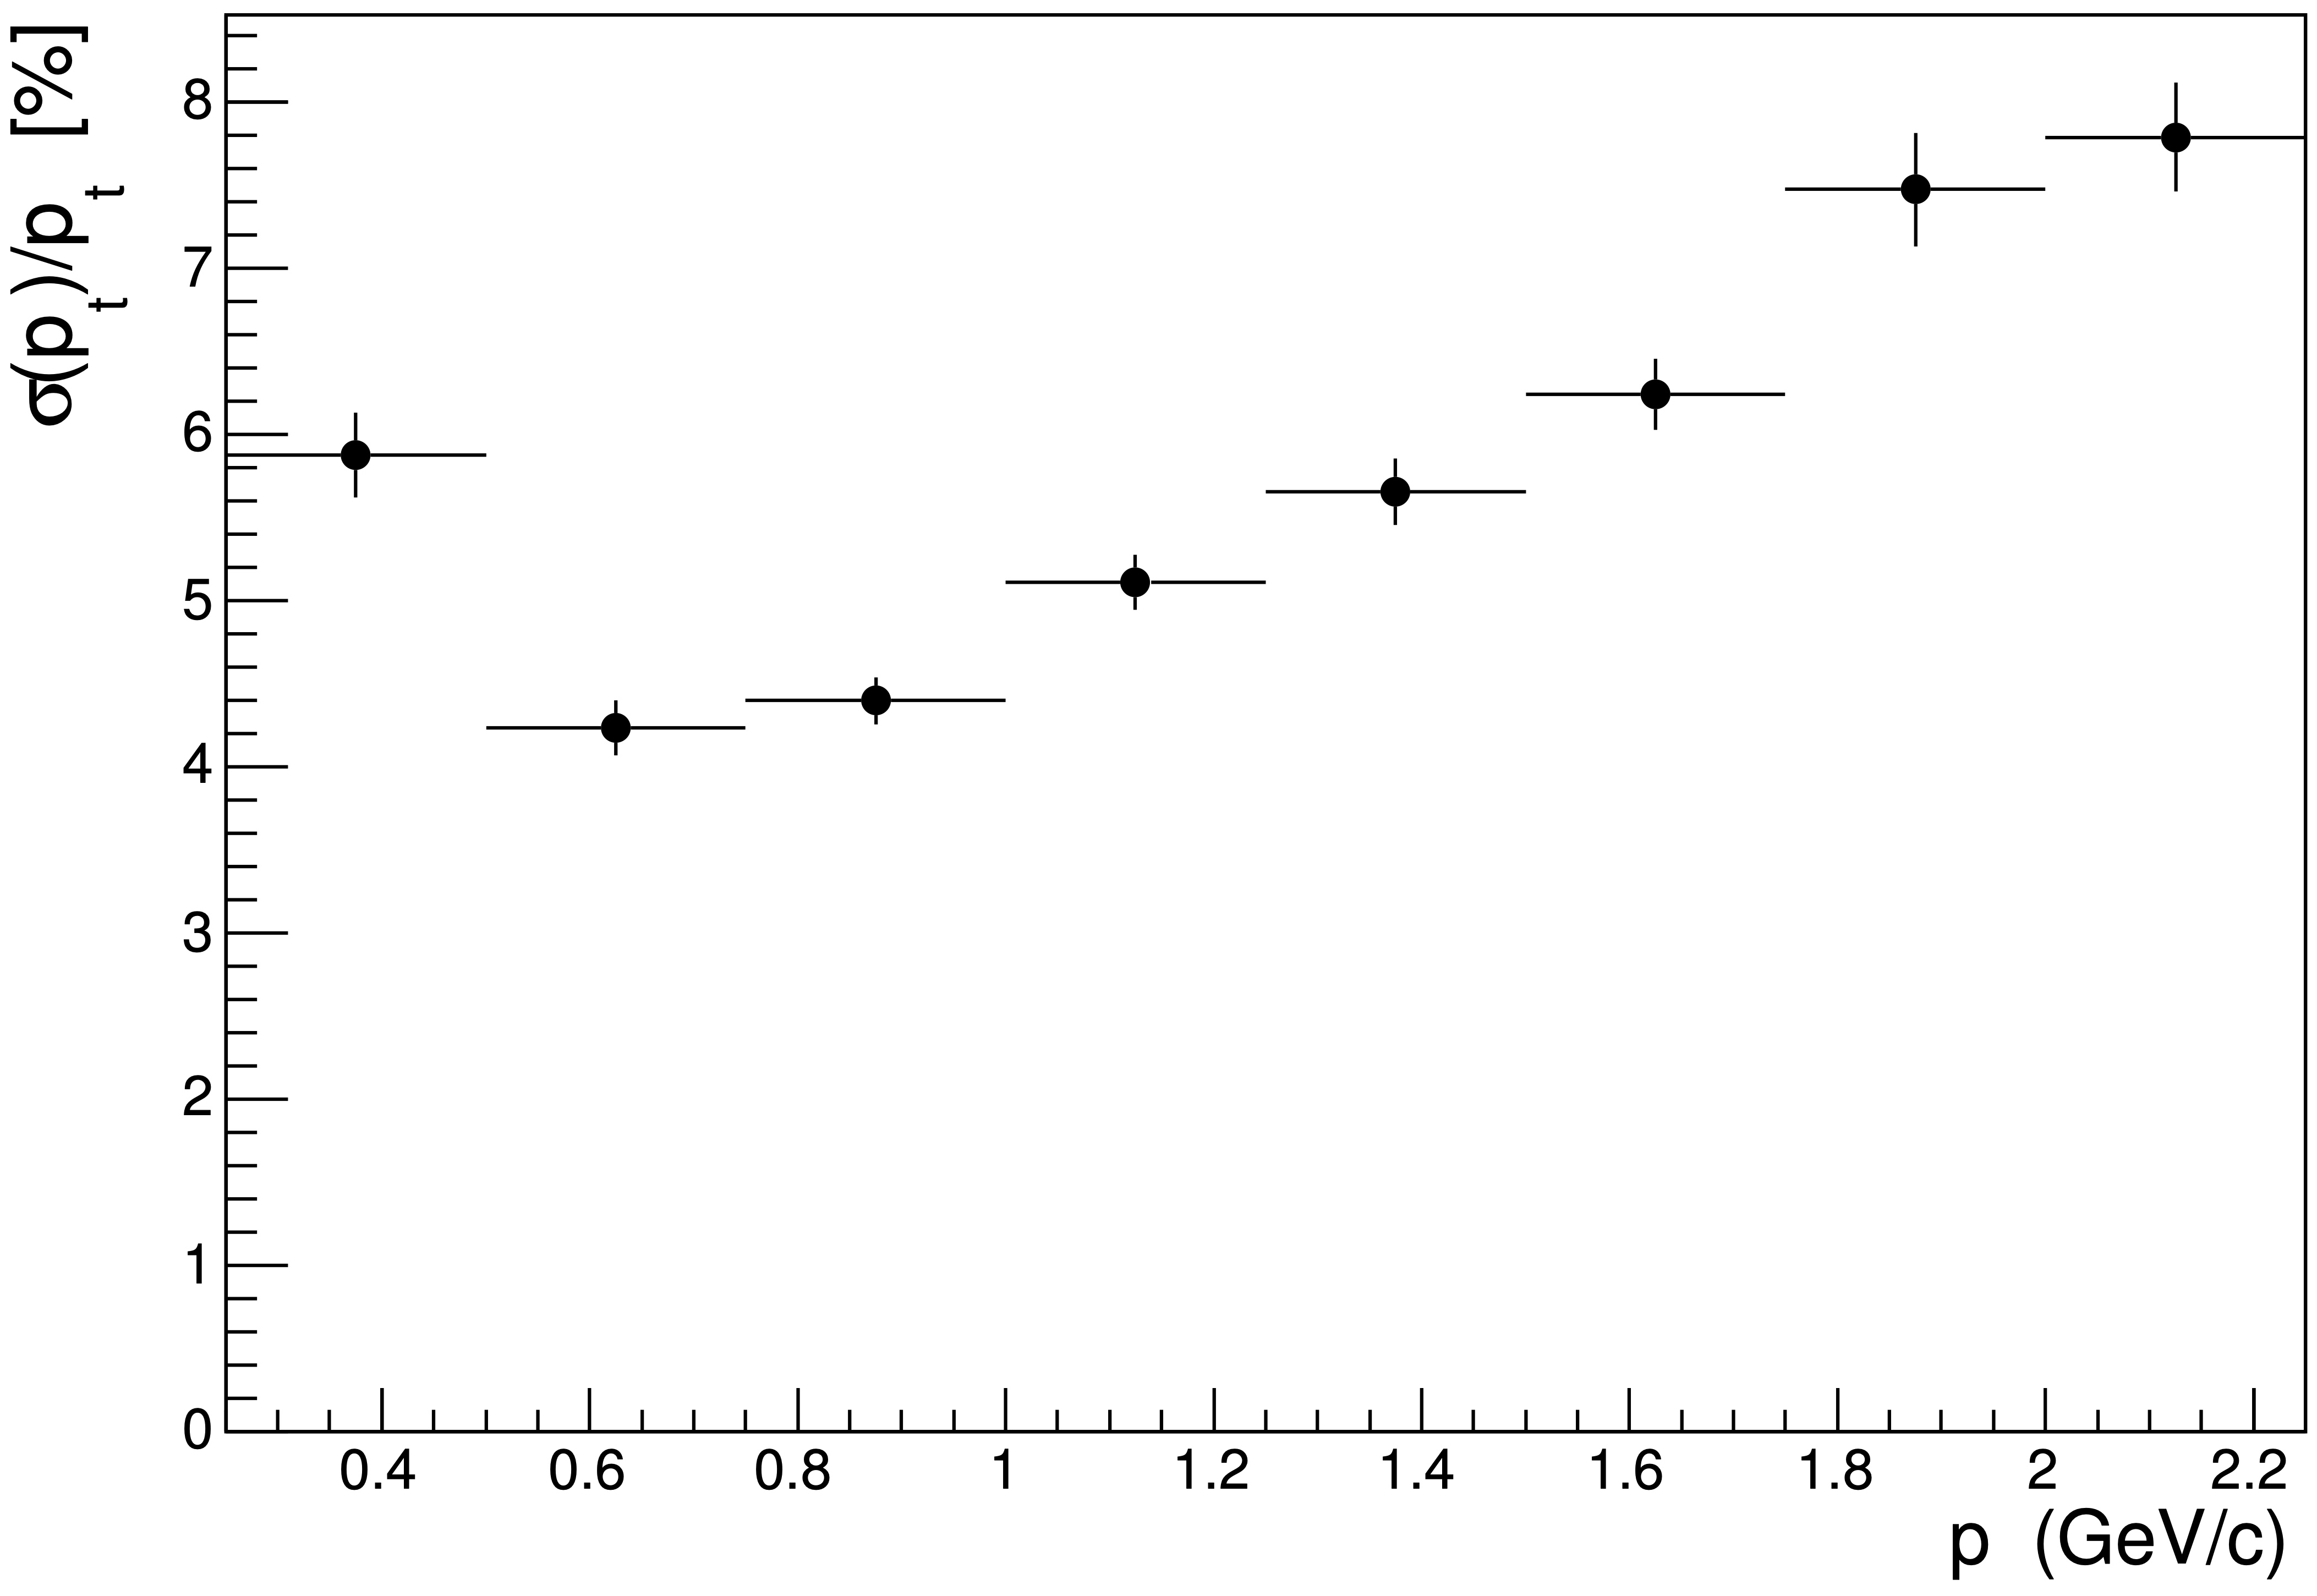
\includegraphics[width=1.0\columnwidth,keepaspectratio]{PtResol.jpg}
\caption{Simulated SVT momentum resolution.}
\label{fig:PtRes}
\end{figure}

Centroid residual distribution for the simulated muon tracks generated in the interval 0.5--2 GeV is shown in Fig.~\ref{fig:centroid-residual-mc}. Cluster centroids were calculated based on the charge weighting method. The spacial resolution of the sensors in the transverse plane using the ideal SVT geometry with no misalignments was found to be about 30~$\mu$m. 

\begin{figure}[hbt]
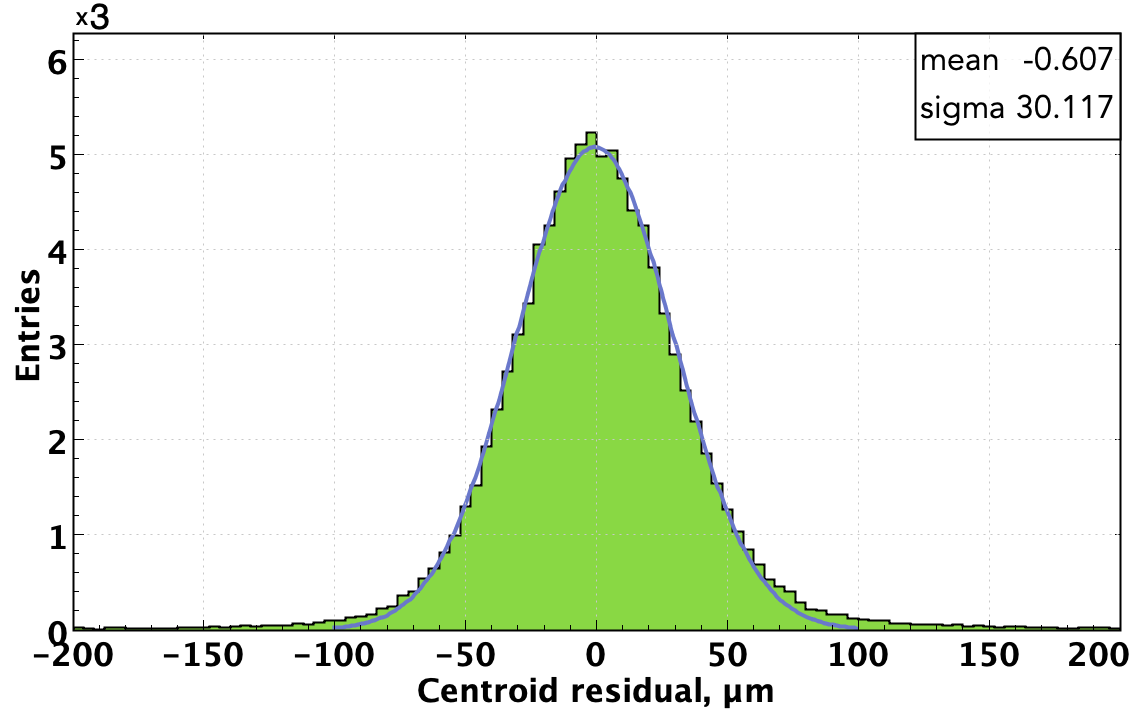
\includegraphics[width=1.0\columnwidth,keepaspectratio]{centroid-residual-mc.png}
\caption{Simulated centroid residual distribution for the SVT module.}
\label{fig:centroid-residual-mc}
\end{figure}

\subsection{Backgrounds, energy deposition, dose rates}

Radiation-induced bulk and surface detector damage studies have been conducted with charged hadrons, leptons, neutrons, and $\gamma$-ray photons. The radiation damage produced by different particles with different energies are scaled under the assumption of the Non-Ionizing Energy Loss (NIEL) hypothesis as the radiation damage in the silicon bulk depends only on the non-ionizing energy loss. The damage caused by different particles is referenced to the damage from 1 MeV neutrons. The standard value for the NIEL of 1 MeV neutrons is 95 MeVmb. 

\begin{figure}[hbt] 
\centering 
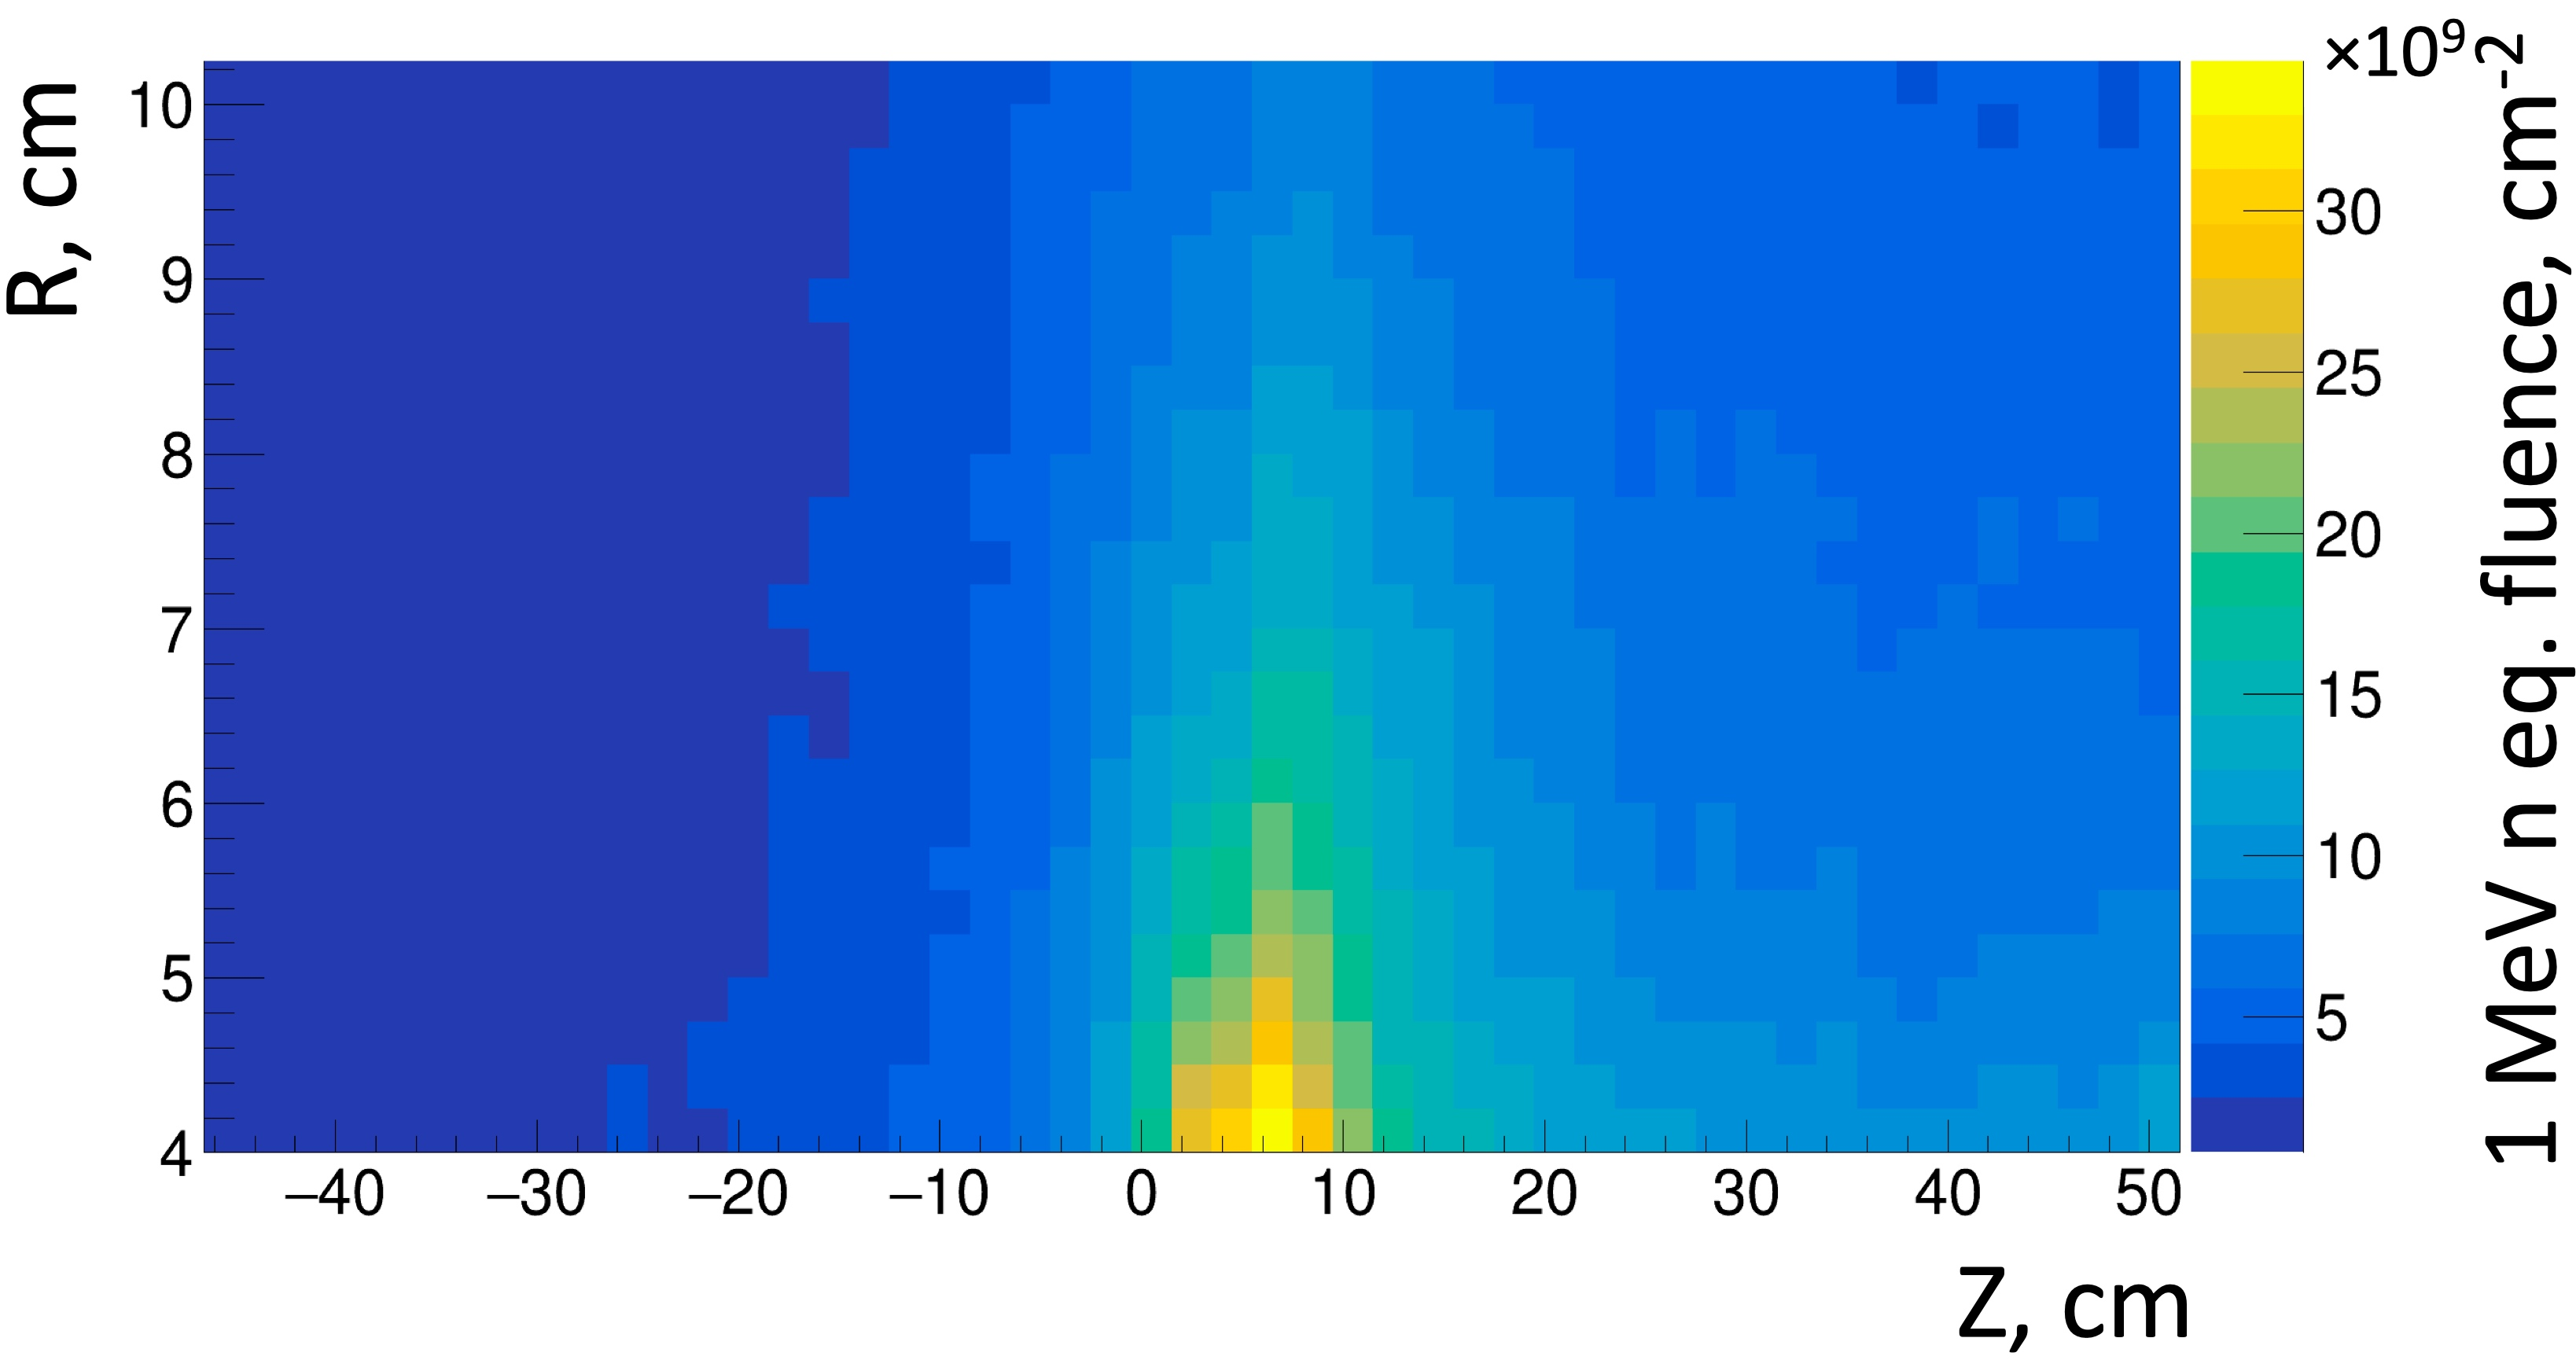
\includegraphics[width=1.0\columnwidth,keepaspectratio]{Pb_1MeVeq.jpg}
\caption{Accumulated 1MeV equivalent neutron fluence for the lead target.}
\label{fig:fluka1}
\end{figure}

To calculate the effects of different target configurations on the SVT detector,  FLUKA~\cite{FLUKA1, FLUKA2} simulations have been performed. In order to include the hadron electro-nuclear production, a dedicated source term has been used to enhance the physics production from the target, since it is a key in radiation estimates for targets with radiation length below 4$\%$. To assess the radiation damage to the SVT, the accumulated 1MeV neutron equivalent fluence has been recorded corresponding to the planned run conditions. For the experiment with lead target, the expected exposure was 240 h at beam current of 38 nA with electron beam energy of 6.6 GeV (Fig.~\ref{fig:fluka1}). For deuterium target, the study has been done for the accumulated charge of 108 mC at 11 GeV (Fig.~\ref{fig:fluka2}). In both scenarios the expected doses should not cause substantial degradation of the silicon sensors.

\begin{figure}[hbt] 
\centering 
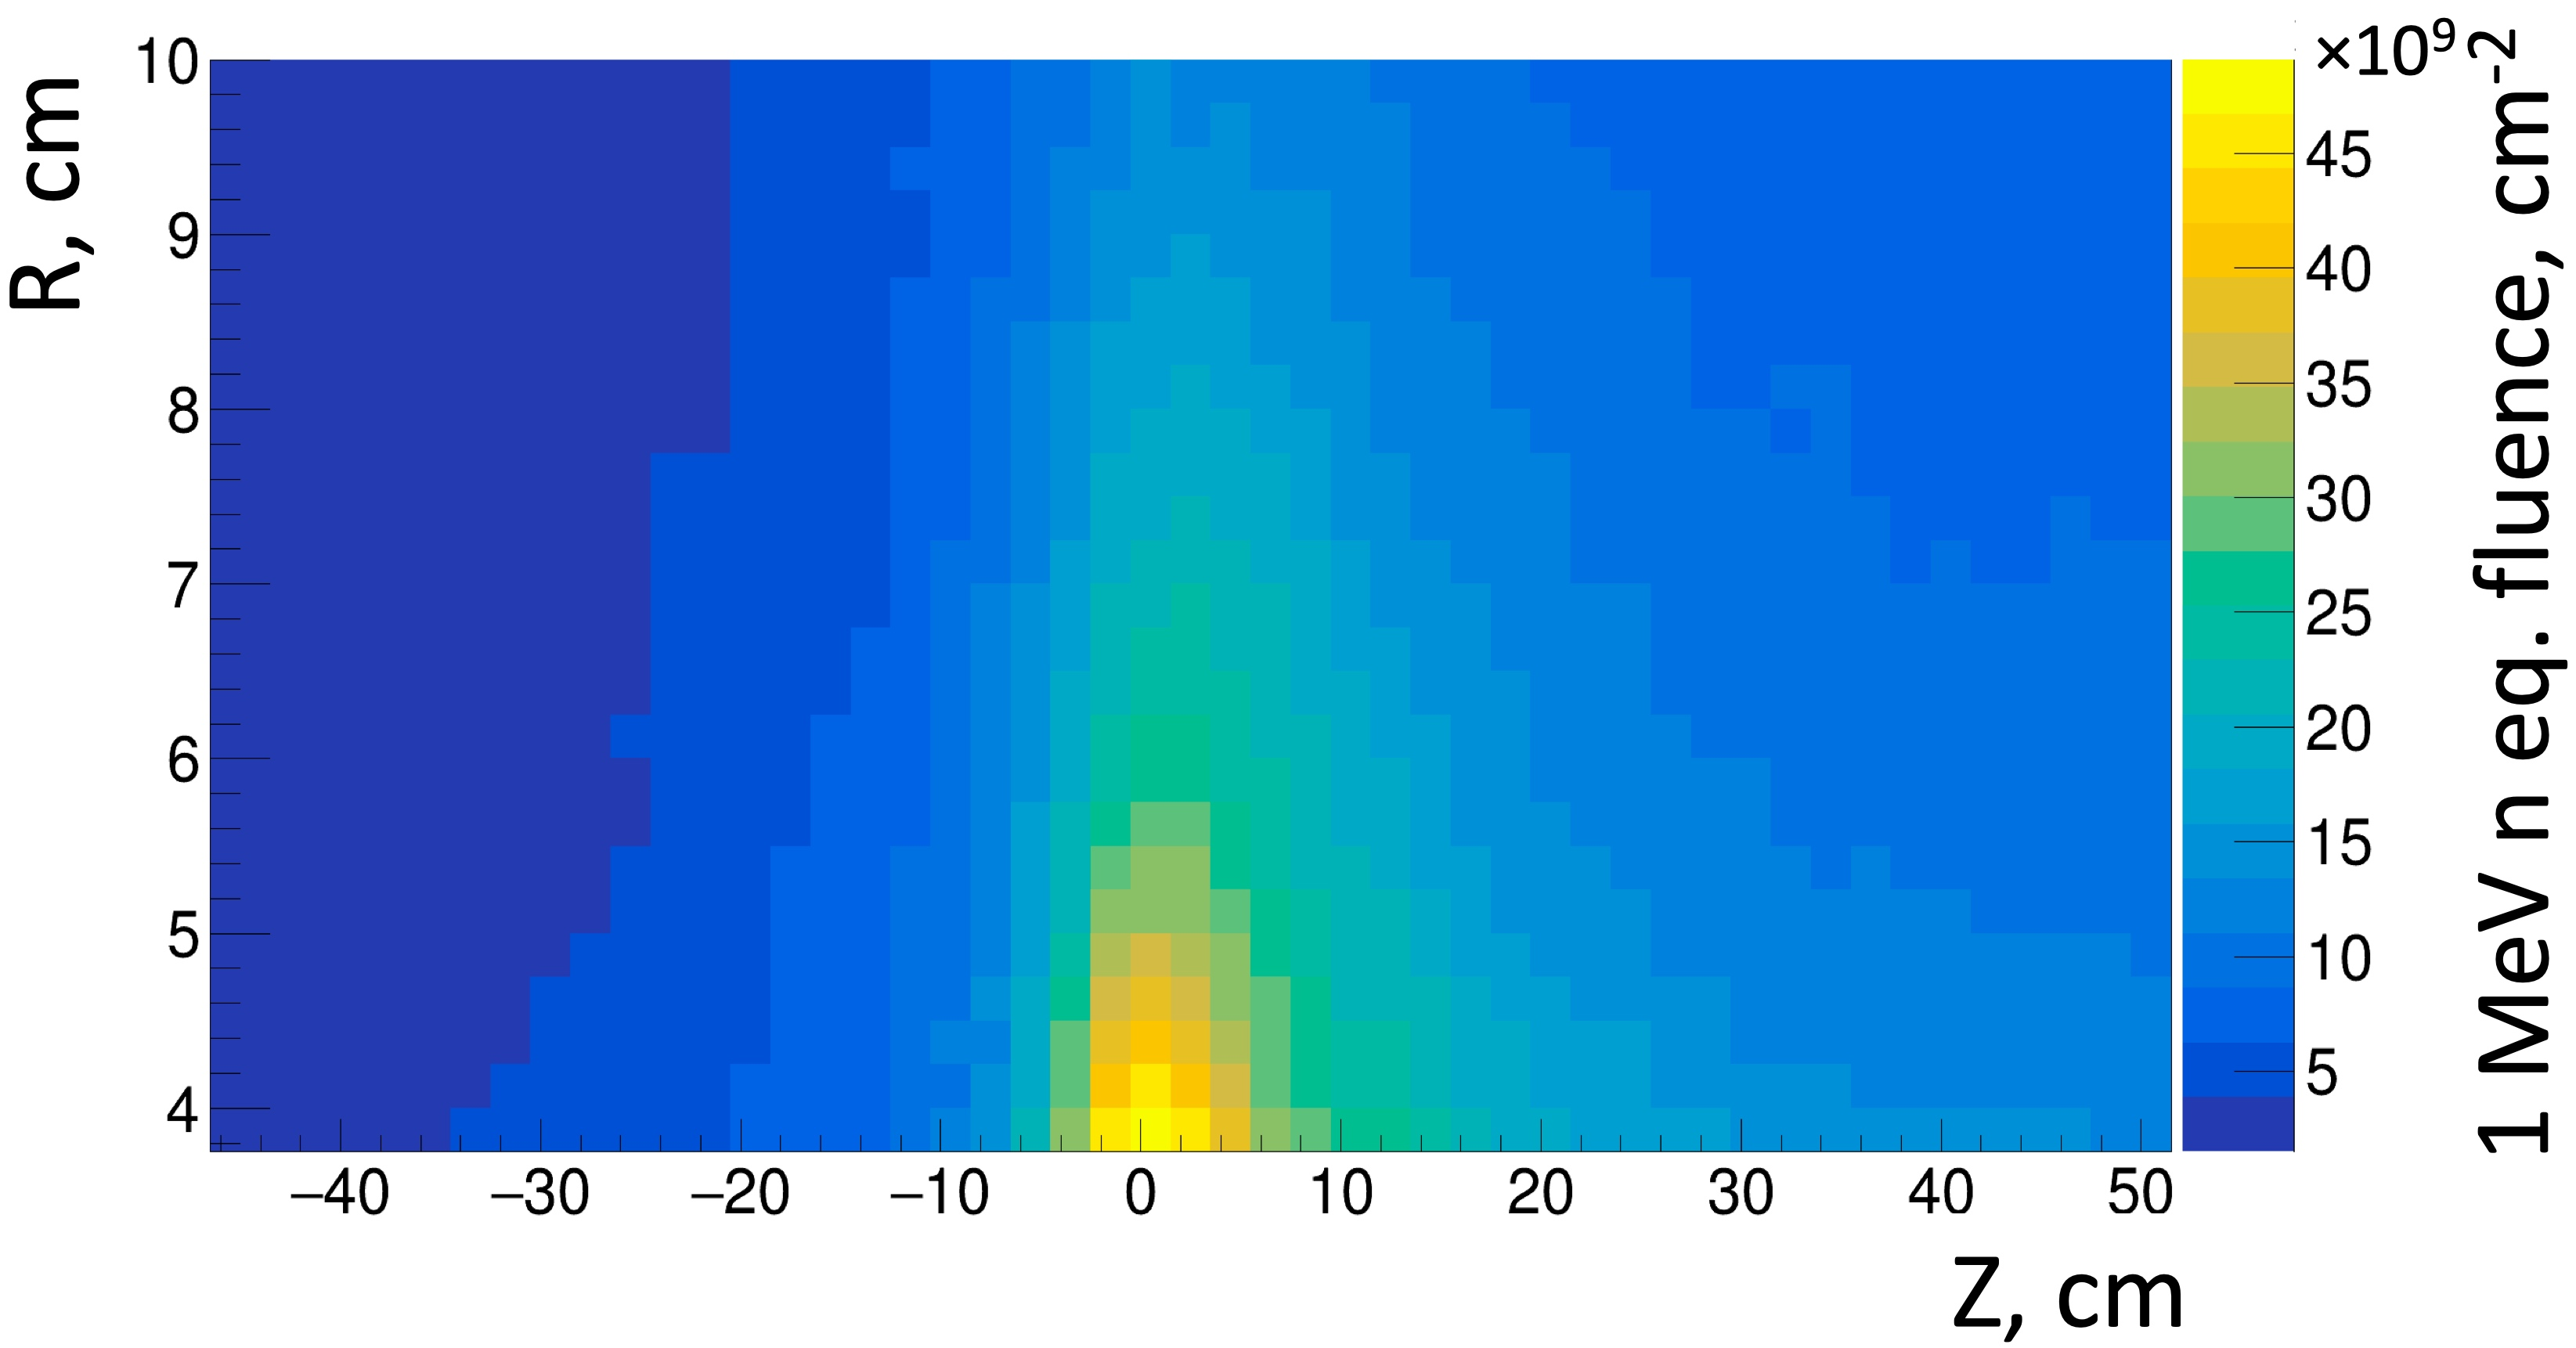
\includegraphics[width=1.0\columnwidth,keepaspectratio]{Deuterium_1MeVeq.jpg}
\caption{Accumulated 1MeV equivalent neutron fluence for the deuterium target.}
\label{fig:fluka2}
\end{figure}

FLUKA simulations of radiation damage levels have been performed in terms of 1MeV equivalent neutron fluence and high energy hadron equivalent fluence which is proportional to the rate of Single Event Effects (SEE)~\cite{FLUKA3}. Estimated levels of radiation damage in radial direction are presented in Fig.~\ref{fig:rad-levels-radial}) for liquid hydrogen and carbon targets at nominal beam currents. Also shown the radiation levels for the tagger magnet yoke during the beam tuning (see the beam line section in this volume).

\begin{figure}[hbt] 
\centering 
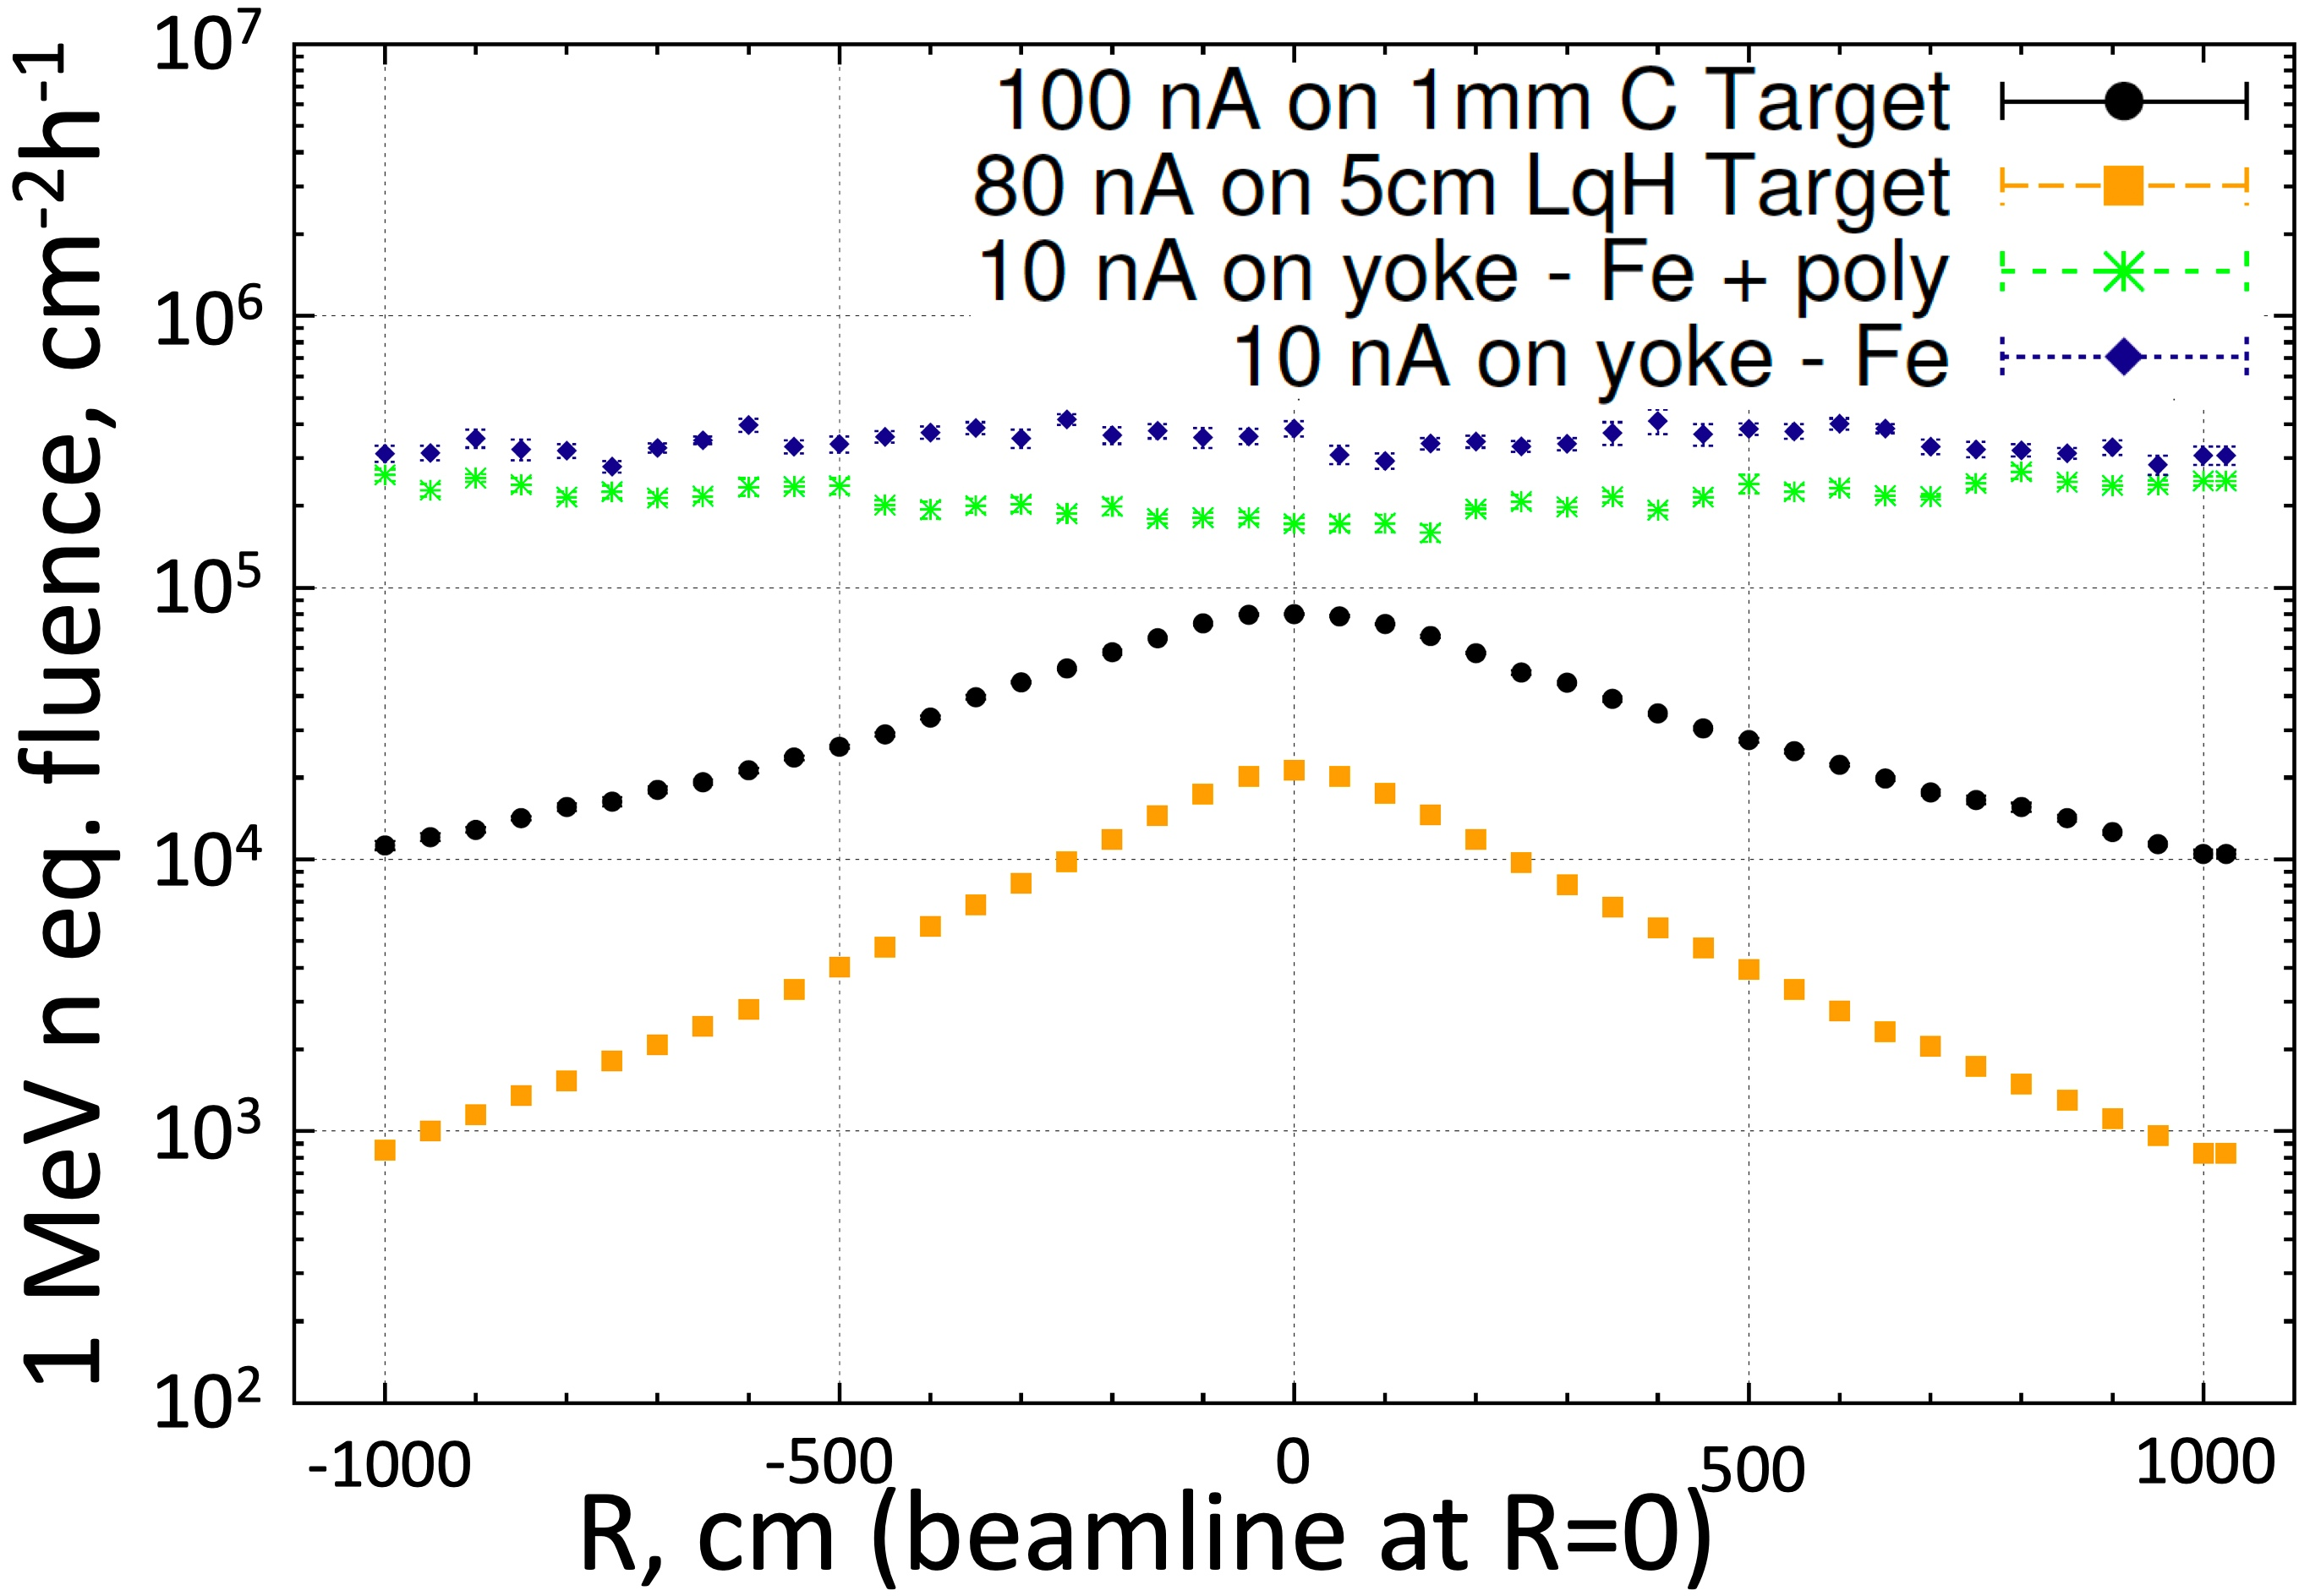
\includegraphics[width=1.0\columnwidth,keepaspectratio]{rad-levels-radial.jpg}
\caption{Estimated levels of radiation damage in radial direction in terms of 1MeV neutron equivalent fluence in silicon.}
\label{fig:rad-levels-radial}
\end{figure}

Simulations of beam-related backgrounds were performed for several thicknesses of a tungsten shielding cylinder around the CLAS12 target covering the first SVT layer. 
 
\begin{figure}[hbt] 
\centering 
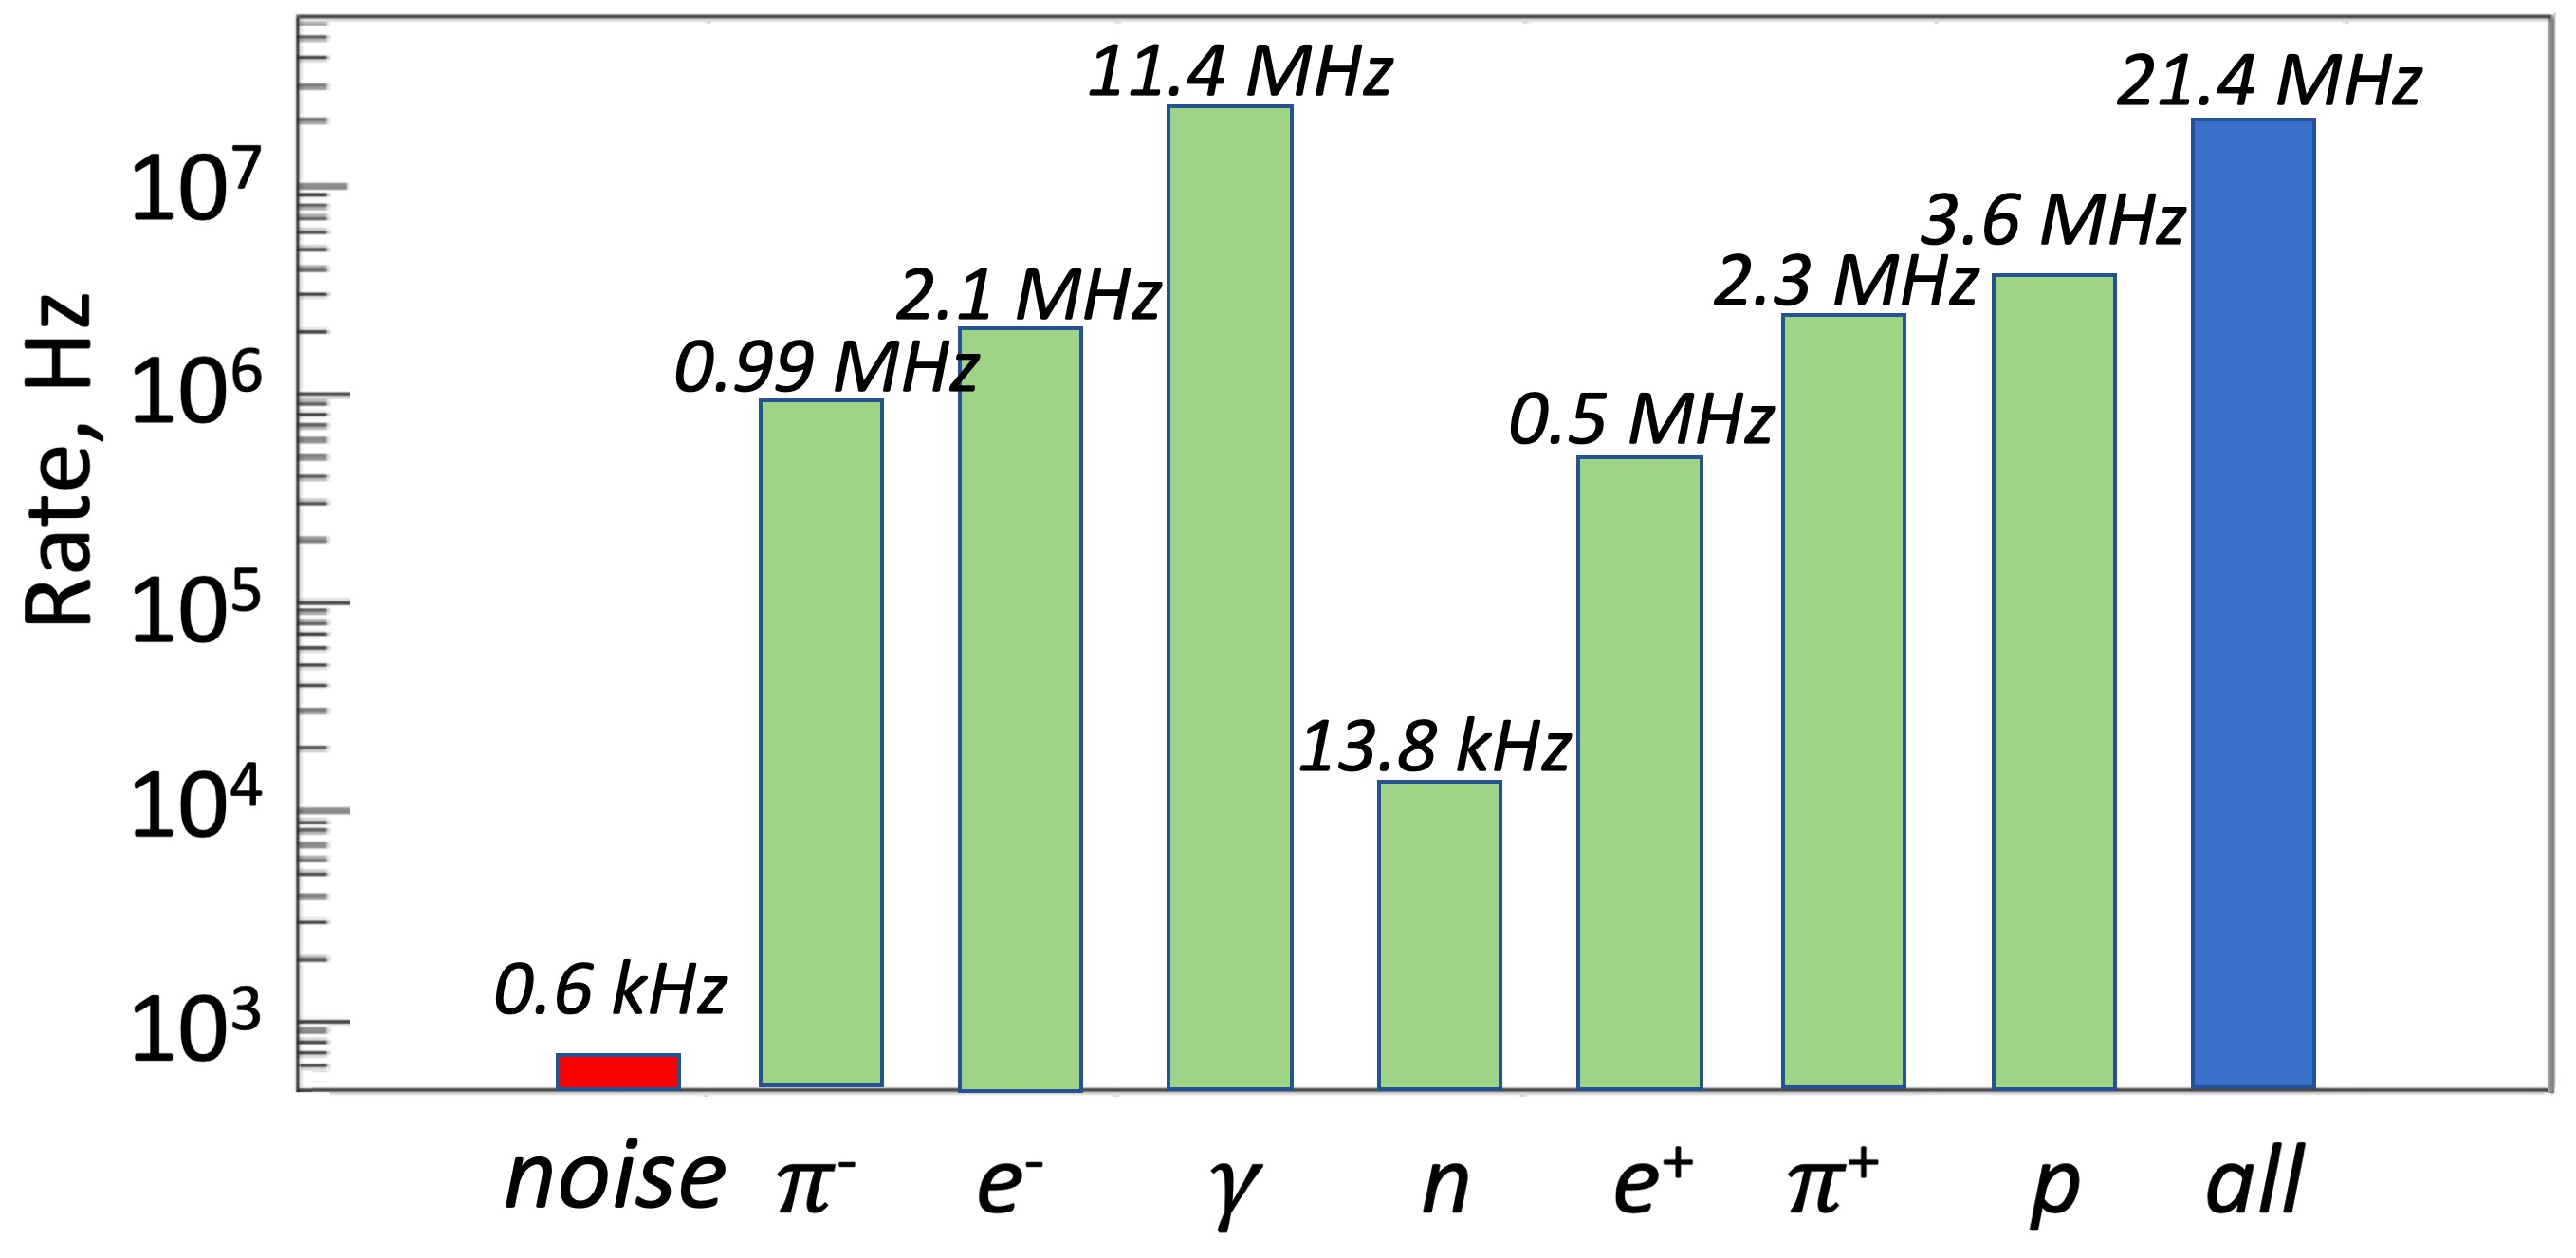
\includegraphics[width=1.0\columnwidth,keepaspectratio]{rates-lh2.jpg}
\caption{Rates in the first SVT layer for a 5-cm long liquid hydrogen target at the nominal CLAS12 operating luminosity of 10$^{35}$cm$^{-2}$s$^{-1}$.}
\label{fig:rates-lh2}
\end{figure}

Fluences, radiation doses, and 1 MeV neutron damage rates in the SVT were calculated for different particles. Rates were estimated for liquid hydrogen, liquid deuterium, carbon, iron, and lead targets. For each event, 124,000 electrons going through the target within a 248.5-ns time window were simulated. This corresponds to the full CLAS12' 10$^{35}$cm$^{-2}$s$^{-1}$ luminosity on a 5-cm-long liquid-hydrogen target at 11 GeV beam energy. Rates in the first SVT layer for a liquid-hydrogen target are shown in Fig.~\ref{fig:rates-lh2}. For carbon target at a threshold of 40 keV the hadronic rate was estimated to be 5 MHz (total rate 40 MHz) with strip hit rates of 3.1 kHz (region 1), 2.2 kHz (region 2), and 1.7 kHz (region 3). The energy deposited in layer 1 for the electromagnetic and the hadronic particles is shown in Fig.~\ref{fig:energy-deposited-l1}. At a threshold of 30 keV, 92$\%$ of the electromagnetic background is rejected while preserving  99.5$\%$ of the signals coming from the hadrons~\cite{TDRSVT}.

\begin{figure}[hbt] 
\centering 
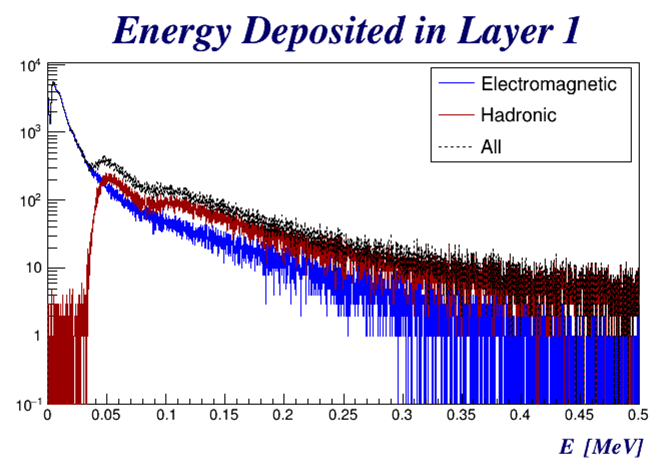
\includegraphics[width=1.0\columnwidth,keepaspectratio]{energy-deposited-l1.png}
\caption{Energy deposited in the SVT layer 1 for electromagnetic and hadronic particles for a liquid hydrogen target at the nominal CLAS12 operating luminosity.}
\label{fig:energy-deposited-l1}
\end{figure}

A tungsten shield 51~$\mu$m thick is installed on the target scattering chamber. The shield consists of 2 sheets mounted over the top and bottom halves of the foam cylinder referenced to the SVT common ground. The SVT rates and radiation damage benefit from the inclusion of the tungsten shield. The rates have been compared with physics run data at several beam currents.

While the gamma fluences / doses show a dramatic decrease with the introduction of shielding, the total fluences and doses decrease significantly for the thinner configuration and do not vary much for thicker tungsten (see Fig.~\ref{fig:rates-l1}). The photon radiation dose becomes negligible for 50 $\mu$m or more of tungsten with total 1 MeV equivalent radiation dose about 65 krad per year on a liquid-hydrogen target. For 15 years of running the experiment on a carbon target the estimated radiation dose for the sensors is 2.5~Mrad (with 50 $\%$ operation) \cite{TDRSVT}. 

\begin{figure}[hbt] 
\centering 
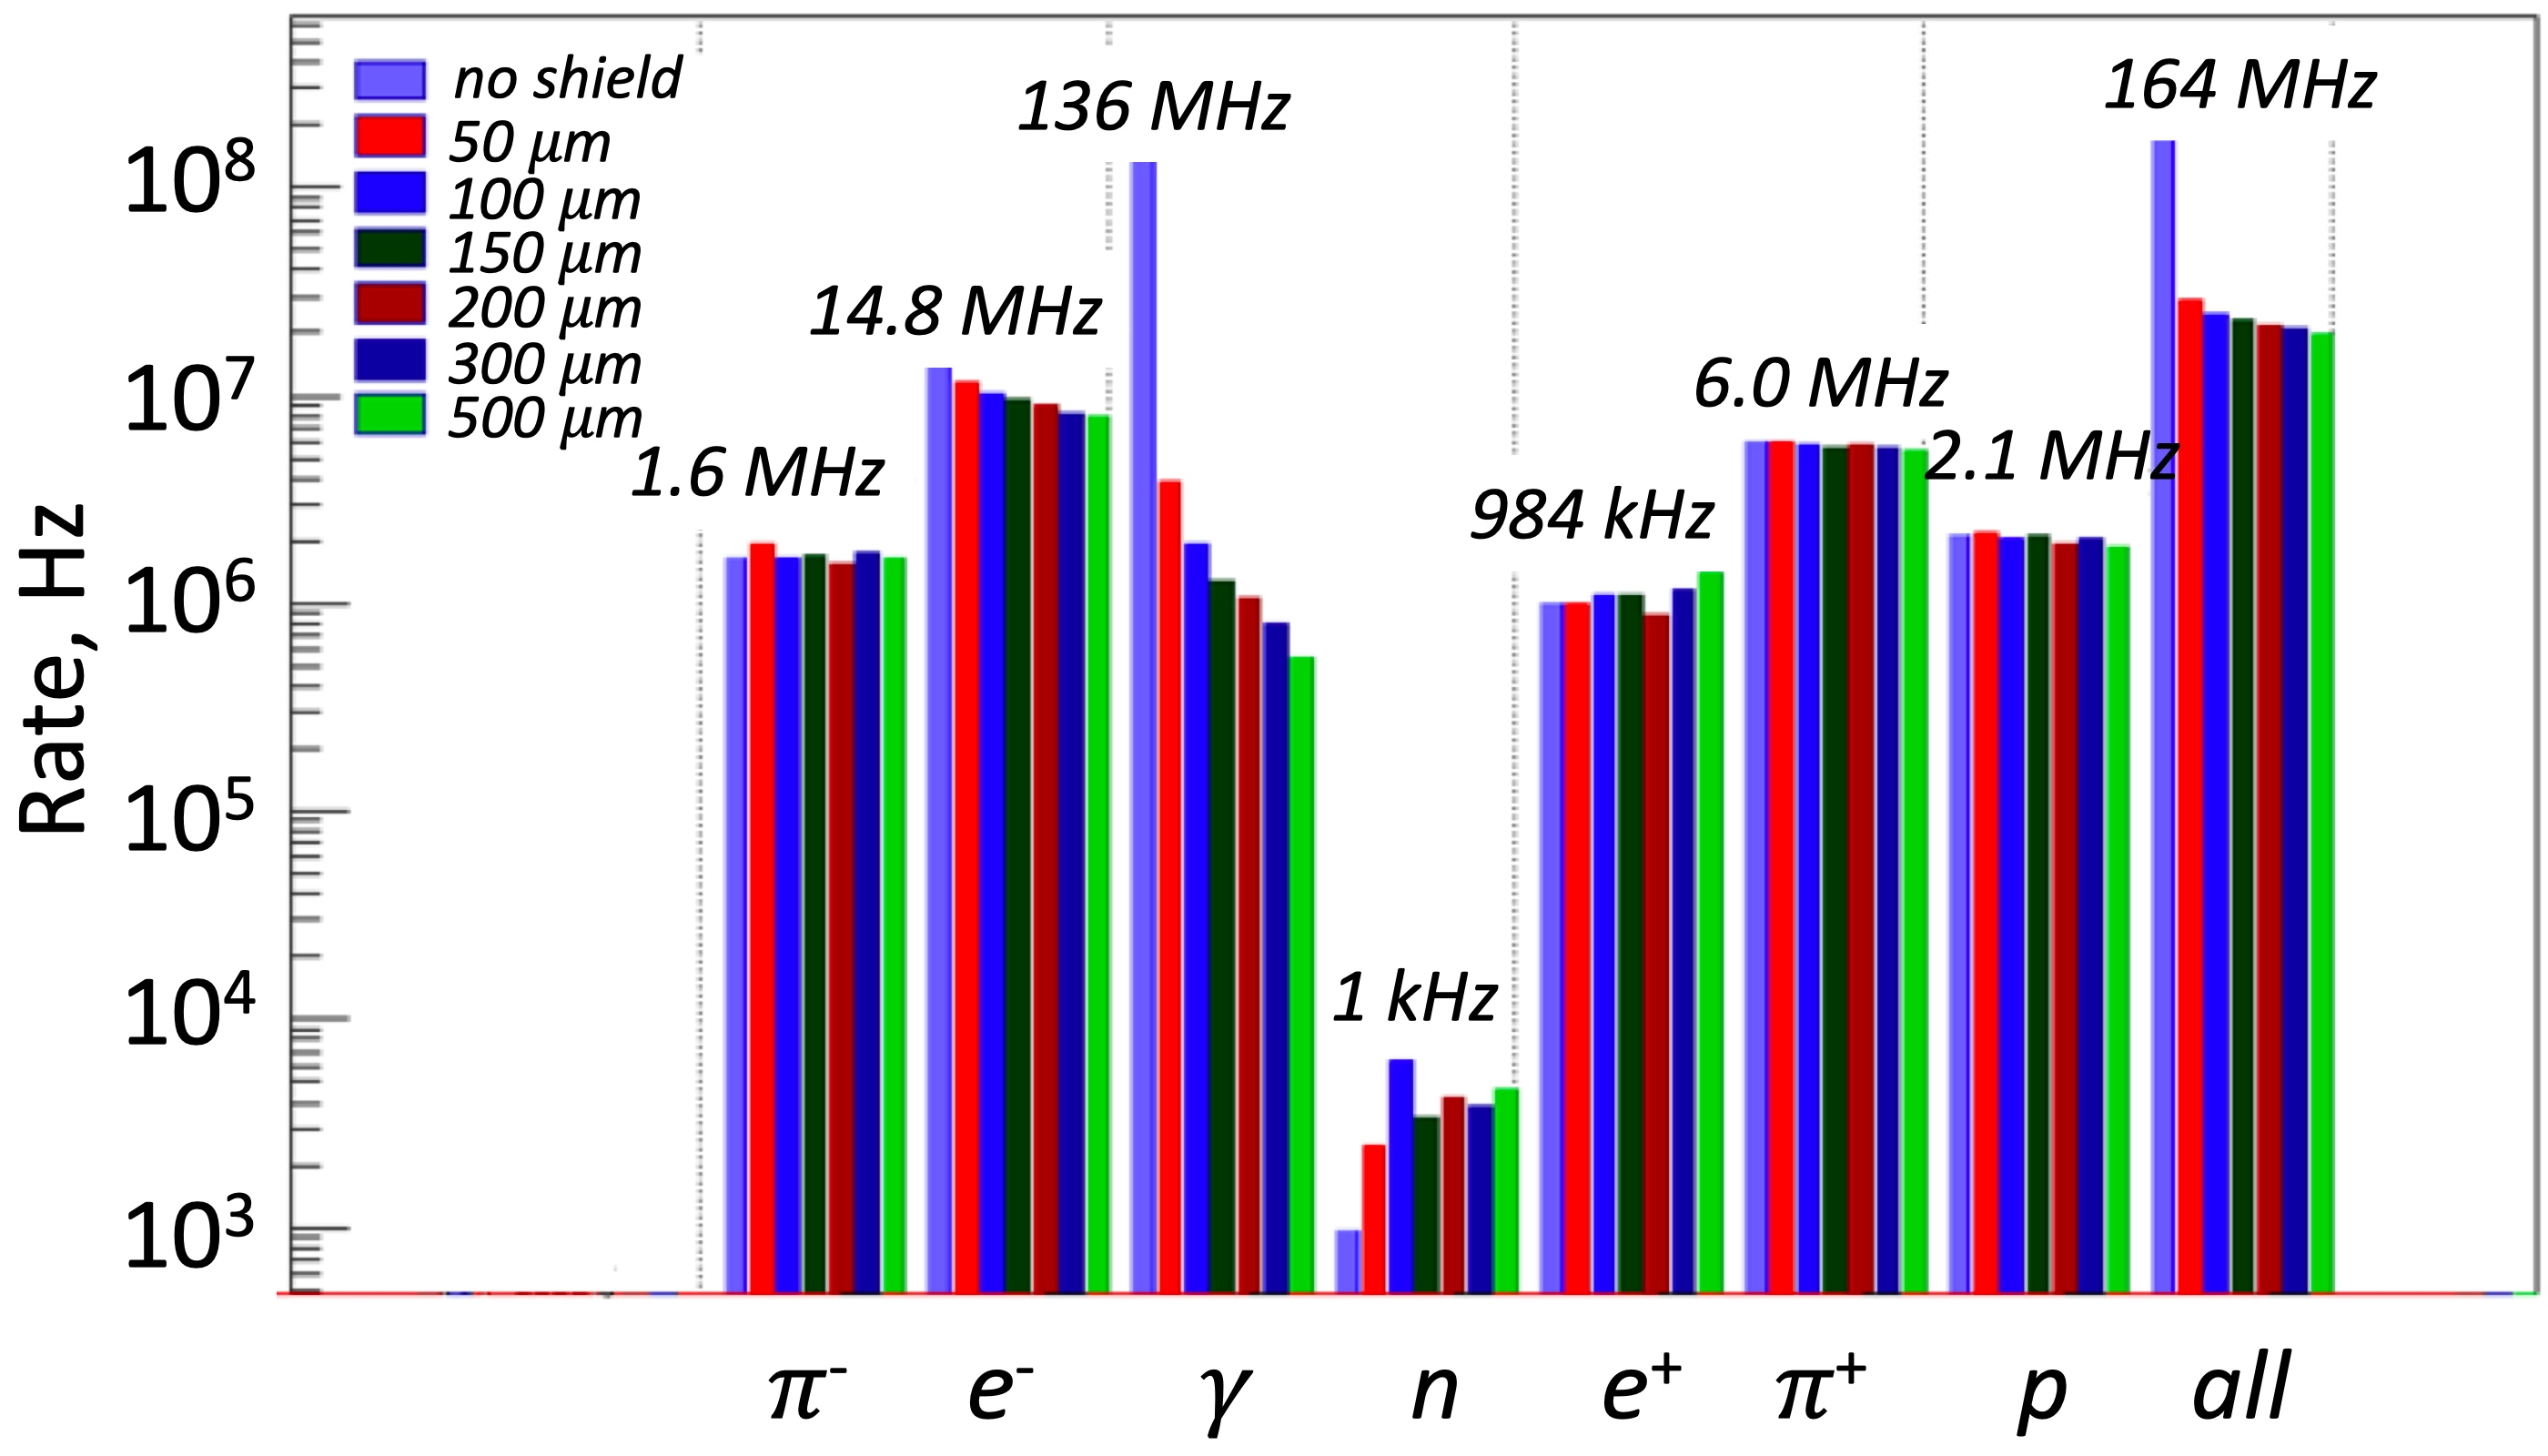
\includegraphics[width=1.0\columnwidth,keepaspectratio]{rates-l1.jpg}
\caption{Rates in the first SVT layer for different tungsten shield thickness from 50 to 500 $\mu$m for a liquid hydrogen target at the nominal CLAS12 operating luminosity. No energy threshold cut applied.}
\label{fig:rates-l1}
\end{figure}

An estimate of the double hit rate was performed. Fig.~\ref{fig:double-hit-rate} shows the probability of the double hits in the inner region of the SVT. The ratio of the double hits to the single hits was found to be about 1$\%$.

\begin{figure}[hbt] 
\centering 
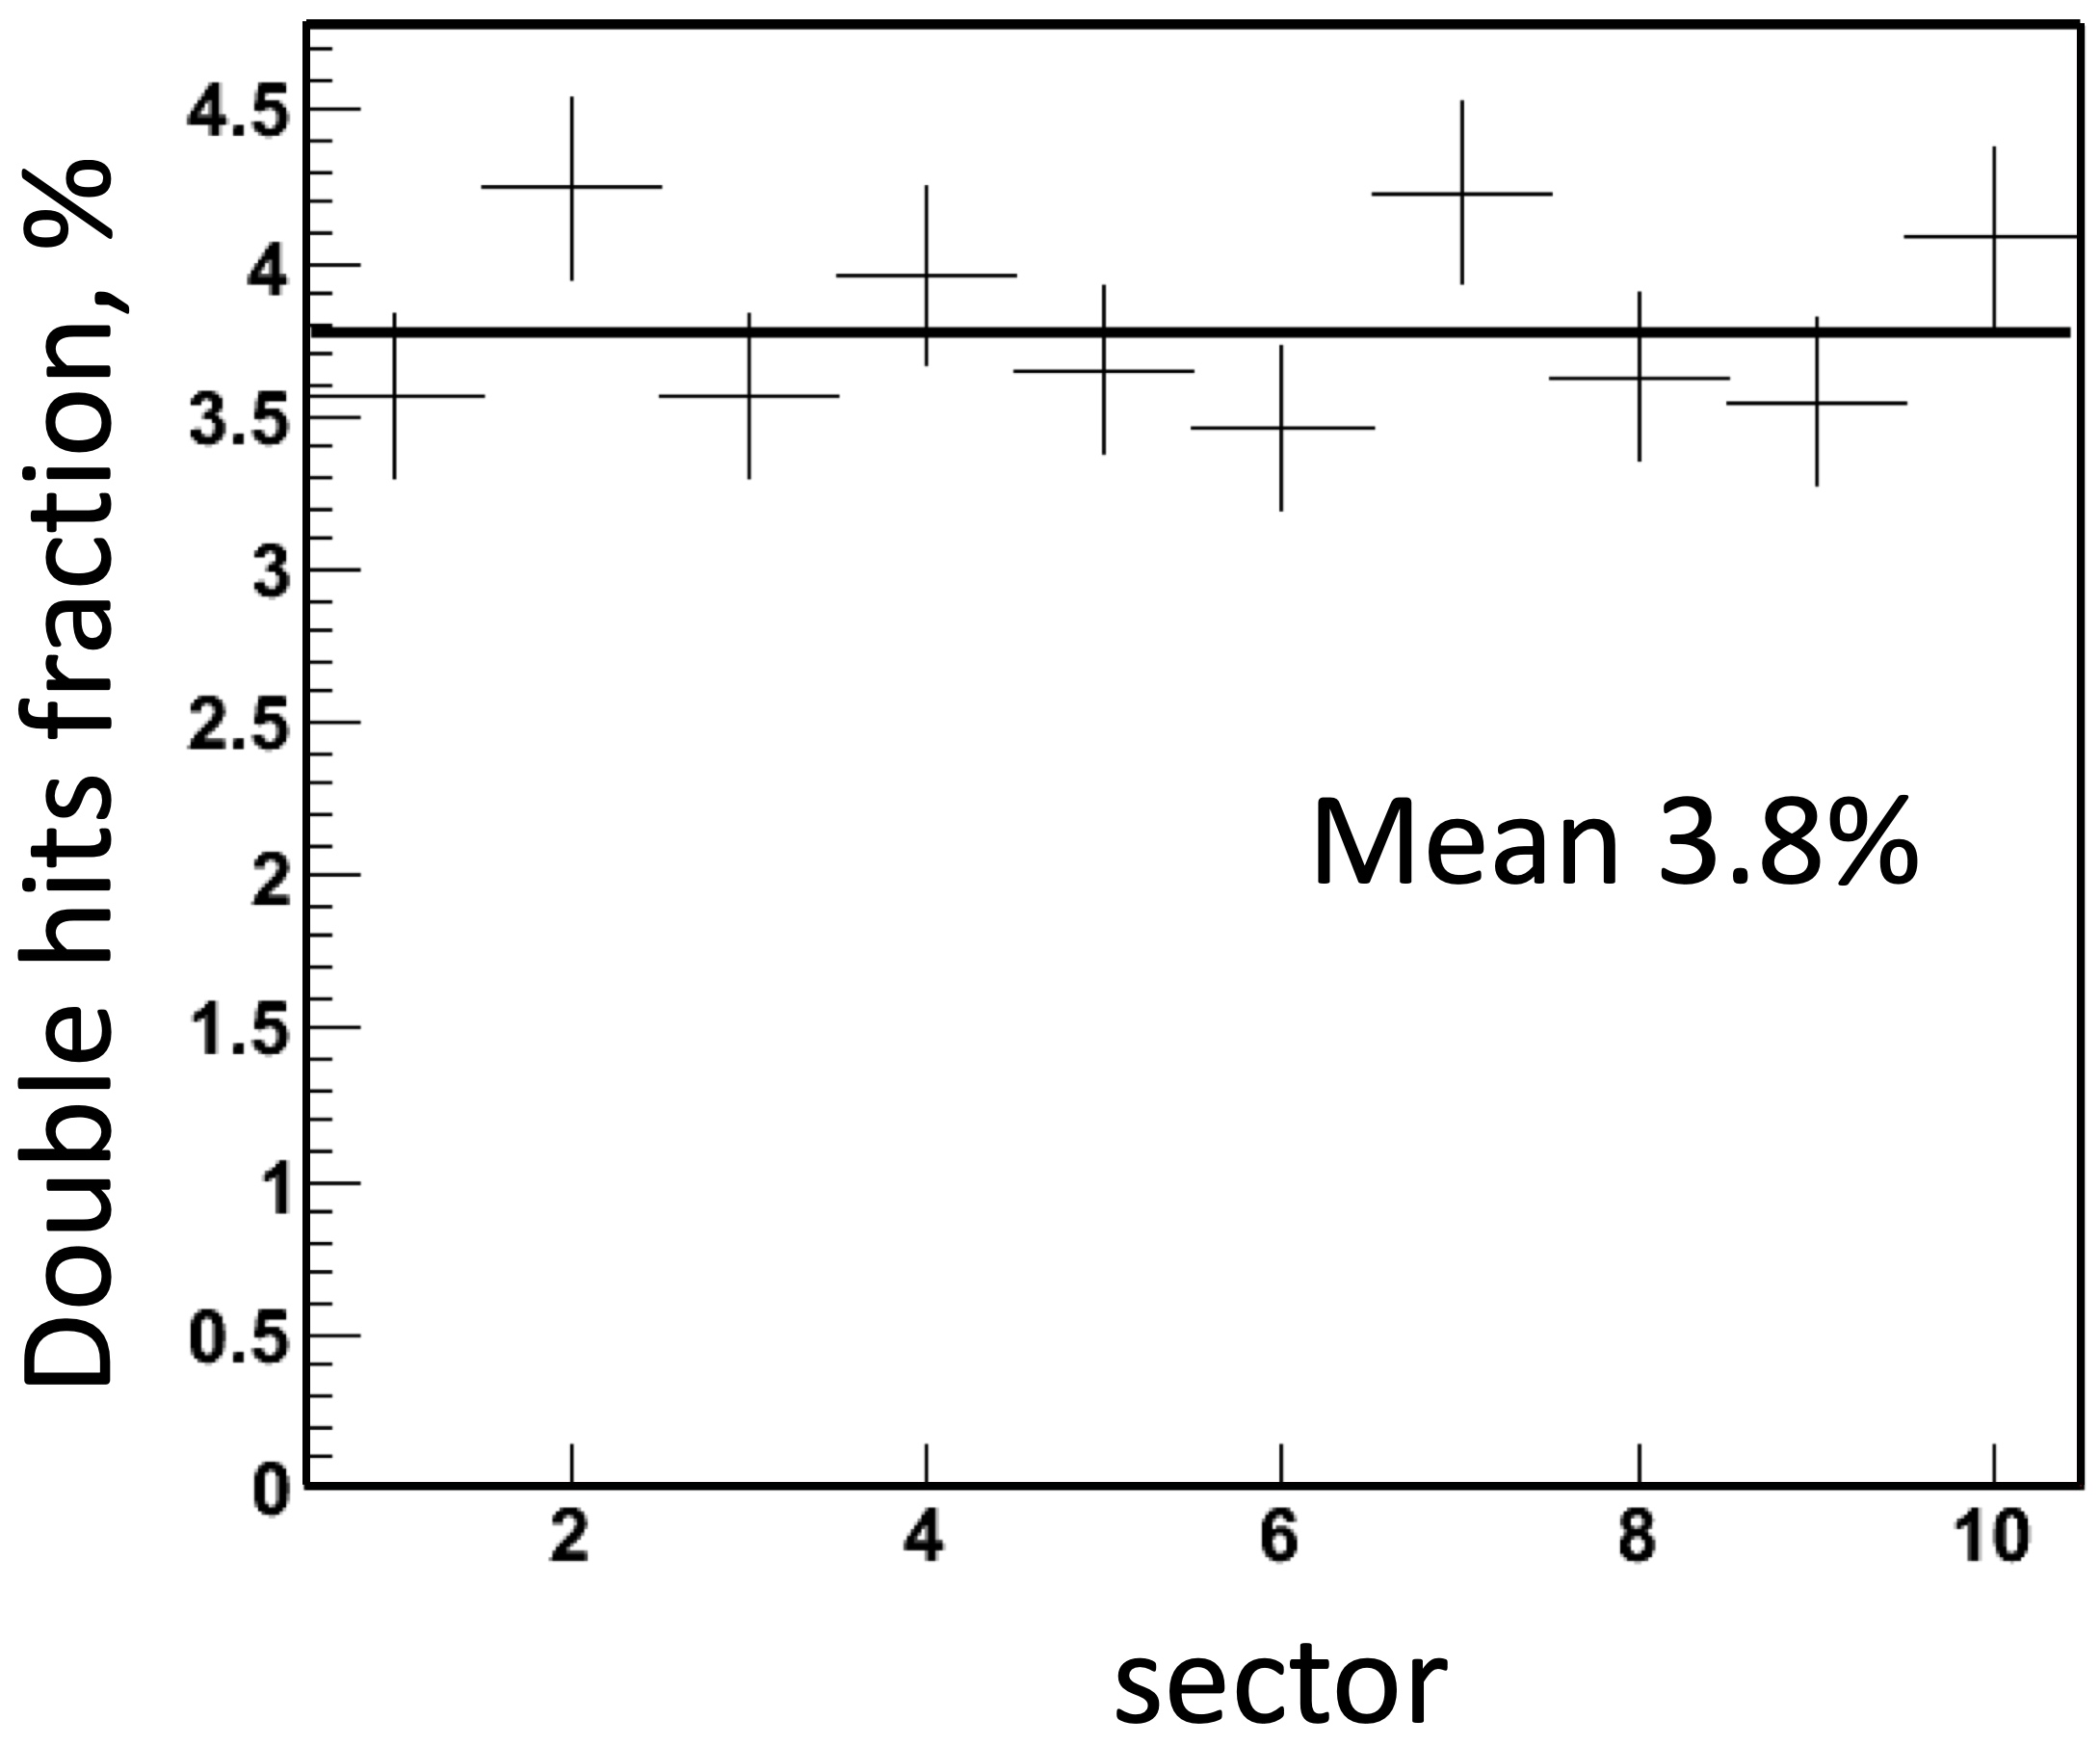
\includegraphics[width=1.0\columnwidth,keepaspectratio]{double-hit-rate.jpg}
\caption{Double hit fraction in the region 1 with liquid hydrogen target.}
\label{fig:double-hit-rate}
\end{figure}

\subsection{Magnetic Field}

Due to the constrains on the maximum length of the cables, the readout, slow controls, and power supply crates are installed on a movable service cart within few meters from the detector. To assess the potential impact of the solenoid field on the SVT DAQ, a magnetic field map was simulated for the location of the power supply and readout crates. Fig.~\ref{fig:solenoid-field}) shows that the maximum strength of the field for the crates is at an acceptable level of 100 G.

\begin{figure}[hbt] 
\centering 
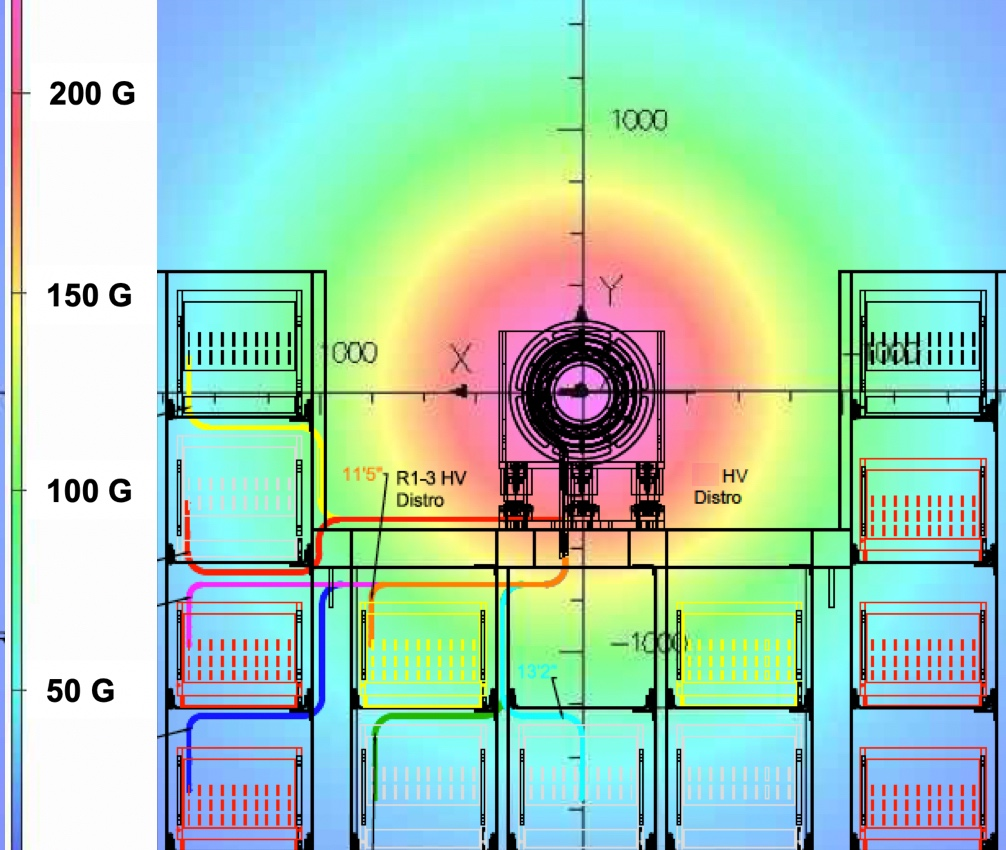
\includegraphics[width=1.0\columnwidth,keepaspectratio]{solenoid-field.jpg}
\caption{Solenoid field map at the location of the SVT service cart.}
\label{fig:solenoid-field}
\end{figure}




\section{Trigger System Firmware Development}

After generic Trigger System design was complete and the hardware components entered their production stage, the firmware development began. Both HLS and VHDL tools were used. Work was performed using data samples generated by the CLAS12 GEMC/GEANT4 package and cosmic data after the hardware components were installed. This section describes our procedures. Additional development and validation with beam are described in Section \ref{sec:validation}.

\subsection{Preparation of Simulated Data Sets}
\label{simulated_data_preparation}

Simulated data sets for Trigger System development were prepared using GEMC (GEANT4-based CLAS12 simulation package \cite{gemc-ref}). GEMC has a fully realistic CLAS12 geometry description and complete maps of the magnetic field, and produces digitized results suitable to be converted into the pre-trigger data format.

Various data sets were generated depending on what was needed for the development of particular trigger components. For example, fixed energy single electron sets were produced for the initial development of the EC and PCAL components. For these data sets, all detectors positioned upstream of the EC or PCAL were disabled to make sure the single electron directly hit the EC or PCAL. In this way the cluster finding algorithm could be developed and tested in ideal conditions. After that, realistic data samples were produced and the algorithm was tested again.

Another data set was used to create the road dictionary for the Drift Chamber-based trigger component.  For this purpose, positive and negative tracks were generated uniformly  in a selected momentum, $\theta$ and $\phi$ range and tracked through the CLAS12 detector to determine the list of DC wires involved by the particle trajectory. More details can be found in Section \ref{dc_dictionary}.


\subsection{Development Using Simulated Data}

The trigger development process consisted of several methods that depended on the nature of the trigger component. Most Stage 1 components were implemented using the HLS/VIVADO tool, where the firmware was written using an HLS C++ extension. In that case, it was possible to develop and validate the firmware as part of the offline reconstruction framework using a standard desktop computer. Usually the offline processing alghorithms were re-written using HLS/C++, with appropriate simplification and structural changes to make it suitable for the FPGA firmware. Simulated data were used as input, which were processed directly by the HLS/C++ code and compared with the initial simulation parameters. In addition, the same samples were processed by the offline reconstruction software and the results were compared with the trigger output. This double-check method practically guarantees bug-free implementation. There was no single case when the C++ implementation passed tests on the simulated data and then failed during the final validation stage. The most complicated Stage 1 components were developed and tested using this method.

Several components of the trigger were written mostly in VHDL and initially no software existed for feeding GEMC data into the HDL simulations. This was the case for the Stage 1 FT and DC tracking trigger, as well as the Stage 2 and Stage 3 components of the trigger. These modules relied on standard VHDL test benches to feed/generate test vectors for evaluating the correctness of the design modules. For example, the FT test bench generated clusters at each position of the calorimeter and hodoscope to test the channel mapping and geometry matching. Additional specific test cases verified the FT trigger clustering time coincidence, cluster multiplicity, and latency to ensure it operated as expected. C/C++ modules were written that emulated the FT the DC tracking trigger so the algorithms could work in the same offline framework as described above for the other Stage 1 components.

\subsection{Development and Validation Using Cosmic Data}

When the hardware components for the CLAS12 detector were constructed and mostly installed, and the first version of the firmware was ready for testing, all three Trigger System firmware stages were loaded and development continued for the entire Trigger System using cosmic data. At that point we started to perform Trigger System validation for some components, while development was continued for others, as described in the following sections.

\subsubsection{Alternative 'Hit-Based' Trigger System}

The CLAS12 detector inheritated some components from the original CLAS detector (see \cite{clas-nim}), in particular its Trigger System. That system was fed by TDC/discriminator boards and was able to produce ``hit-based'' information only (i.e. based only on the list of channels above threshold). We decided to keep it for reference purposes as an alternative to the new Trigger System. It was used during CLAS12 cosmic data detector calibrations and validation of the new Trigger System up to the point when new Trigger System was ready. It is still operational and can be used to double-check the main CLAS12 Trigger System if needed.

\subsubsection{Development and Validation of ECAL Special Purpose Trigger with Cosmic Data}

The first detector calibrations employed cosmic data. Here we will describe, as an example, one of the procedures related to EC/PCAL calibration needed for correct Trigger System performance. Similar procedures were executed for all detectors participating in the Trigger System.

The efficiency and spatial uniformity of the cluster finding trigger in the EC/PCAL described in Section \ref{sec:ECAL} requires already calibrated calorimeters with pre-determined PMT gain and light attenuation constants loaded into the VTP/FPGA trigger firmware.  Calibration runs using a special purpose MIP trigger were used to obtain these constants. For that purpose a so-called ``pixel trigger'' was developed and loaded into the Stage 1 firmware along with the main trigger, so it was possible to calibrate the system using a pixel trigger and then switch to the main one for data taking. This ``pixel trigger'' used a simple multiplicity condition on 1D cluster size for each U,V,W view to reject undesirable muon trajectories and select normally incident tracks.  This reduced the trigger and data rate by 95$\%$ and ensured the same MIP energy was deposited for all possible triple intersections of single strips.

The pixel trigger pipeline executes these steps in parallel, with user configurable parameters in bold:
  1) If FADC hit energy $>$ \textbf{EMIN}, make a pulse \textbf{HITWIDTH}*4~ns for that strip.
  2) Look for coincidences of U,V,W pixel strip candidates from step 1.
  3) Evaluate multiplicity \textbf{EVALDELAY}*4~ns clock cycles after the leading edge of a candidate pixel from step 2.
  4) Generate a pixel trigger if the multiplicity requirement is met and we still have a hit on U, V, and W. 

Additional configurable trigger elements were introduced, including a total energy sum threshold \textbf{ESUM} and a look-up table for triplets of strips that satisfy the geometrical constraint $dU+dV+dW=\textbf{DALITZ}$, where $d$ is the normalized distance to the hit strip indicated by the arrows in Fig.~\ref{fig:pcal_cosmic_1} and $\textbf{DALITZ}=2$ for perfect pixels.  The latter test was sometimes necessary to prevent noisy PMTs from saturating the multiplicity (N=3) trigger condition.  Offline analysis showed that about $90\%$ of pixel triggers satisfied the Dalitz test (see Fig.~\ref{fig:ec_offline}), while adjacent calorimeter elements that did not use the trigger had a much smaller pixel fraction.  This suggests the pixel trigger helps to suppress events that undergo multiple scattering, which would trigger adjacent strips and violate the multiplicity requirement.

\begin{figure}[!htb]
 	\centering
  	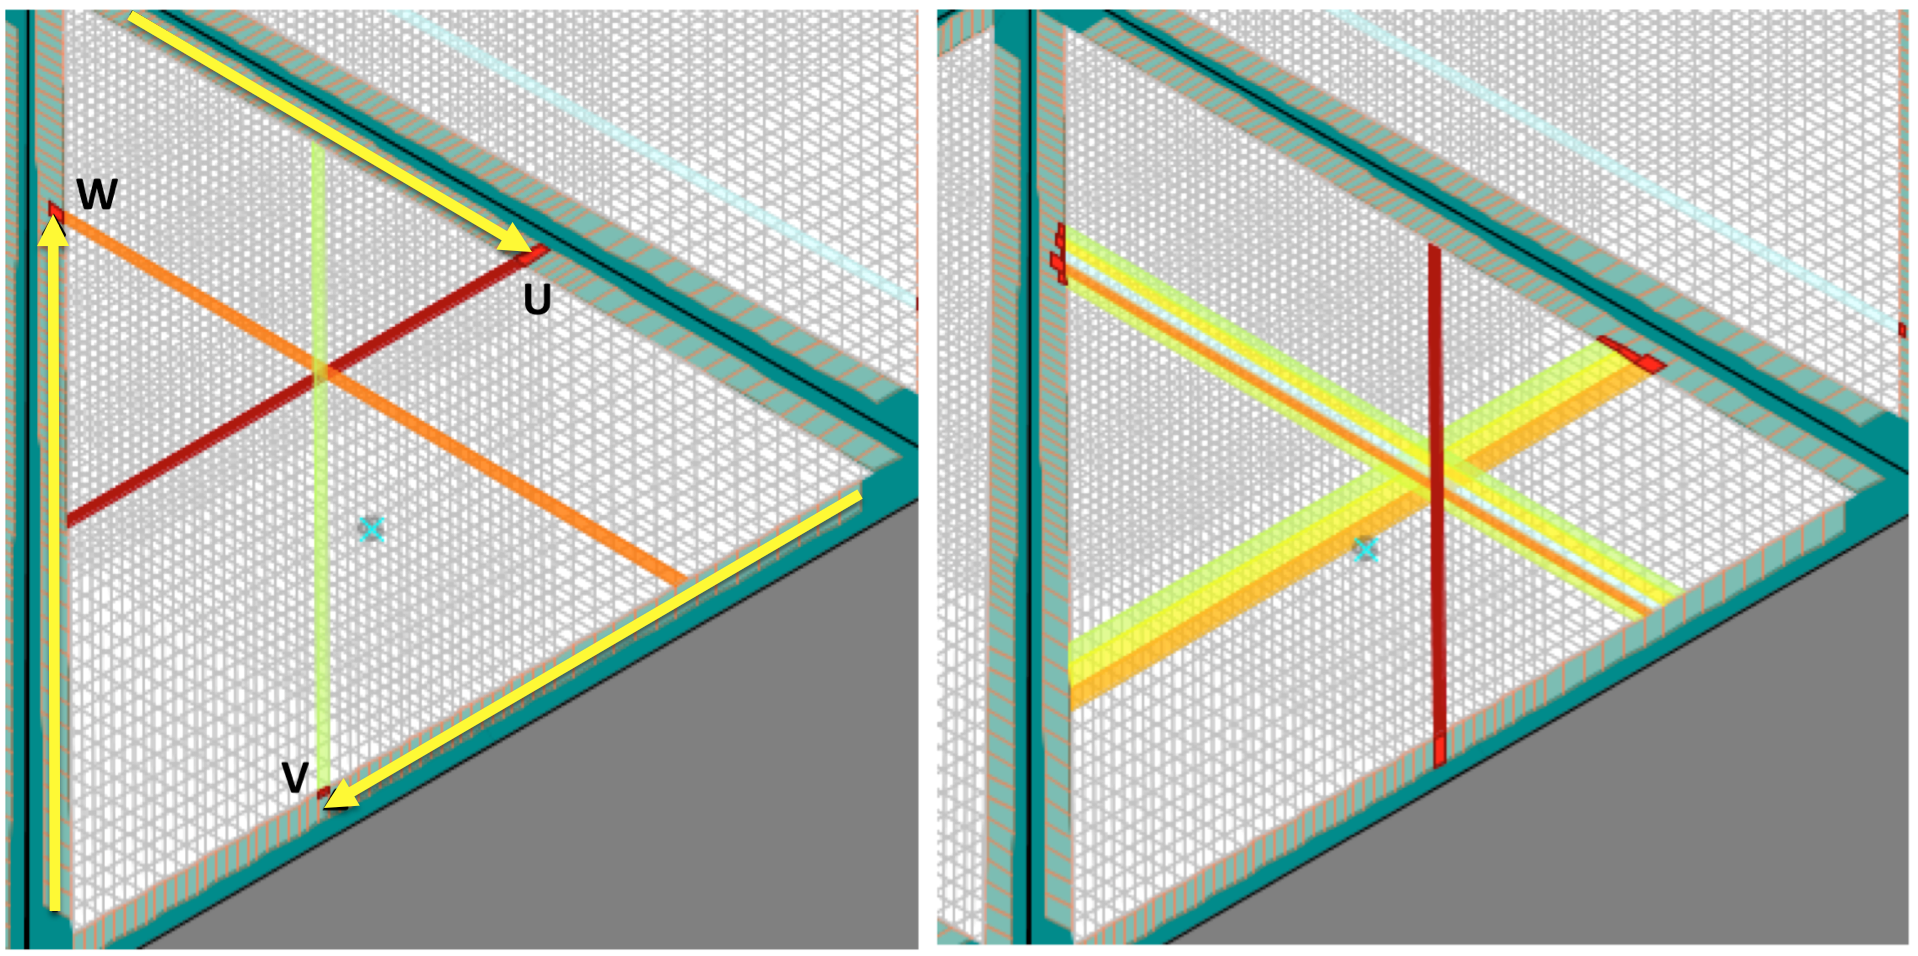
\includegraphics[width=0.95\columnwidth,keepaspectratio]{img/TwoClusters.png}
 	\caption{Examples of clusters from cosmic muon triggers.  The desired trajectory (left) is normally incident on the face of PCAL and satisfies the single pixel multiplicity condition (N$_u$=N$_v$=N$_w$=1) in the FPGA pixel trigger. The event at right shows a more vertical trajectory rejected by this trigger.}
	\label{fig:pcal_cosmic_1}
\end{figure}

\begin{figure}[!htb]
 	\centering
  	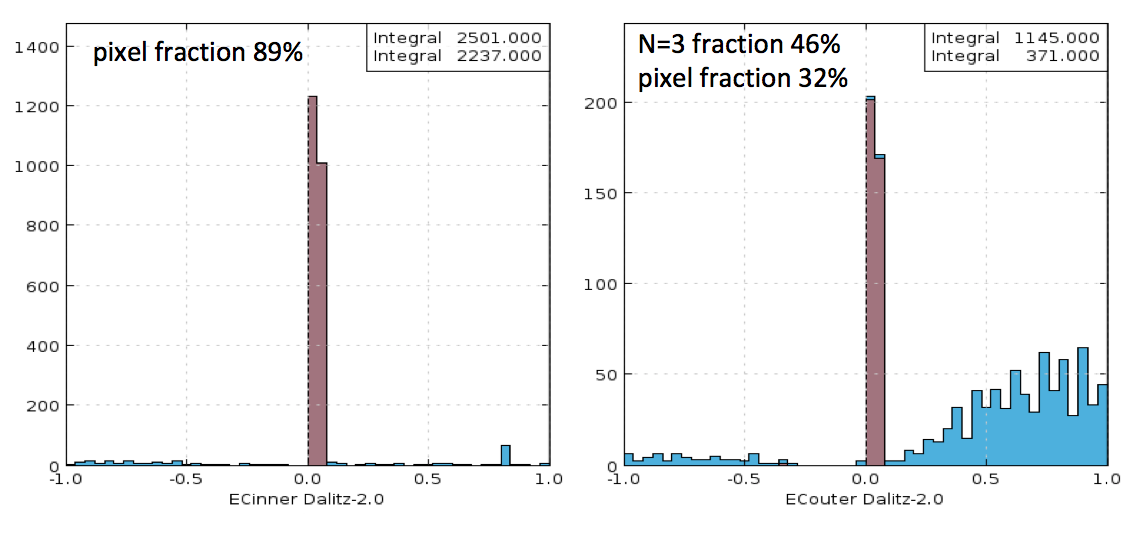
\includegraphics[width=1.0\columnwidth,keepaspectratio]{img/PixelFraction.png}
 	\caption{Offline analysis of events that satisfied the pixel trigger in the $EC_{inner}$  calorimeter.  Left plot shows 89$\%$ of $EC_{inner}$  triggers satisfied the pixel test $dU+dV+dW=2$.  Right plot shows only 14$\%$ of the $EC_{inner}$ triggers found an $EC_{outer}$ event that satisfied both the $N=3$ and pixel test.}
	\label{fig:ec_offline}
\end{figure}


\subsubsection{Development and Validation of DC Component of the Trigger System with Cosmic Data}

Early tests of the Drift Chamber tracking trigger were done using cosmic events triggered from the ECAL. A small fraction of events had tracks near the target location where the road dictionary was defined, but within a day enough statistics could be collected to do checks that the tracking trigger was functioning. Offline reconstruction of events with reconstructed tracks were checked to see if the tracking trigger fired as shown in Fig.~\ref{fig:dc_cosmic_efficiency}. Any events with tracks that passed through the target, but failed to be tagged by the tracking trigger were run through simulations to identify the reason. The tests clearly showed very loose acceptance and motivated tighter kinematic constraints on the dictionary generation that were eventually done when studies with beam were later performed.

\begin{figure}[!htb]
 	\centering
  	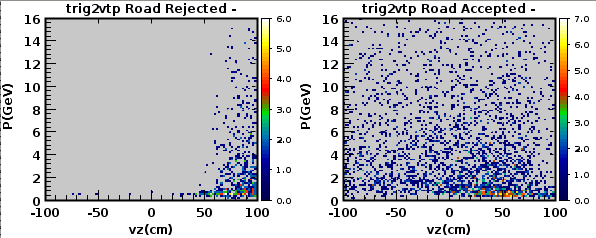
\includegraphics[width=1.0\columnwidth,keepaspectratio]{img/dc_cosmic_efficiency.png}
 	\caption{DC negative cosmic tracks rejected (left) and accepted (right) by the tracking trigger in plots of reconstructed momentum vs. reconstructed $Z$-vertex position. Any track rejected above 1~GeV with $Z$-vertex within +/-20~cm would indicate a trigger failure, but tests showed 100\% efficiency}
	\label{fig:dc_cosmic_efficiency}
\end{figure}


\subsubsection{Development and Validation of Entire Trigger System with Cosmic Data} 

While the Stage 1 trigger components were validated separately from each other during the development stage, the Stage 2 and Stage 3 components required the entire system to be assembled to perform validation. Initially those two stages were programmed with simplified alghorithms to test signal propagation and basic Trigger System functionality, and only the timing coincidence between different detectors was implemented. Development of Stage 2 and Stage 3 continued during cosmic run operations and later with beam operations, adding geometrical matches between different detectors and increasing the coincidence logic complexity.


\subsubsection{Trigger System Flexibility and ``Permanent Development'' Mode}

The initial plan was to develop the Trigger System firmware to satisfy all CLAS12 experiments for the entire duration of CLAS12 operation, meaning high (close to 100\%) trigger efficiency and reasonable purity. As the power and flexibility of the Trigger System was revealed to the community, additional requirements were requested to improve the system purity, and to include additional physics processes. As a result, the Stage 2 and Stage 3 components of the Trigger System were under constant development during the first year of CLAS12 operation, and the firmware was upgraded and the entire system was validated after every change. After a while, the Trigger System reached the point when relatively small improvements in the trigger purity could only be achieved with significant effort. At that point the development was declared complete. The nature of the FPGA-based Trigger System allows almost endless improvements, but such a ``permanent development'' mode is not practical.


\section{Physics Triggers}
\label{sec:physics_triggers}


\subsection{Electron Trigger}
\label{sec:electron_trigger}

The electron trigger is designed to select the inclusive electron scattering from the CLAS12 targets:
\begin{equation}
e(p,n,A)\rightarrow e^\prime X.
\label{eqn:electron}
\end{equation}
\noindent

The trigger  selects  events with at least one scattered electron detected by the forward detectors. The High Threshold Cherenkov Counter (HTCC),  Preshower Calorimeter (PCAL),  Electromagnetic Calorimeter (EC), and Drift Chambers (DC) participate in the generation of the trigger decision. Searching for the electrons is performed  in all six CLAS12 sectors in parallel. The final electron trigger is  a simple "OR" of the six sector trigger signals.

The HTCC discriminates electrons from other charged particles. This detector must be calibrated in terms of the number of photoelectrons before the start of any experiment. The HTCC trigger logic is searches for clusters and calculates the total number of  photoelectrons  detected by HTCC. The cluster may include up to four PMT signals that collect the Cherenkov light from the adjacent mirrors as described in Section ~\ref{sec:HTCC}. The minimum number of  photoelectrons in the cluster  is one of the main electron trigger parameters. Usually this parameter equals 1-2 photoelectrons depending on the experiment requirements.

The PCAL and EC calorimeters are designed to detect photons and electrons as described in Section ~\ref{sec:ECAL}. The high energy deposition in the calorimeters is a signature of electron detection, and is one of the electron trigger parameters. The PCAL and EC detectors must be calibrated before the start of any experiment in terms of energy deposition measured in MeV. The electron trigger uses cuts on the cluster energy in the PCAL ($E_{PCAL}$) and EC ($E_{EC}$) separately, and cuts on the total energy deposition in both detectors $E_{Total}=E_{PCAL}+E_{EC}$.
These cuts   depend  on the beam energy and the experiment requirements, and usually lie in the region from 150-300~MeV (corresponding to minimum electron energy from 600-1200~MeV) for the energy sum $E_{Total}$.

Geometrical matching between the HTCC signal and the position of the shower in the PCAL calorimeter helps to suppress
random coincidences between two detectors. The trigger firmware uses the HTCC-PCAL lookup table to make a proper event selection.

The track reconstruction in the DC system at the trigger level is very useful for the further suppression of accidental background, as described in Section ~\ref{sec:DC}. The trigger decision requires at least 3 layers in every superlayer and at least 5 superlayers in every road, which is a standard setting for all triggers where the DC-based component is used. The geometrical matching between track candidates and hits in the PCAL and EC detectors is used to strengthen the trigger performance in terms of event purity.

The electron trigger configuration may be represented by the formula:
\begin{align} 
\label{eq:em_trg_formula}
\begin{split}
 &HTCC_i(N_{phe}{>}N^{HTCC}_{min})\times\\
 & [E_{PCAL}{>}E^{PCAL}_{min})\times E_{Total}{>}E^{Total}_{min})\times  DC]_i
 \end{split}
\end{align}
\noindent
where index $i$ is the CLAS12 sector number, and $N_{phe}$ is the number of photoelectrons detected by the HTCC in a defined cluster. $N^{HTCC}_{min}$,  $E^{PCAL}_{min}$, $ E^{Total}_{min}$ are trigger parameters, and $DC$ means that  a track was reconstructed by the $DC$-system. The space correlations between all detectors and coordinates of the track are implemented as well.


\subsection{Photoproduction Trigger}
\label{sec:photoproduction_trigger}

The photoproduction trigger is designed to select events where a scattered electron is detected by the Forward Tagger in the polar angular range from 2$\degree$ to 5$\degree$. Strictly speaking it is not a photoproduction process but electron scattering with low four-momentum transfer $Q^2=4E_{beam}E'\sin^2\theta/2$. The trigger logic continuously searches for the clusters in the FT calorimeter from electromagnetic shower, and calculates the shower energy and space coordinates. The cluster energy is the sum of all thecrystal energies within a 3x3 spatial array that meet the time matching constraints. Once the clustering algorithm  has identified a cluster, the corresponding data is reported to the next trigger stage. This includes the timestamp, the energy, and the spatial coordinates (center of the seed crystal). The cluster energy is not corrected for shower leakage effects at this stage. Finally, the trigger processor makes the trigger decision by applying further cuts to the clusters. The trigger  selection is based on lower and upper energy limits and the number of hits in the cluster. The trigger may also select events with a specified number of clusters detected by the calorimeter.  The coincidence with the two-plane  scintillating hodoscope   located in front of the calorimeter serves to discriminate charged particles from high energy photons. This also provides for the possibility to select reactions with an electron and several photons in the final state, for example
$$
ep\to e'\gamma\gamma X.
$$
\noindent
The trigger system may use the  information from the CLAS12 Forward and Central Detectors to select events with several charged or neutral particles in coincidence with the electron in the FT calorimeter. The trigger detector composition depends on the reaction under study. 

Charged particles in the Forward Detectors are selected by a coincidence between the FTOF, PCAL, and EC with tracks reconstructed by the DC system. The space correlation between all trigger detectors are required, including coordinates of tracks crossing the detector planes. Hit matching along the track is an important part of the background reduction at the trigger level. The cuts on the energy depositions in the trigger detectors are used to select charged and neutral particles. 
 
 The following trigger configuration 
 \begin{align*} 
 &FT(E^{FT}_{min}{<}E{<}E^{FT}_{max})\times\\
 & [FTOF(E{>}E^{FTOF}_{min})\times PCAL(E{>}E^{PCAL}_{min})\times  DC]_i
\end{align*}
was used in the first CLAS12 experiments to select the reaction $ep\to e'h^{+/-}X$ with at least one electron and one charged particle in the final state. The index $i$ denotes the CLAS12 sector number. Each detector has his own trigger energy cuts: $ E^{FT}_{min}$,  $E^{FT}_{max}$, $E^{FTOF}_{min}$, and $E^{PCAL}_{min}$. A space correlation matching requirement between the FTOF and PCAL elements was implemented. The trigger rate was too high for the available DAQ bandwidth, so this trigger was prescaled. 

The selection of the events with at least two charged particles detected in the forward direction in different sectors was done by the trigger configuration
 \begin{align*} 
 &FT(E^{FT}_{min}{<}E{<}E^{FT}_{max})\times\\
 & [FTOF(E{>}E^{FTOF}_{min})\times  PCAL(E{>}E^{PCAL}_{min})\times   DC]_i \times \\
 & [FTOF(E{>}E^{FTOF}_{min})\times  PCAL(E{>}E^{PCAL}_{min})\times   DC]_j,
\end{align*}
where $i$ and $j$ denote different CLAS12 sectors. This trigger selects events with an electron detected by the FT calorimeter and two charged particles in different CLAS12 sectors.
 
The central detectors, such as Central Time-of-Flight (CTOF) and Central Neutral Detector (CND), were used for the selection of the events with at least one  particle detected in the Central Detector. The following trigger configuration
 \begin{align*} 
 &FT(E^{FT}_{min}{<}E{<}E^{FT}_{max})\times\\
 & [FTOF(E{>}E^{FTOF}_{min})\times  PCAL(E{>}E^{PCAL}_{min})\times   DC]_i \times \\
 & CTOF(E{>}E^{CTOF}_{min})\end{align*}
\noindent
was used for the selection of events with an electron in the FT, at least one charged paticle going in the forward direction, and at least one particle detected in the central detectors. In case the trigger rate is too high for the available DAQ bandwidth the CND detector could be added to the coincidence chain with the space correlation between the CTOF and CND counters as:
 \begin{align*} 
 &FT(E^{FT}_{min}{<}E{<}E^{FT}_{max})\times PCAL(E{>}E^{PCAL}_{min})\times   DC]_i \times \\
 & CTOF(E{>}E^{CTOF}_{min})\times  CND(E{>}E^{CND}_{min}).
\end{align*}
\noindent
As stated above, the minimum energy depositions in all detectors in the trigger are parameters that depend on the individual experiment requirements.


\subsection{$J/\psi$ Meson Trigger}
\label{sec:meson_trigger}

A special trigger was designed to detect the quasi-photoproduction of $J/\psi$-mesons
$$
ep \to e' J/\psi p'.
$$
Two decay modes are useful for the selection of the $J/\psi$ meson: $J/\psi \to e^+e^-$ and $J/\psi \to \mu^+\mu^-$.
The conventional electron and photoproduction triggers  select the $J/\psi$-meson  in case of the decay to the electron-positron pair. However these trigger configurations do not  work  with muons in the final state. Therefore, another trigger was added to select one more decay mode for this experiment. The CLAS12 spectrometer has no dedicated muon system, but it turns out that the selection of particles with energy deposition in the PCAL-EC calorimeters close to the minimum-ionizing  value is sufficient to suppress the background from pions when the invariant mass of the two particles (muons or pions) is near the $J/\psi$-mass. The muons from the $J/\psi$ decay appear in opposite CLAS12 sectors, which allowed for the trigger configuration:  
\begin{align*} 
 & [FTOF(E{{>}}5){\times}  PCAL(15{<}E{<}60){\times} EC(60{<}E{<}120){\times}   DC]_i {\times} \\
 & [FTOF(E{{>}}5){\times}  PCAL(15{<}E{<}60){\times} EC(60{<}E{<}120){\times}   DC]_j  
\end{align*}
\noindent
The energy units are in MeV. Note, that there is no requirement to search for the scattered electron at all. This gives an order of magnitude advantage in the  virtual photon flux in comparison with the case when the electron is detected in the FT-calorimeter.

\section{Trigger System Validation with Beam}
\label{sec:validation}

When beam operations started, the Trigger System validation was completed as part of the entire CLAS12
detector commissioning. This section describes the trigger validation procedures. 

\subsection{``Random Trigger" Validation Procedure}
\label{sec:validation_random}

The ultimate validation of the trigger is done using the so-called ``Random Trigger'' (RT) runs. RT runs are
special runs where the event readout is initiated not by the trigger logic, but by an external random generator
that can be tuned to the desired frequency. Most of the events in the RT runs do not contain any tracks, however,
a small fraction of the events will have real particles that were reconstructed because the particles accidentally
fell in the readout window that was initiated by the random generator. In the event readout, in addition to various
data banks from the DAQ system, the trigger decisions are stored as well (see
Section~\ref{sec:trigger_in_datastream}).

These accidental ``good'' events are used to check whether the desired trigger bit in the Stage~3 32-bit
trigger mask was set by the trigger logic. In case it is not set, information from the Stage~1 and Stage~2 trigger
is available to analyze the possible reasons for the inefficiency.

\begin{figure}[!htb]
	\centering
	\subfloat[]{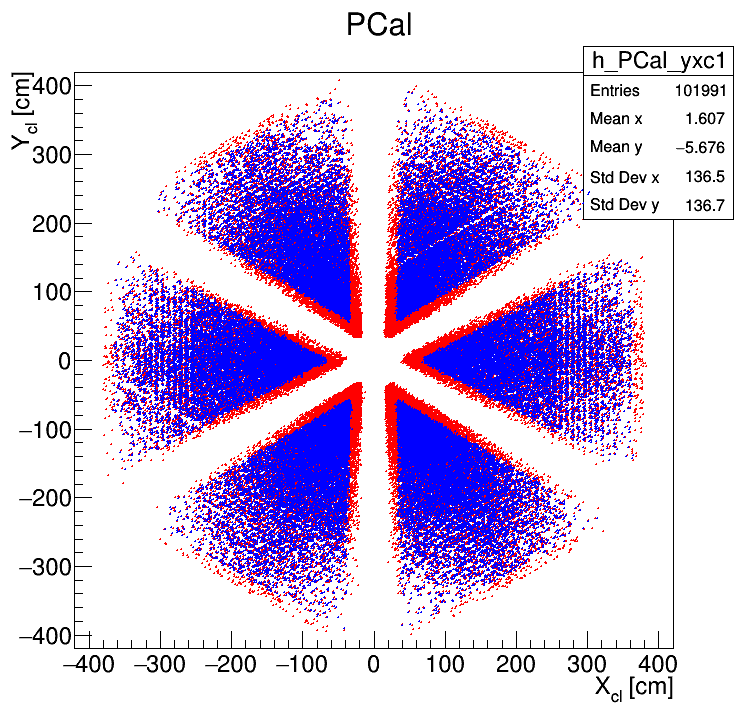
\includegraphics[width=0.24\textwidth]{img/PCal_Fiducials_4878.png}}
	\subfloat[]{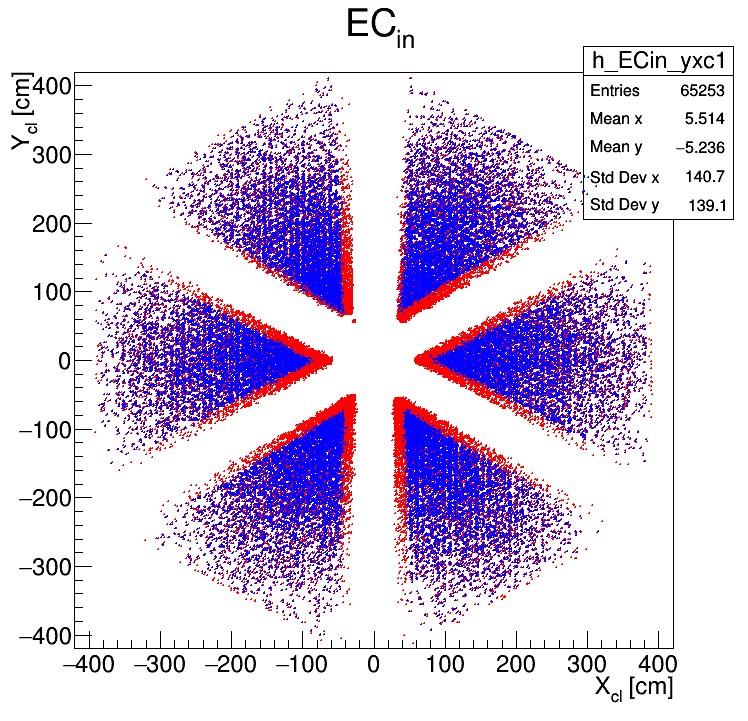
\includegraphics[width=0.24\textwidth]{img/ECin_Fiducials_4878.png}}
	\caption{Distribution of cluster coordinates of PCAL (left) and EC{in} (right).
		The scatterplots in red show all events, while the blue scatterplots show events where a cluster
		is in the fiducial region of the calorimeter (about 15 cm away from the edges).}
	\label{fig:pcal_clusters}
\end{figure}

The technique of the trigger validation is as follows. The trigger logic is configured exactly as it will be set in
an experiment, but it runs in ``tagging mode'', reporting trigger decisions into the data stream for every
randomly generated event. After several hours of running we collect at least 100 million events.

After the data is processed and the events are reconstructed, we select a subset of events with the correct
trigger time. This is done using FADC spectra for the detectors participating in the trigger logic. We need to
select events with FADC pulse times similar to those in the data obtained using the regular trigger.
Figure~\ref{fig:htcc_fadc} (a) shows typical FADC pulse arrival timing for the regular (not random) trigger.
Reconstructing and analyzing the data obtained using a random trigger, we select events with a signal in the middle
of the FADC window to make sure we do not have boundary effects when the signal region is selected. Based on the
typical pulse shape, we ignore areas with hit times below 50~ns and above 150~ns (see Fig. ~\ref{fig:htcc_fadc} (b)).

\begin{figure}[!htb]
	\centering
	\subfloat[]{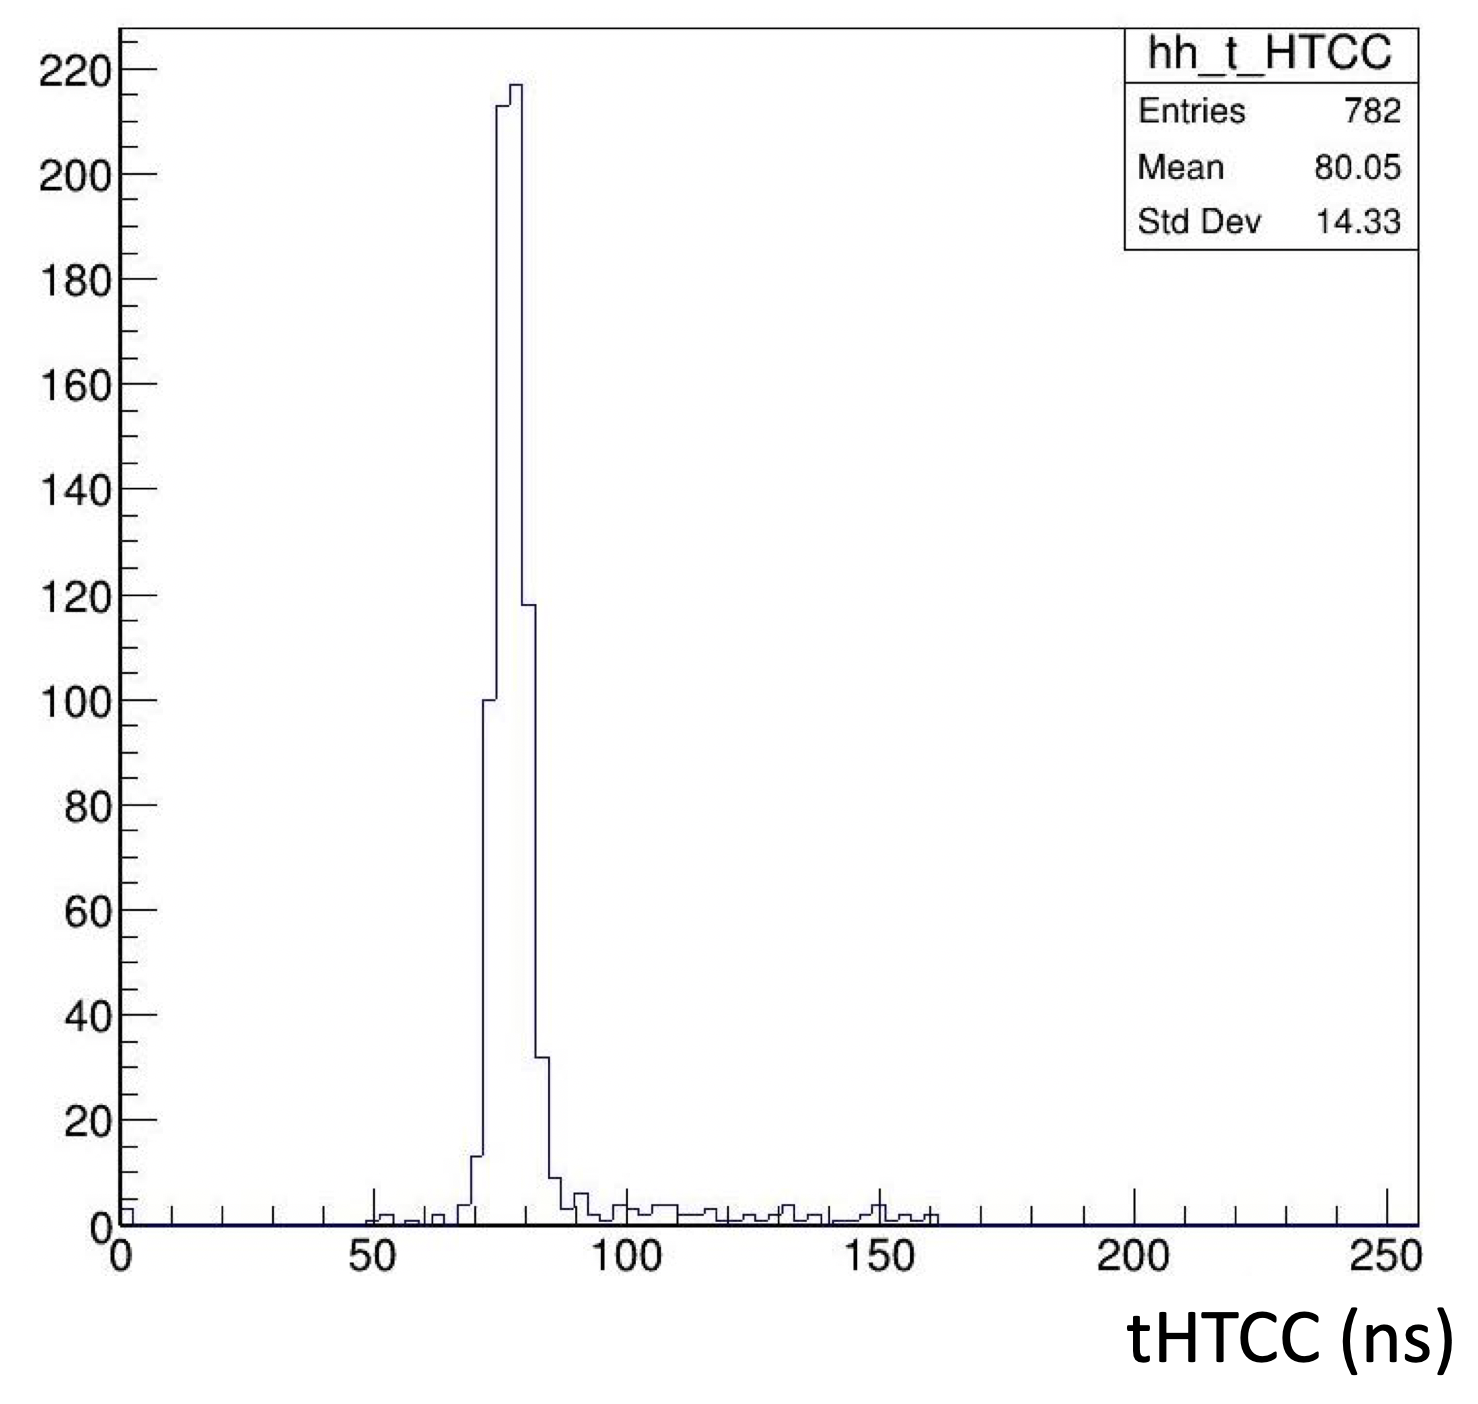
\includegraphics[width=0.24\textwidth]{img/htcc_fadc1.png}}
	\subfloat[]{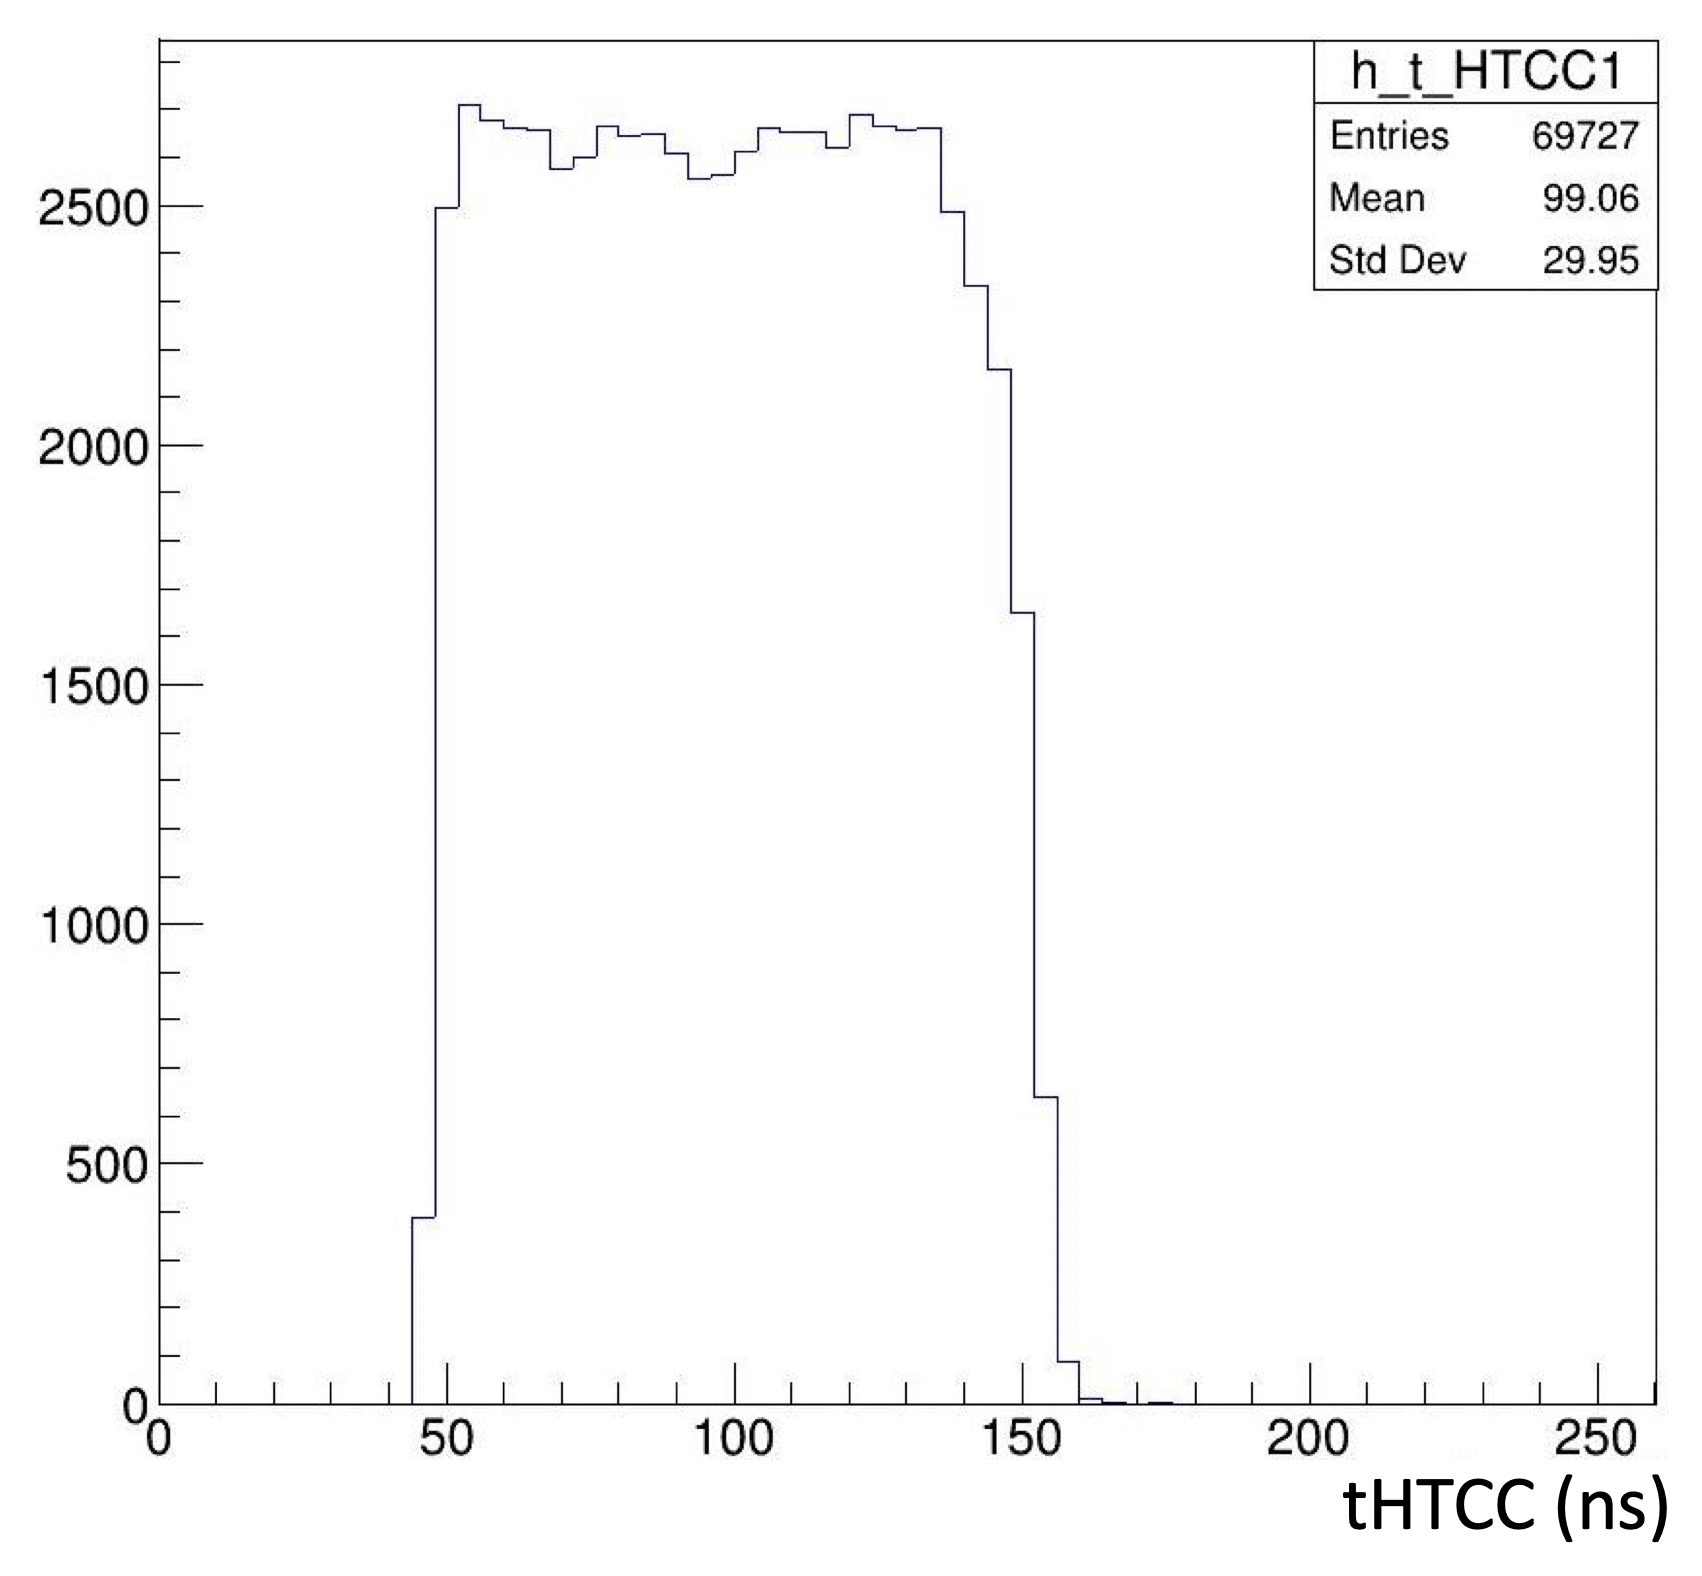
\includegraphics[width=0.24\textwidth]{img/htcc_fadc2.png}}
	\caption{HTCC FADC pulse arrival times: a) - physics triggers, b) - random trigger. Plot a) was used to select ``good''
          events from the Random Trigger runs. For such events, the FADC timing has to be at least 50 ns
          from both timing window edges to avoid boundary effects.}
	\label{fig:htcc_fadc}
\end{figure}

We typically find several thousand events that accidently fall into the correct trigger window. These events
can be used to obtain the trigger efficiency and purity assuming that our offline reconstruction software
works correctly. It should be mentioned that correct working of the offline reconstruction is an important
pre-requisite for complete trigger validation.

\subsection{Validation of the Electron Trigger}
\label{elctron_trigger_validation}
As a reminder the electron trigger logic uses responces from PCAL, EC, HTCC and DC (see eq. \ref{eq:em_trg_formula}), and as it was described in section \ref{sec:validation_random}, for trigger validation we have used a Random Trigger data. 
The $\mathrm{1^{st}}$ step in the validation of electron trigger is a selection of  events with ``clean electron''. The CLAS12 offline reconstruction software assignes PID to each reconstruction particle ({\color{Red} reference to offline recon.}) ( for electron PID=11) however in this studies we imposed additional cuts. 
In particular 
\begin{itemize}
 \item DC roads are optimized for tracks originating from the target, that is why in the offline analysis we have put a cut on the vertex ``Z'' coordinate to make sure the track originates from the target.
 \item Selected events where electron hits calorimeters (PCal and EC) in a fiducial region, to make sure the shower is fully reconstructed.
 \item Applied trigger condition cuts on offline cluster energies in the PCAL and EC, also on number of photoelectrons in HTCC.
\end{itemize}
After applying above mentioned cuts, for each of these electrons, we have checked whether the electron trigger bit is set for the corresponding sector. At the end the trigger efficiency is defined as the number of ``Bit  Set'' events over the number of all events with ``clean'' electron.
Both RG-A and RG-B experiments required to have a good (close to $100 \%$) trigger efficiency for electron above $\mathrm{2\;GeV}$. Since both PCAL and EC are sampling calorimeters, $\mathrm{2\;GeV}$ electrons will deposit only part (in average about $25\%$ in our case) of the the total energy. Then because of shower and light fluctuations some $\mathrm{2\;GeV}$ electrons will have less than $\mathrm{25\%}$ energy reconstructed in the calorimeters. Based on this, in the trigger we required the energy to be more than $\mathrm{300 \; MeV}$, which guarantee that more than $\mathrm{99\%}$ of $\mathrm{2\;GeV}$ electrons will deposit energy above the threshold.

\begin{figure}[!htb]
 \centering
 \subfloat[]{\label{fig:em_eff_Allcomponents}\grinp[width=0.25\tw]{img/All_components_65416544.pdf}}
 \subfloat[]{\label{fig:em_nphe_Miss}\grinp[width=0.25\tw]{img/nphe_missed1_65416544.pdf}}
 \caption{(a) Momentum distribution of ``Good electrons''. The brown distribution represents all ``Good electrons'', The blue histograms represents all events where the electron trigger bit was not set, the black histogram represent events, which doesn't have $\mathrm{EC}\times \mathrm{PCal}$ trigger bit, and the red one represent events that missed the electron trigger bit. (b) distribution of the number of photoelectrons for where the electron has more than $\mathrm{2\;GeV}$ energy and missed the HTCC trigger bit.}
 \label{fig:em_missed_events}
\end{figure}

Fig.\ref{fig:em_eff_Allcomponents} shows the momentum distributions of all ``Good'' electrons (in brown), electrons when electron trigger bit was not set  (in blue), when $\mathrm{EC}\times \mathrm{PCAL}$ bit was not set (in black), and red represents events when HTCC bit was not set. As one can see, above $\mathrm{2\; GeV}$ most of events have only HTCC bit missing.  Fig.\ref{fig:em_nphe_Miss} presents the distribution of the number of photoelectrons for events, which have no  HTCC trigger bit. As one can see about $\mathrm{90\%}$ of these events are    at the threshold region (reminder that in the trigger we used 2 photoelectron threshold).  The Trigger System has different from the offline reconstruction  precision of gains and pedestals values. ({\color{Red}probably Ben can comment what was the exact precision}) It could potentially create  such threshold related effects.

\begin{figure}[!htb]
 \centering
 \grinp[width=0.45\tw]{img/em_Efficiency_65416544.pdf}
 \caption{Trigger efficiency as a function of the electron momentum.}
 \label{fig:em_eff}
\end{figure}

The final efficiency is shown in the Fig.\ref{fig:em_eff}, where we can see that  the trigger efficiency is above $\mathrm{95\; \%}$
for electrons with momentum above $\mathrm{2\ GeV}$.


\subsection{Validation on beam during CLAS12 detector commissioning -  photoproduction trigger}

As described in section \ref{sec:photoproduction_trigger}, the CLAS12 photoproduction trigger requires the coincidence between one electron measured in the Forward Tagger detector, and two hadrons measured within the CLAS12 detector, in the forward or central part. The validation procedure aims to verify if, for a given event foreseeing one final-state electron in the FT acceptance and two or more hadrons scattered within the CLAS12 acceptance, the trigger system would recognize it properly, resulting in event readout. In order to validate the system with beam during commissioning, the following strategy was adopted. First, the $e^-$ detection by the FT was validated using Random Trigger runs. After this, the detection of single hadrons in CLAS12 was studied in special runs, were the only trigger source was the FT. Finally, the coincidence between the two systems was assessed.

\subsubsection{Validation of $e^-$ detection in FT}

A scattered electron in the Forward Tagger is identified as an electromagnetic shower in the Forward Tagger Calorimeter within a proper energy range, in time coincidence and geometrically matched to a hit in both layers of the Forward Tagger Hodoscope. The map providing the matching between the cluster seed position in the FT-Cal and the tiles position in the FT-Hodo was first derived by the nominal detector geometry, and then confirmed by Montecarlo simulations.

The identification of the scattered $e^-$ in the FT was validated through a similar procedure as the one adopted for the CLAS12 electron trigger discussed before, based on ``Random Trigger'' runs. Recorded events were processed through the standard CLAS12 reconstruction software and filtered, keeping only those with a reconstructed $e^-$ in the FT system. Since event readout was triggered by a random pulser, events with the reconstructed $e^-$ signal close to the margins of the readout window were also rejected.
For these events, the electromagnetic clusters found by the reconstruction software (``offline'' clusters) were compared to those reported by the trigger system and stored in the form of the trigger data banks.

The efficiency of the FT-Cal clustering algorithm in the trigger system was evaluated by comparing all ``offline'' clusters to those matched - in space and time - to an ``online'' one\footnote{The energy of ``offline'' clusters is properly corrected to account for electromagnetic shower leakage from the bak of the FT-Cal, while ``online'' clusters do not implement this. Therefore, for a given $e^-$ in the FT-Cal, there is a systematic difference between the two energies. This effect is properly taken into account when setting the energy range for $e^-$ detection in the trigger system, and does not affect the corresponding trigger efficiency.}. The efficiency was computed as:
\begin{equation}
\varepsilon=\frac{N_{trigger}}{N_{all}} \; ,
\end{equation}
where $N_{all}$ and $N_{trigger}$ are, respectively, the total number of ``offline'' clusters and the number of ``offline'' clusters matched to an ``online'' one.
The result is shown in Fig.~\ref{fig:FT_ClusterEfficiency}, reporting the FT trigger efficiency for electromagnetic clusters as a function of the corresponding corrected energy. Efficiency is higher than 97.5$\%$ in the full energy range of interest / 99.5$\%$ in the energy range above 1 GeV. The difference is mainly due to the fact that the clustering algorithm in the trigger system works on a 3x3 matrix of crystals, whereas this limitation doesn't hold in the offline reconstruction.
The efficiency of the FT-Cal / FT-Hodo matching algorithm was evaluated in a similar way, repeating previous calculation but considering only electromagnetic clusters associated to one hit in each FT-Hodo layer. The result is reported in Fig.~\ref{fig:FT_ClusterEfficiencyHODO}.

%%%%%%%%%%%%%%%%%%%%%%%%%%%%%%%%%%%%%%%%% F I G U R E %%%%%%%%%%%%%%%%%%%%%%%%%%%%%%%%%%%%%%%%%%
\begin{figure}[!htb]
 \centering
{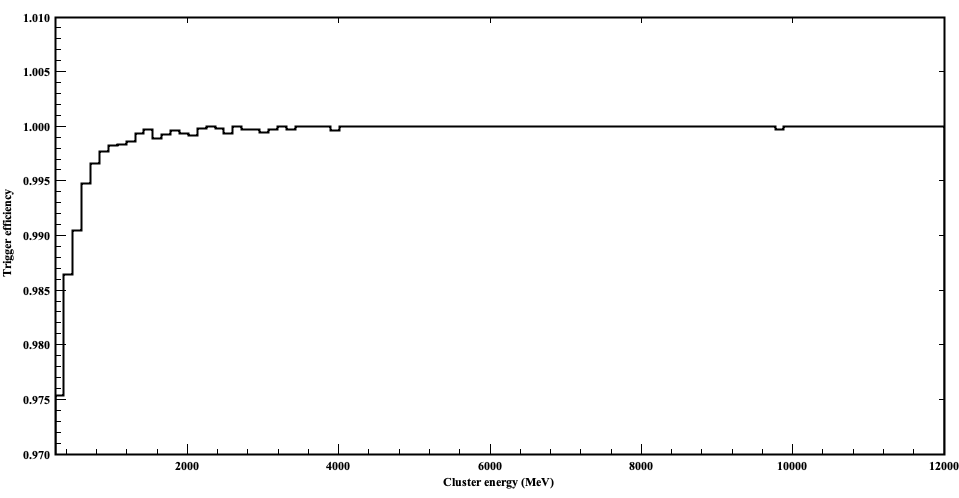
\includegraphics[width=.5\textwidth]{img/FT_ClusterEfficiency.png}}
 \caption{TODO: better figure, with errors (run 4288)}
 \label{fig:FT_ClusterEfficiency}
\end{figure}
%%%%%%%%%%%%%%%%%%%%%%%%%%%%%%%%%%%%%%%%% F I G U R E %%%%%%%%%%%%%%%%%%%%%%%%%%%%%%%%%%%%%%%%%%




\subsubsection{Validation of charged hadrons detection in CLAS12-FD}

The trigger system recognizes a charged hadron in the CLAS12 forward detector as a hit in the Forward Time-Of-Flight system (panel 1B) in time coincidence and geometrically matched to a hit in the U-bars of the Preshower Calorimeter, associated to a cluster with energy larger than a programmable threshold. The map providing the geometrical matching between FTOF counter and the PCAL U-bar was first derived by the nominal detector geometry, and then confirmed by Montecarlo simulations. To reduce the rate of random coincidences, the trigger system also requires the presence of a segment in 5 out of 6 drift chamber layers. The charged hadron identification algorithm was validated in special data-taking runs in which the Forward Tagger was the only enabled event readout source. In these runs, the trigger system was configured to report in the output trigger bank the presence of a charged hadron in any CLAS12-FD sector, as defined before. 

Recorded events were processed through standard reconstruction software and filtered, keeping only those with a well reconstructed charged track measured in CLAS12-FD. The track was required to be within the nominal acceptance of CLAS12 PCAL, and a momentum threshold of 300 MeV/c was applied. The trigger system efficiency was evaluated by comparing all reconstructed tracks to the tracks recognized by the trigger system. During commissioning, the efficiency was evaluated as a function of different observables, such as the energy deposited in the FTOF counters and in the PCAL, and the topology of the geometrical matching window. Trigger parameters were individually tuned to maximize the trigger efficiency. In the final configuration, an energy threshold of 2 MeV and 10 MeV for the FTOF counters and PCAL clusters was selected.  The result is reported in Fig.~\ref{fig:FD_TrackEfficiency}, showing the CLAS12-FD trigger efficiency for charged hadrons as a function of the track momentum. The efficiency is larger than 99$\%$ in the full momentum range, the inefficiency being dominated by threshold effects for the PCAL clusters.

%%%%%%%%%%%%%%%%%%%%%%%%%%%%%%%%%%%%%%%%% F I G U R E %%%%%%%%%%%%%%%%%%%%%%%%%%%%%%%%%%%%%%%%%%
\begin{figure}[!htb]
 \centering
{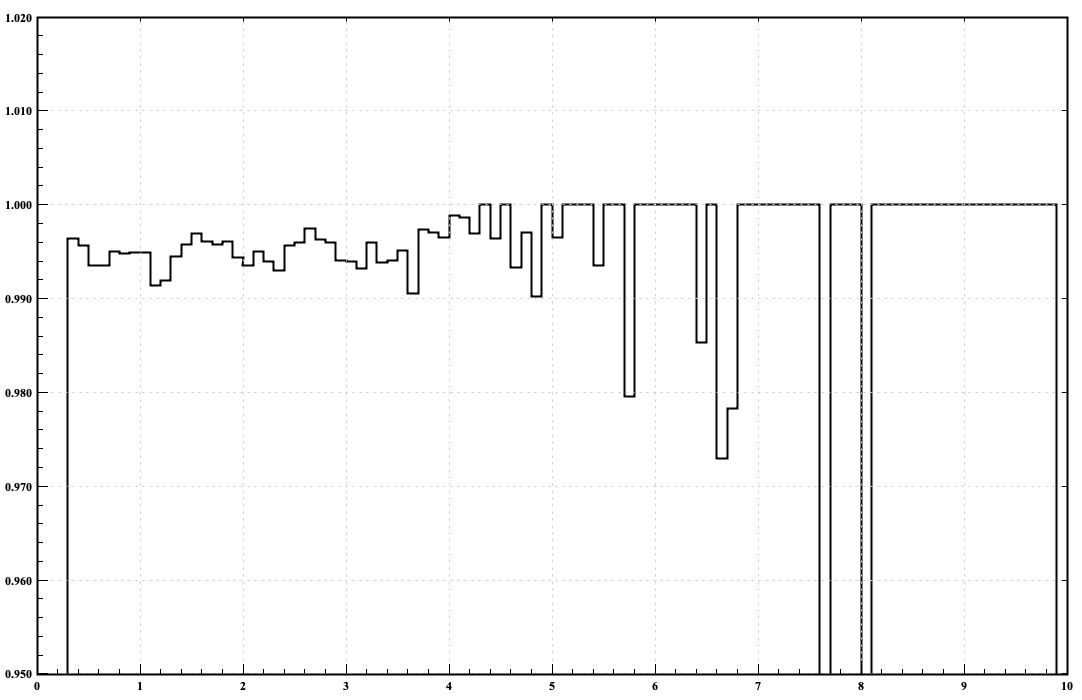
\includegraphics[width=.5\textwidth]{img/FD_TrackEfficiency.png}}
 \caption{TODO: better figure, with errors - run 5049-5050 (run4)}
 \label{fig:FD_TrackEfficiency}
\end{figure}
%%%%%%%%%%%%%%%%%%%%%%%%%%%%%%%%%%%%%%%%% F I G U R E %%%%%%%%%%%%%%%%%%%%%%%%%%%%%%%%%%%%%%%%%%



\subsubsection{Validation of charged hadron detection in CLAS12-CD}

The trigger system recognizes a charged hadron in the CLAS12 central detector as a hit in the Time-Of-Flight system (panel 1B) in time coincidence and geometrically matched to a hit in the U-bars of the Preshower Calorimeter.




\subsection{Drift Chamber-Based Trigger Components and Data-Based Dictionary}
\label{dc_dictionary}

The road dictionary for the DCs used within the Trigger System was initially generated using a fast Monte Carlo approach, where positive and negative particles in a selected momentum and angular range were randomly generated, tracked in the CLAS12 magnetic field using the CLAS ``swimmer'' developed for the offline reconstruction based on a 4th-order Runge-Kutta approach, and projected onto the DC wire planes to determine the hit position and therefore the DC wire IDs. This method has intrinsic limitation because of the approximation done in tracking the particle through the detector that does not include energy loss, multiple scattering, or other effects due to the particle interactions with the detector material.

To overcome these limitations, roads were also generated from full GEANT4 simulations of the CLAS12 detector based on the GEMC package as described in Section \ref{simulated_data_preparation}. This provides an accurate description of the relevant materials the particles travel through, resulting in a more accurate road dictionary at the expenses of a significantly higher computing time to generate the same size dictionary.

The effectiveness of these two approaches was tested by using real tracks from beam data to evaluate the completeness of the dictionaries, i.e. the fraction of tracks for which a matching road is found. This study indicated that very large statistics is needed in the dictionary-making to populate specific regions of the phase space.

As a third alternative approach, dictionaries were also produced from real tracks from beam data: in this case dictionaries with very large statistics can be produced in limited computing time with the advantage of the best accuracy in accounting both for particle interaction in matter and for the real detector geometry. These were the dictionaries that were used in the final trigger implementation.



\subsection{Final Validation Before Experiment Start-up}

Even though the Trigger System components were validated when the CLAS12 detector was commissioned, we
still have to execute our validation processes for the entire system at the beginning of every experiment. This
is necessary because different experiments request configuration changes in the Trigger System that take
advantage of its flexibility. Also, we apply firmware changes occasionally to improve the Trigger System
components based on our previous experience, and then the changes have to be validated. The final Trigger
System validation is performed by taking beam data with a random trigger (see
Section~\ref{sec:validation_random}).

The final trigger validation procedure was executed several times during the first year of CLAS12 experiments
and has proven to be very useful: bugs in the trigger firmware were found and fixed, and the trigger
configuration parameters were optimized. On one occasion a firmware bug was introduced into the PCAL Stage~1
trigger logic during the firmware update that was expected to be small and simple. The final validation procedure
revealed an irregularity in the spatial distribution of clusters (see Fig.~\ref{fig:PCAL_bug_data}) (it also shows
one CLAS12 sector is missing but this was another problem unrelated to the Trigger System). Since the PCAL
Stage~1 trigger firmware is implemented in C++/HLS, the Geant4 data sample was reprocessed through the
C++ firmware implementation (see Fig.~\ref{fig:PCAL_bug_hls}), and the problem was confirmed and
subsequently found and fixed. The firmware was recompiled and reloaded, and the final trigger validation was
repeated showing that the problem was fixed. It took only several hours between finding the problem and being
ready to run again. Every experiment in CLAS12 begins with a complete Trigger System validation. 

\begin{figure}[hbt]
	\centering
	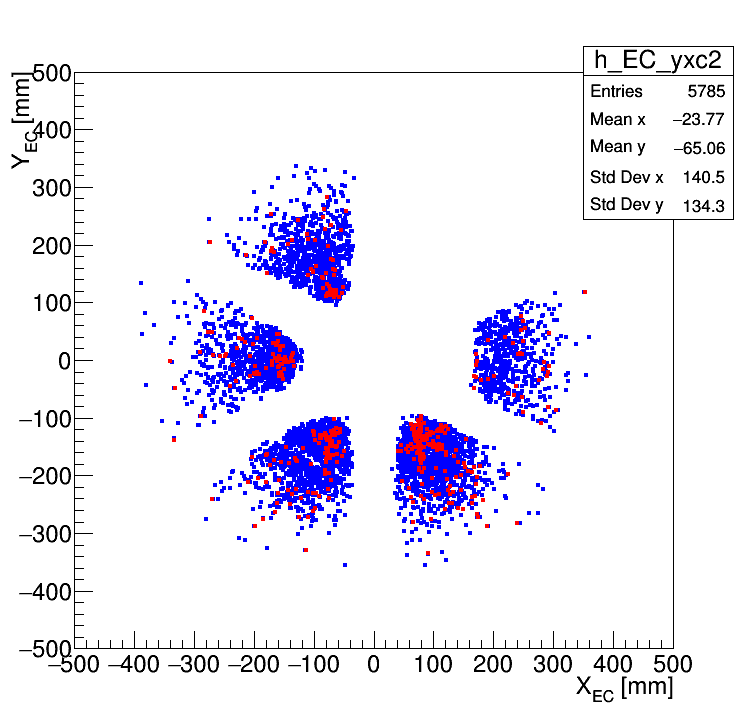
\includegraphics[width=1.0\columnwidth,keepaspectratio]{img/PCAL_bug_data.png}
	\caption{PCAL trigger bug in beam data. The red crosses inside the blue areas correspond to trigger
          inefficiencies. This was discovered during beam data processing.}
	\label{fig:PCAL_bug_data}
\end{figure}

\begin{figure}[hbt]
	\centering
	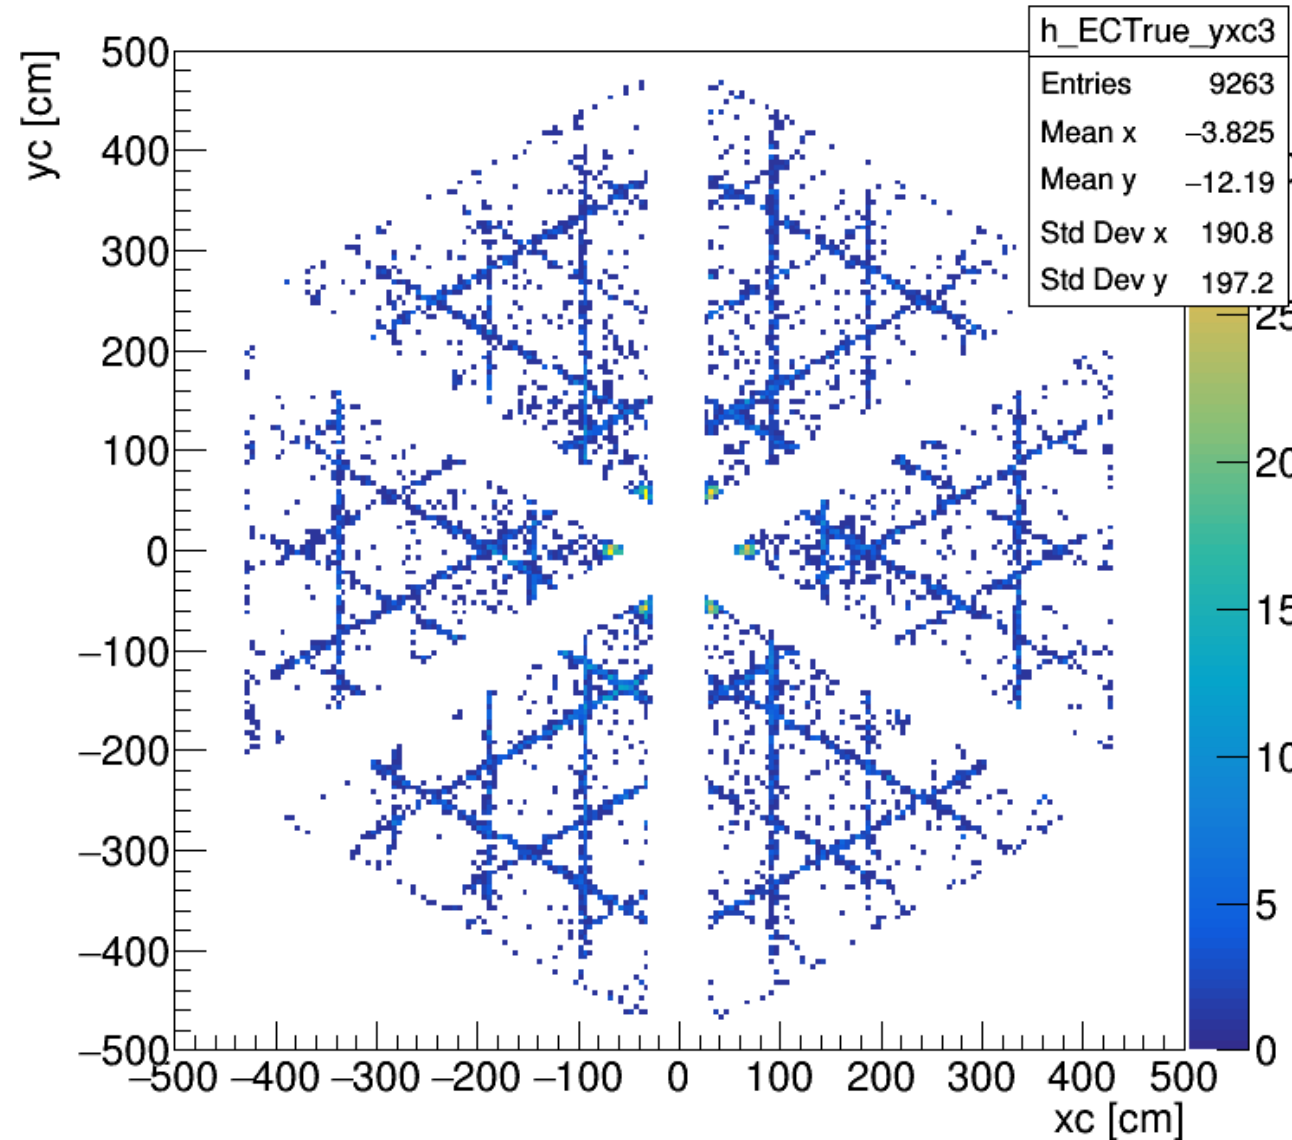
\includegraphics[width=1.0\columnwidth,keepaspectratio]{img/PCAL_bug_hls.png}
	\caption{PCAL trigger bug in Geant4 simulation. The blue lines correspond to trigger inefficiencies. This
          is visible much better in simulation than in beam data, and points to an exact problem.}
	\label{fig:PCAL_bug_hls}
\end{figure}

\section{Performance}The HTCC is one of the major CLAS12 systems used in experiments with the electron beam. The most important aspects of the HTCC performance are that it provides good timing, high electron detection efficiency, high signal strength, and high rejection factor of charged pions. All these parameters are critical for the quality of the data obtained in experiments since the detector, in combination with the forward calorimeter [ref. to ECAL], provides a fast trigger signal for CLAS12. As shown in section 6 the MC prediction for the HTCC for electrons is $\approx$100\%. Fig.~\ref{fig:RAFO_2GeV}. shows the experimentally measured electron detection efficiency for elastically scattered electrons at 2 GeV. The corresponding thresholds applied were approximately 2.5 photoelectrons. Measurements were performed using a special procedure with a random trigger that was not correlated with the HTCC. There were observed 27 events not detected by the HTCC due to the applied threshold. As shown, the electron detection efficiency is $\eta$ = (99$\pm$0.2)\%, which is in good agreement with the MC estimate. This result can be considered as a conservative estimate due to relatively high threshold used in measurements. Moreover, electrons travel a longer distance in the radiator gas (10 \% to 30 \% difference depending on a scattering angle). For these electrons the signal strength is higher, and therefore the detection efficiency is higher also as compared with the aforementioned efficiency for the elastically scattered electrons.   

\begin{figure}[!ht]
    \centering
    \includegraphics[width=1.0\linewidth,trim={0.0cm 0.0cm 0.0cm 0.0cm},clip]{images/RAFO_2GeV.jpg}
    \caption{Electron detection efficiency for elastically scattered electrons at 2 GeV. Data are obtained with the random trigger not correlated with the HTCC or other detector components of CLAS12.}
    \label{fig:RAFO_2GeV}
\end{figure}

Fig.~\ref{fig:positivePNPEC6595} shows the response of the detector in a wide range of particle momentum. The increase of number of events at high momenta is due to registration of charged pions (above threshold of their registration in the HTCC) and this is clearly illustrated.

\begin{figure}[!ht]
    \centering
    \includegraphics[width=1.0\linewidth,trim={0.0cm 0.0cm 0.0cm 0.0cm},clip]{images/positivePNPEC6595.png}
    \caption{Distributions of the HTCC response in a wide momentum range, including the region beyond the threshold of charged pion registration. Data obtained for positrons and $\pi^{+}$-mesons.}
    \label{fig:positivePNPEC6595}
\end{figure}

\begin{comment}
As shown bellow in the Fig.~\ref{fig:avgNPE_Theta_Phi_Dev_Build-2_NO_HOLES} the signal strength goes up for the utmost mirrors (large electron scattering angles). This is because electrons travel a longer distance in the radiator gas (10\% to 30\% difference depending on angle.) In other words the electron detection efficiency obtained for elastically scattered electrons at 2 GeV can be considered as as a conservative estimate for the efficiency of electron detection at larger angles.
\end{comment} 

The signal strength in the HTCC depends on the actual properties of the mirror facets, such as their final shape and reflectance. The accuracy of the combined mirror assembly and the alignment of the HTCC components (mirror, PMTs, Winston Cones), and the composition of the radiator gas all influence the final results. The FADC histogram of  the typical signal strength distribution obtained in one half-sector \#1 and \#2 of Sector 1 is shown in Fig.~\ref{fig:Signal_S1_HS1_HS2_R1_R2}. The signal strength for scattered electrons averaged over all HTCC channels is shown in Fig.~\ref{fig:Average_HTCC_Signal}. The experimentally measured mean value of 16.3 phe is close to Monte-Carlo simulation results, (see Fig.~\ref{fig:10cm_Targ_5T_Field_Phi}).

\begin{figure}[!ht]
    \centering
    \includegraphics[width=1.0\linewidth,trim={0.0cm 0.0cm 0.0cm 0.0cm},clip]{images/Signal_S1_HS1_HS2_R1_R2.jpg}
    \caption{Typical distributions of the signal strength in channels covering polar angles in the range of $5^\circ$ to $12.5^\circ$ (Ring 1) and $12.5^\circ$ to $20.0^\circ$ (Ring 2) within azimuthal interval of $60^\circ$.}
    \label{fig:Signal_S1_HS1_HS2_R1_R2}
\end{figure}

\begin{figure}[!ht]
    \centering
    \includegraphics[width=1.0\linewidth,trim={0.0cm 0.0cm 0.0cm 0.0cm},clip]{images/Average_HTCC_Signal.jpg}
    \caption{The HTCC average signal strength for electrons from beam data.}
    \label{fig:Average_HTCC_Signal}
\end{figure}

Fig.~\ref{fig:HTCC_Response_run4013} shows the HTCC response for different electron momenta. Fig.~\ref{fig:avgNPE_Theta_Phi_Dev_Build-2_NO_HOLES}  shows the distribution of the HTCC response over the entire face of the mirror in the $x-y$-plane. Similar distribution is shown in Fig.~\ref{fig:avgNPE_XY_Dev_Build_02npe} obtained at the lower electron detection threshold of 0.2 photoelectrons. At the large electron scattering angles in range of 27.5$^\circ$ to 35$^\circ$, the statistics is lower. Fig.~\ref{fig:statistics_Theta_Phi_Dev_Build_NO_HOLES} shows the distribution of statistics in all 6 sectors. The data shows that the integrated signal strength is about 16.5 photoelectrons.

\begin{figure}[!ht]
    \centering
    \includegraphics[width=1.0\linewidth,trim={0.0cm 0.0cm 0.0cm 1.73cm},clip]{images/HTCC_Response_run4013.png}
    \caption{The HTCC response for electrons: signal strength vs. momentum at 10.6 GeV energy.}
    \label{fig:HTCC_Response_run4013}
\end{figure}

\begin{figure}[!ht]
    \centering
    \includegraphics[width=1.0\linewidth,trim={0.0cm 0.0cm 0.0cm 1.67cm},clip]{images/avgNPE_Theta_Phi_Dev_Build-2_NO_HOLES.png}
    \caption{The HTCC response (in $N_{phe}$) for electrons in $x-y$-plane of the mirror.}
    \label{fig:avgNPE_Theta_Phi_Dev_Build-2_NO_HOLES}
\end{figure}

\begin{figure}[!ht]
    \centering
    \includegraphics[width=1.0\linewidth,trim={0.0cm 0.0cm 0.0cm 1.67cm},clip]{images/avgNPE_XY_Dev_Build_02npe.png}
    \caption{The HTCC response (in $N_{phe}$) for electrons in $x-y$-plane of the mirror at the electron detection threshold of 0.2 photoelectrons.}
    \label{fig:avgNPE_XY_Dev_Build_02npe}
\end{figure}

\begin{figure}[!ht]
    \centering
    \includegraphics[width=1.0\linewidth,trim={0.0cm 0.0cm 0.0cm 1.67cm},clip]{images/statistics_Theta_Phi_Dev_Build_NO_HOLES.png}
    \caption{Distribution of statistics in all 6 sectors.}
    \label{fig:statistics_Theta_Phi_Dev_Build_NO_HOLES}
\end{figure}

We also note that in cases when the electrons cross the mirror close to its edges (at approximately at 5$^\circ$ and 35$^\circ$) one should expect unavoidable losses in the signal strength: some part of the Cherenkov light just passes by the mirror. As far as the internal borders between adjacent mirrors are concerned, there are similar losses that take place and are finally partially compensated due to the complete azimuthal symmetry of the detector, see Fig.~\ref{fig:avgNPE_Theta_Phi_Dev_Build-2_NO_HOLES}. The width of that area along internal boundaries that is deformed in the direction normal to the mirror face due to the shrinkage of the glue is estimated between $\sim$5 to $\sim$10 mm. This area includes the technological zone ~0.5 mm of width that is not reflecting the light at all. As a result these regions (width up to $\sim$10 mm) along internal boundaries between mirror facets defuse the light impinging the area, and therefore the signal strength is reduced. this edge effect is normal for the given design of the detector.


\section{Acknowledgements}

We appreciate the contribution of J.  Andresen, C. Britton, S. Chappa, A. Dyer, J. Hoff, V. Re, and T. Zimmerman to the design of the HFCB. We are grateful to administrative, engineering, and technical staff of Fermilab Silicon Detector Facility for excellent work on module assembly.

\section{Conclusions}

The SVT is installed in the CLAS experimental hall, performance of modules measured during detector integration has been confirmed. No channels were lost during the installation. SVT barrel has been electrically  tested with number of defective channels 0.1$\%$, well within the specification. The chip average ENC noise is uniform $\sim$1600 e in normal operating conditions. There is no evidence of coherent noise between the modules and other components. The tracker has been commissioned with cosmic rays and integrated as part of  CLAS central detector. Tracking performance was confirmed with beam data and matches physics requirements. 




\section{References}

%%\bibliography{bibfile}
%%\bibliographystyle{elsarticle-num}


\begin{thebibliography}{99}

\bibitem{daq-ref}
S.~Boyarinov {\it et al.}, {\it ``The CLAS12 Data Acquisition System''}, see this issue.

\bibitem{overview-ref}
V.D.~Burkert {\it et al.}, {\it ``The CLAS12 Spectrometer at Jefferson Laboratory''}, see this issue.

\bibitem{clas-nim}
B.A.~Mecking {\it et al.}, Nucl. Inst. and Meth. {\bf A503}, 513 (2003).

\bibitem{cnd-ref}
J. Bettane {\it et al.}, {\it ``The CLAS12 Central Neutron Detector''}, see this issue.

\bibitem{ftof-ref}
D.S. Carman {\it et al.}, {\it ``The Forward Time-of-Flight System for CLAS12''}, see this issue.

\bibitem{ctof-ref}
D.S. Carman {\it et al.}, {\it ``The Central Time-of-Flight System for CLAS12''}, see this issue.

\bibitem{htcc-ref}
Y. Sharabian {\it et al.}, {\it ``The CLAS12 High Threshold Cherenkov Counter''}, see this issue.

\bibitem{ec-ref}
G. Asryan {\it et al.}, {\it ``The CLAS12 Forward Electromagnetic Calorimeter''}, see this issue.

\bibitem{dc-ref}
M. Mestayer {\it et al.}, {\it ``The CLAS12 Drift Chamber System''}, see this issue.

\bibitem{ft-ref}
NNN {\it et al.}, {\it ``The CLAS12 Forward Tagger System''}, see this issue.

\bibitem{hls-ref}
HLS {\it et al.}, {\it ``VIVAO High Level Synthesis''}, yyy.

\end{thebibliography}


\end{document}








